\documentclass[11pt]{article}
%edet|003|=)
\title{\textbf{\em edet \em White Paper}\linebreak\small{Version 0.2.1}}
\author{Yann Gohh}
\date{April 2026}
\usepackage{graphicx}
\usepackage[T1]{fontenc}
\usepackage{amsmath}
\usepackage{amssymb}
\usepackage{tikz}
\usepackage{pgf-umlsd}
\usepackage{array}
\usepackage{hyperref}
\emergencystretch=3em
\hypersetup{
    colorlinks=false,
    pdfborder={0 0 0},
    hidelinks
}

\newtheorem{theorem}{Theorem}[section]
\newtheorem{lemma}[theorem]{Lemma}
\newtheorem{definition}[theorem]{Definition}
\newtheorem{corollary}[theorem]{Corollary}
\newtheorem{remark}[theorem]{Remark}
\newtheorem{property}{Property}[section]
\newenvironment{note}{\noindent\textbf{Note.}}{\par\medskip}

% Manual proof and qed definitions (replaces amsthm)
\newcommand{\qed}{\hfill}
\newenvironment{proof}{\noindent\textbf{Proof.}}{\qed$\square$\par\medskip}

% Redefine \mess to avoid creating nodes with special chars in names
\renewcommand{\mess}[4][0]{
  \stepcounter{seqlevel}
  \path
  (#2)+(0,-\theseqlevel*\unitfactor-0.7*\unitfactor) node (mess from) {};
  \addtocounter{seqlevel}{#1}
  \path
  (#4)+(0,-\theseqlevel*\unitfactor-0.7*\unitfactor) node (mess to) {};
  \draw[->,>=angle 60] (mess from) -- (mess to) node[midway, above]
  {#3};
}

\begin{document}

\maketitle


\newpage
\begin{abstract}
Human society's economy is described meaningfully in terms of propagation of debt, opposed to propagation of credit which is the current mode. This paper proposes a novel approach to value transfer in modern societies where electronic currency becomes standard, introducing a fundamental difference with respect to cryptocurrencies: the absence of profit.

A key challenge in any decentralized debt-propagation system~\cite{fugger2004,lietaer2001,greco2009} is distinguishing virtuous peers from malicious ones without a central authority. Modern decentralization technologies allow for impartial, distributed control, making the vision of accounting for transferred debt instead of transferred credit possible.

This paper proposes the \em edet \em protocol, a mathematically grounded reputation framework based on the EigenTrust algorithm~\cite{kamvar2003}. Trust is derived from a single observable: \emph{whether a debtor satisfies their obligations}. The protocol incorporates a multi-layered defense against a comprehensive set of adversarial strategies: (1)~\textbf{Sybil ring attacks}, where colluding identities inflate apparent trustworthiness; (2)~\textbf{gateway attacks}, where a trusted node routes trust to a malicious cluster; (3)~\textbf{slacker attacks}, where nodes free-ride without contributing; (4)~\textbf{whitewashing}, where a node abandons a defaulting identity to escape reputation damage; (5)~\textbf{circular trading}, where colluding nodes manufacture fake satisfaction evidence; (6)~\textbf{intermittent (strategic oscillation) attacks}, where an attacker alternates between honest and dishonest epochs to stay below detection thresholds; (7)~\textbf{build-then-betray attacks}, where a node accumulates trust over many epochs before defecting; (8)~\textbf{economic griefing}, where a node strategically triggers failures to damage a target's reputation; (9)~\textbf{newcomer exploitation}, where fresh identities are used to probe the network at minimal cost; (10)~\textbf{transaction spam}, where high-frequency low-value activity attempts to saturate trust channels; (11)~\textbf{coordinated market manipulation}, where a colluding cluster targets specific nodes with mass defaults; (12)~\textbf{double-contracting}, where a debtor takes on more debt than their capacity allows via concurrent contracts; and (13)~\textbf{eclipse and routing attacks}, where a node's local DHT view is corrupted to distort its subjective trust computation.

For each attack, we provide formal bounds on extractable value or provably zero expected gain. The protocol includes a confidence-weighted local trust model, a logarithmic volume-maturation tolerance ramp, a rolling recent-failure-rate window for behavioral-switch detection, a witness-based failure contagion mechanism, and a trust banking cap to prevent accumulate-then-defect strategies. We provide formal convergence proofs, isolation theorems, and economic break-even analyses.
\end{abstract}
\pagebreak

\tableofcontents

\pagebreak

\begin{flushright}
\hfill \break
\hfill \break
\hfill \break
\hfill \break
\hfill \break
\hfill \break
\hfill \break
\hfill \break
\em ''The great polyp had become the Master's last disciple for a very simple reason. It was immortal. The billions of individual cells from which its body was built would die, but before that happened they would have reproduced themselves. At long intervals the monster would disintegrate into its myriad separate cells, which would go their own way and multiply by fusion if their environment was suitable. During this phase the polyp did not exist as a self-conscious, intelligent entity - and here Alvin was irresistibly reminded of the manner in which the inhabitants of Diaspar spent their quiescent millenniums in the city's memory Banks.''\em

Arthur C. Clarke: The City and the Stars

\end{flushright}

\pagebreak

\section{Introduction}

\em edet \em is a distributed ledger for economic transactions. It opposes all existing cryptocurrencies at the time of writing because it transfers the value of debt, instead of the value of credit.

Debt is contracted by the buyer in exchange for a good or service from the seller, and such exchange is called a \emph{transaction}. The seller may direct the system to drain accumulated debt from third-party wallets, creating a cascading debt-propagation mechanism akin to donation or crowdfunding.

The fundamental challenge in a debt-based system is preventing abuse: without countermeasures, a peer could accumulate debt and abandon their wallet, or a cluster of colluding peers could artificially inflate their apparent trustworthiness. Unlike credit-based systems where the token itself carries value, in a debt system the \emph{reputation} of the debtor is the critical asset.

This paper presents a solution grounded in spectral graph theory and the theory of Markov chains. The core insight is that trust should not be an ad-hoc indicator maintained alongside debt, but rather the stationary distribution of a random walk on the transaction graph, where edge weights are determined by observable economic behavior (debt satisfaction vs.\ default).

\subsection{Why Debt, Not Credit?}
\label{sec:debt_vs_credit}

A natural question is whether transferring debt rather than credit has any formal economic advantage, or whether a seller could simply reprice goods to extract the same speculative rent through debt capacity accumulation. We address this with a minimal two-agent model.

\paragraph{Credit-based baseline.}
In a credit system, each agent holds a balance $B_i \geq 0$ of transferable tokens. A transaction from buyer $b$ to seller $s$ of value $\delta$ moves $\delta$ tokens from $b$ to $s$: $B_b \leftarrow B_b - \delta$, $B_s \leftarrow B_s + \delta$. Tokens are \emph{scarce}: the total supply $\sum_i B_i$ is fixed. Holding tokens is rational if their future value is expected to rise; this creates a speculative demand $\sigma \geq 0$ for tokens as a store of value, independent of transaction demand. In equilibrium, an agent with tokens worth $B_s$ in transaction utility may demand a premium of $\sigma \cdot B_s$ to part with them, effectively raising prices by the speculative factor $1 + \sigma / \bar{v}$ where $\bar{v}$ is the average transaction value.

\paragraph{Debt-based alternative.}
In a debt system, no scarce token exists. A transaction from $b$ to $s$ of value $\delta$ creates a debt contract: $b$ owes $\delta$ to $s$. However, \emph{holding debt is costly}: the debtor's credit capacity $\text{Cap}_b$ is reduced by the outstanding debt (capacity check: $\text{Debt}(b) + \delta \leq \text{Cap}_b$), and failure to transfer debt before maturity reduces reputation. There is no incentive to accumulate debt as a store of value: more debt means less capacity, not more. Conversely, creditors benefit from being repaid (satisfaction increments $S_{ij}$, building reputation) and have no motive to hoard debt obligations.

\paragraph{Formal comparison.}
Let utility of agent $i$ in period $T$ be $U_i = \sum_{t=1}^T v_{it} - c_{it}$, where $v_{it}$ is value received from transactions and $c_{it}$ is cost incurred. In the credit model:
\begin{equation}
    c^{\text{credit}}_{it} = \delta_{it} \cdot (1 + \sigma_t)
\end{equation}
where $\sigma_t \geq 0$ is the speculative premium at time $t$. In the debt model:
\begin{equation}
    c^{\text{debt}}_{it} = \delta_{it} + \rho \cdot \max(0,\, \text{Debt}(i) - \text{Cap}_i)
\end{equation}
where $\rho > 0$ is the penalty for over-leveraging (reputation loss, contract failure). Since $\sigma_t \geq 0$ by definition and $\rho \cdot \max(0, \cdot) = 0$ for a solvent agent, we have:

\begin{property}[Absence of Speculative Premium]
In the edet debt model, a solvent agent ($\text{Debt}(i) \leq \text{Cap}_i$) pays $c^{\text{debt}}_{it} = \delta_{it}$: the exact transactional value with no speculative markup. In any credit model with positive speculative demand $\sigma_t > 0$, the effective transaction cost is strictly higher: $c^{\text{credit}}_{it} > \delta_{it}$.
\end{property}

\begin{remark}[Scope of the Claim]
This property eliminates speculative rent on the \emph{medium of exchange itself}. It does not prevent sellers from pricing goods above marginal cost for other reasons (market power, quality signaling, etc.). The edet protocol removes one specific source of systemic over-pricing — the scarcity premium on the transactional medium — without imposing price controls at the goods layer.
\end{remark}

\begin{remark}[Credit Capacity as Bounded Privilege]
One might object that credit capacity $\text{Cap}_i$ plays the role of a scarce token: high-reputation agents have more capacity and thus transactional advantage. The key difference is that capacity is \emph{earned through observable behavior} (debt satisfaction) and \emph{consumed by use} (outstanding debt reduces available capacity). It cannot be hoarded passively: an agent who accumulates capacity without transacting sees their relative capacity shrink as the acquaintance graph expands. There is no ``sitting on capacity'' strategy analogous to holding tokens off-market.
\end{remark}

\subsection{Contributions and Structure}
The contributions of this paper are:
\begin{enumerate}
    \item A \textbf{formal reputation model} (Section~\ref{sec:reputation}) combining bilateral satisfaction/failure counters, confidence-weighted local trust, logarithmic volume-maturation tolerance, and a rolling recent-failure-rate window for behavioral-switch detection, all with provable convergence (Theorem~\ref{thm:convergence}) and Sybil resistance (Theorem~\ref{thm:sybil}).
    \item A \textbf{credit capacity function} (Section~\ref{sec:capacity}) that maps subjective EigenTrust scores to economic privilege, with a trust banking cap bounding the leverage any single bilateral relationship can contribute, and scale-invariant Dunbar-bounded acquaintance sets.
    \item A \textbf{three-path transaction lifecycle} (Section~\ref{sec:capacity}) distinguishing trial (PATH~0), first-contact claim-based (PATH~1), and repeat bilateral (PATH~2) transactions, with a debt velocity factor penalizing buy-without-sell accumulation patterns.
    \item A \textbf{support escrow mechanism} (Section~\ref{sec:capacity}) enabling cascading debt acceleration via co-signed contracts, with proportional co-signer contagion on default and a formal disadvantage function bounding creditor risk.
    \item A \textbf{bootstrapping mechanism} (Section~\ref{sec:bootstrap}) for new entrants via sponsored vouching with asymmetric slashing ($X \times \delta$ against sponsors), capacity liquidation on sponsor insolvency, and trial transaction velocity limits --- allowing participation without conflation with malicious actors.
    \item \textbf{Formal security analysis} (Section~\ref{sec:security}) covering thirteen attack categories: Sybil rings, gateway, slacker, whitewashing, circular trading, intermittent oscillation, build-then-betray, economic griefing, newcomer exploitation, transaction spam, coordinated market manipulation, double-contracting, and eclipse/routing attacks --- each with a formal bound or isolation proof.
    \item A \textbf{formal properties summary} (Section~\ref{sec:security}) collecting all security guarantees as a single reference table of theorems, corollaries, and bounds.
    \item An \textbf{implementation} on Holochain (Section~\ref{sec:implementation}) where reputation is computed \emph{subjectively} per-node via a bounded BFS subgraph, with epoch-scoped caching, ReputationClaim-based first-contact fallback, and a full parameter governance table (Appendix~\ref{sec:parameters}).
\end{enumerate}

\section{System Model}
\label{sec:model}

\subsection{Notation and Parameters}

The following symbols and parameters are used throughout this paper. For a detailed analysis of parameter sensitivity and rationale, see Appendix~\ref{sec:parameters}.

\begin{center}
\begin{tabular}{|l|l|p{7cm}|}
\hline
\textbf{Symbol} & \textbf{Value} & \textbf{Meaning} \\
\hline
\hline
\multicolumn{3}{|c|}{\textbf{Graph and Transactions}} \\
\hline
$\mathcal{G} = (V, E)$ & --- & Network graph of agents (vertices) and transactions (edges) \\
$\delta$ & --- & Transaction value (debt principal) \\
$D_i$ & --- & Total outstanding debt of node $i$ \\
$\text{Cap}_i$ & --- & Maximum credit capacity of node $i$ \\
$V_{\text{staked}}$ & --- & Capacity staked by a node's vouchers (0 for unvouched identities) \\
$S_{ij}$, $F_{ij}$ & --- & Bilateral satisfaction and failure counters between $i$ and $j$ \\
\hline
\multicolumn{3}{|c|}{\textbf{EigenTrust Reputation}} \\
\hline
$\alpha$ & $0.08$ & Mixing factor (weight of personalized pre-trust vector $\mathbf{p}_i$) \\
$\epsilon$ & $0.001$ & Convergence threshold for power iteration \\
$t_i^{(obs)}$ & --- & Subjective reputation of node $i$ as computed by observer \\
$t_{\text{baseline}}$ & $\alpha / |\mathcal{A}|$ & Noise floor; trust of an unknown but vouched node \\
\hline
\multicolumn{3}{|c|}{\textbf{Protocol Constraints}} \\
\hline
$V_{\text{base}}$ & $1000$ & Denomination constant for trial thresholds and capacity bounds \\
$\beta$ & $5000$ & Capacity scaling constant (logarithmic reputation multiplier) \\
$\eta$ & $0.05$ & Trial fraction; a transaction is a trial iff $\delta < \eta \cdot V_{\text{base}}$ \\
$n_0$ & $50$ & Acquaintance saturation constant for the capacity ramp \\
$N_{\text{mat}}$ & $1000$ & Volume maturation threshold for full bilateral trust \\
$\tau$ & $0.12$ & Hard failure-rate tolerance (exclusion threshold) \\
$\tau_0$ & $0.05$ & Newcomer tolerance (applied to zero-history bilateral relationships) \\
$\gamma$ & $4.0$ & Penalty sharpness (controls isolation ramp) \\
$X$ & $3.0$ & Sponsor slash multiplier (asymmetric penalty) \\
$K_w$ & $10$ ep. & Recent failure window size for behavioral switch detection \\
$|\mathcal{A}|_{\max}$ & $150$ & Acquaintance set cap (eviction threshold) \\
$L_{\text{trial}}$ & $5$/ep. & Trial transaction velocity limit \\
$\Delta_{\text{drift}}$ & $300$\,s & Allowed clock skew for epoch assignment \\
\hline
\end{tabular}
\end{center}

\subsection{Network and Transactions}

The network is modeled as a directed weighted graph $\mathcal{G} = (V, E, w)$ where:
\begin{itemize}
    \item $V = \{1, 2, \ldots, N\}$ is the set of peers (wallets).
    \item $E \subseteq V \times V$ is the set of directed edges, where $(i, j) \in E$ if peer $i$ has transacted with peer $j$.
    \item $w: E \to \mathbb{R}_{\geq 0}$ assigns weights based on transaction history.
\end{itemize}

Time is discrete, indexed by \emph{epochs} $t \in \mathbb{N}$. In each epoch, a set of transactions may occur. A transaction $\text{tx}(b, s, \delta)$ transfers debt $\delta > 0$ from seller $s$ to buyer $b$: the buyer receives a good or service and contracts debt $\delta$ owed to $s$; the seller's existing debt is reduced by (at most) $\delta$ through \emph{debt transfer}.

\begin{definition}[Debt Contract]
A debt contract is a tuple $(\delta, M, t_0, c)$ where $\delta$ is the principal, $M$ is the maturity (in epochs), $t_0$ is the epoch of origination, and $c$ is the creditor (the seller who originated the debt). The contract requires the debtor to transfer the debt to new buyers by selling goods/services before maturity expires.
\end{definition}

\begin{definition}[Debt Transfer]
When a debtor $b$ with debt owed to creditor $c$ sells goods/services of value $r$ to a new buyer $b'$, the debt \emph{transfers}: buyer $b'$ now owes $\min(r, \text{Debt}(b))$ to $b$ as the new creditor. At the moment of transfer, $S_{c,b}$ increments by the transferred amount, recording $b$'s successful fulfillment of their obligation to $c$.
\end{definition}

\begin{definition}[Genesis Transaction]
A transaction where the seller has no existing debt to transfer creates \emph{genesis debt}: new debt that originates from nothing. This allows economic activity to bootstrap and prevents deadlock when all participants have zero debt.
\end{definition}

\begin{remark}[Genesis Debt Steady-State Dynamics]\label{rem:genesis_steady_state}
Genesis debt acts as the system's monetary creation mechanism: it injects new debt units when the existing debt pool is insufficient to clear a transaction. Three forces bound its growth in steady state:
\begin{enumerate}
    \item \textbf{Capacity ceiling.} Total outstanding debt is bounded above by $\sum_i \text{Cap}_i$, which grows logarithmically with reputation (not linearly with network size). Since each agent's capacity is $V_{\text{staked}} + \beta \ln(\max(1, t_i / t_{\text{baseline}})) \cdot (1 - e^{-|\mathcal{A}_i|/n_0})$ and trust scores sum to $1$, the aggregate capacity grows at most logarithmically in network size.
    \item \textbf{Expiration destruction.} Contracts that reach maturity without full transfer are expired, destroying the remaining principal and recording a failure~$F$. In a network with average failure rate $\bar{r}$, approximately $\bar{r}$ of outstanding debt is destroyed per maturity cycle ($M_{\min}$ epochs).
    \item \textbf{Cascade absorption.} The support cascade (Section~\ref{sec:protocol}) drains existing debt from beneficiaries before resorting to genesis creation, reducing the genesis fraction as the network's circulating debt pool grows. Well-connected networks with active support breakdowns produce minimal genesis debt in steady state.
\end{enumerate}
In the transient phase (early epochs), the genesis ratio (genesis debt per unit of transaction volume) is high ($\approx 1$) because no debt exists to transfer. As the debt pool builds through the first $1$--$2$ maturity cycles, the genesis ratio decays to a stable floor determined by the network's support connectivity and trade balance. Empirical simulation (Metric~12, Section~\ref{sec:verification}) confirms that the genesis ratio converges, and that the utilization ratio $\sum_i D_i / \sum_i \text{Cap}_i$ remains bounded well below $1$.
\end{remark}

\begin{definition}[Vouch Transaction]
A special transaction $\text{vouch}(s, n, \lambda)$ where a sponsor $s$ locks amount $\lambda$ of their own valid capacity to bootstrap a new entrant $n$. The entrant gains $V_{\text{staked}} = \lambda$ as their initial capacity. If $n$ defaults on an amount $\delta$, the sponsor $s$ is asymmetrically slashed by $X \cdot \delta$ (where $X > 1$ is the \emph{slash multiplier}) from their staking balance. Furthermore, the default $\delta$ is directly counted as a failure $F$ for the sponsor $s$ by the creditor (Reputational Contagion). This mechanism replaces ``free entry'' with a staked and socially accountable entry, ensuring Sybil resistance.

\emph{Capacity liquidation}: if the sponsor's staking balance falls below the locked amount $\lambda$ due to accumulated slashing, the vouchee's capacity is proportionally reduced: $\text{Cap}_n \leftarrow \lambda' = \text{staking\_balance}(s)$. If the balance reaches zero, the vouch is dissolved and $\text{Cap}_n$ reverts to $0$. This prevents a slashed sponsor from continuing to backstop new entrants beyond their remaining stake.
\end{definition}

\begin{theorem}[Vouching-Ring Attack Bound]\label{thm:vouch_ring}
Let $\mathcal{R} = \{v_1, \ldots, v_k\}$ be a ring of $k$ Sybil identities with total staked capacity $\Lambda = \sum_{i} \lambda_i$, where each $v_i$ vouches for $v_{i+1 \bmod k}$. Suppose the ring attempts a coordinated exit: all vouchees simultaneously default on their maximum vouched capacity. Then the total value extracted before all vouches are dissolved is bounded by:
\begin{equation}
    E_{\text{ring}} \leq \frac{\Lambda}{X}
\end{equation}
where $X > 1$ is the slash multiplier. For $X = 3$, $E_{\text{ring}} \leq \Lambda / 3$.
\end{theorem}

\begin{proof}
Consider a single vouch $\text{vouch}(s, n, \lambda)$ with $s, n \in \mathcal{R}$. If $n$ defaults on $\delta$, the sponsor $s$ is slashed by $X \cdot \delta$. The ring can extract at most $\lambda$ before $s$'s staking balance is exhausted at $X \cdot \delta = \lambda$, i.e., $\delta_{\max} = \lambda / X$.

Summing over all $k$ vouches in the ring (each with staked capacity $\lambda_i$):
\[
    E_{\text{ring}} \leq \sum_{i=1}^k \frac{\lambda_i}{X} = \frac{\Lambda}{X}
\]
After this single round of defaults every sponsor's staking balance is exactly exhausted ($X \cdot \delta_{\max} = \lambda$ by construction), so all vouches dissolve and no further extraction is possible. \qed
\end{proof}

\begin{corollary}[Vouching-Ring Disincentive]
For $X = 3$, the maximum extraction is $\Lambda/3$: the ring destroys $X = 3$ times as much of its own stake as it extracts. Rational Sybil actors prefer to simply spend the capital $\Lambda$ directly rather than build a vouching ring. The vouching mechanism is therefore economically dominated by straightforward participation for rational actors.
\end{corollary}

\subsection{Observable Behavior: Satisfaction and Failure}

The foundation of the reputation system is the pair of \emph{satisfaction} and \emph{failure} counters maintained by each creditor about each debtor.

\begin{definition}[Satisfaction and Failure]
For each ordered pair $(i, j) \in V \times V$:
\begin{itemize}
    \item $S_{ij} \in \mathbb{R}_{\geq 0}$: the cumulative amount of debt that $j$ (debtor) has successfully \emph{transferred} when $i$ was the creditor. This includes both primary debt forward-transfers (via sales) and \emph{accelerated extinguishment} where $j$ accepts a support drain request from a supporter.
    \item $F_{ij} \in \mathbb{R}_{\geq 0}$: the cumulative amount of debt that $j$ has \emph{failed} to transfer before maturity (default events).
\end{itemize}
\end{definition}

These counters are locally verifiable: creditor $i$ can determine whether debtor $j$ transferred their debt by observing $j$'s selling activity. On Holochain, this is enforced by source-chain linearity --- every action by $j$ is sequentially ordered and validated by $j$'s neighborhood.

\section{Reputation Model}
\label{sec:reputation}

\subsection{Local Trust}

From the satisfaction and failure counters, each node $i$ computes a \emph{local trust} value for each node $j$ it has interacted with.

\begin{definition}[Failure Rate]\label{def:failure_rate}
The observed failure rate of node $j$ as measured by node $i$ is:
\begin{equation}
    r_{ij} = \begin{cases}
        \dfrac{F_{ij}}{S_{ij} + F_{ij}} & \text{if } S_{ij} + F_{ij} > 0 \\[8pt]
        0 & \text{otherwise}
    \end{cases}
\end{equation}
\end{definition}

\begin{definition}[Bilateral Volume-Scaled Tolerance]\label{def:volume_tolerance}
The effective failure tolerance for node $j$ as evaluated by creditor $i$ is:
\begin{equation}\label{eq:volume_tolerance}
    \tau_{\text{eff}}(n_{ij}) = \tau_0 + (\tau - \tau_0) \cdot \min\!\left(\frac{\ln(1 + n_{ij})}{\ln(1 + N_{\text{mat}})}, 1\right)
\end{equation}
where $n_{ij} = S_{ij} + F_{ij}$ is the \emph{time-weighted} bilateral interaction volume between creditor $i$ and debtor $j$. To prevent high-frequency wash trading, the satisfaction $S$ contributed to $n_{ij}$ in any single epoch is capped at a maximum rate. $\tau_0$ is the newcomer tolerance, and $N_{\text{mat}}$ is the volume maturation threshold. The logarithmic ramp ensures diminishing returns: the first transactions have outsized impact on tolerance. Moreover, since $n_{ij}$ is computed locally by $i$ from their own observation --- the debtor cannot inflate this metric without genuine, time-spaced bilateral transactions.
\end{definition}

\begin{definition}[Trust Attenuation Function]\label{def:attenuation}
The trust attenuation function $\varphi: [0,1] \times \mathbb{R}_{\geq 0} \to [0,1]$ is defined as:
\begin{equation}\label{eq:attenuation}
    \varphi(r_{ij}, n_{ij}) = \max\!\left(0,\ 1 - \left(\frac{r_{ij}}{\tau_{\text{eff}}(n_{ij})}\right)^{\!\gamma}\right)
\end{equation}
where $\tau_{\text{eff}}(n_{ij})$ is the bilateral volume-scaled tolerance (Definition~\ref{def:volume_tolerance}) and $\gamma \geq 1$ is the \emph{penalty sharpness} (controlling how steeply trust degrades as $r \to \tau_{\text{eff}}$). The attenuation is relationship-specific: each creditor independently evaluates each debtor based on their shared bilateral history.
\end{definition}

\begin{definition}[Witness-Based Contagion]\label{def:contagion}
When computing the effective failure tolerance for debtor $j$, the protocol incorporates \emph{community-wide failure observations}. Let $W_j$ denote the set of creditors who have observed $j$ default (published via DHT links). The contagion-adjusted tolerance is:
\begin{equation}\label{eq:contagion}
    \tau'_{\text{eff}}(n_{ij}, W_j) = \frac{\tau_{\text{eff}}(n_{ij})}{1 + k \cdot |W_j|}
\end{equation}
where $k > 0$ is the \emph{contagion witness factor}. Additionally, when $|W_j| \geq n_{\min}$ witnesses exist, the protocol computes a \emph{witness-imputed floor rate} from the bilateral evidence of each witness:
\begin{equation}\label{eq:witness_rate}
    \bar{r}_{W_j} = \operatorname{median}\!\left\{\frac{F_{wj}}{S_{wj} + F_{wj}} : w \in W_j\right\}
\end{equation}
where $F_{wj}$ and $S_{wj}$ are witness $w$'s bilateral failure and satisfaction with debtor $j$ at observation time. The effective failure rate incorporating this community signal is:
\begin{equation}\label{eq:r_imputed}
    r^{\dagger}_{ij} = \max\!\left(r^{\star}_{ij},\; d_w \cdot \bar{r}_{W_j}\right)
\end{equation}
where $d_w \in (0,1)$ is the \emph{witness discount factor} (default $0.5$), reflecting that hearsay evidence is weaker than direct bilateral observation. The contagion-adjusted attenuation function combines both mechanisms (tau tightening and floor rate):
\begin{equation}
    \varphi^{\dagger}(r^{\dagger}_{ij}, n_{ij}, W_j) = \max\!\left(0,\ 1 - \left(\frac{r^{\dagger}_{ij}}{\tau'_{\text{eff}}(n_{ij}, W_j)}\right)^{\!\gamma}\right)
\end{equation}

This mechanism fully addresses \emph{selective defaulting} attacks: an attacker who defaults on creditor $A$ but trades honestly with creditor $B$ would normally retain $B$'s full trust ($\varphi = 1$ since $r_{Bj} = 0$). The tolerance tightening alone (Equation~\ref{eq:contagion}) cannot resolve this: $r_{Bj} / \tau'_{\text{eff}} = 0 / \tau'_{\text{eff}} = 0$ regardless of how small $\tau'_{\text{eff}}$ becomes. The witness-imputed floor rate (Equation~\ref{eq:r_imputed}) closes this gap by ensuring the attenuation numerator is nonzero when the community has observed defaults, even if the specific observer has not.

Failure observations are \emph{DHT-verifiable}: the creditor's claim is backed by an expired contract on the debtor's source chain, with the witness's bilateral failure rate at observation time embedded in the link tag. False accusations are impossible because only the debtor can create contracts on their chain, and contract expiration is cryptographically deterministic from the start epoch and maturity.
\end{definition}

\begin{definition}[Recent Failure Rate Window]\label{def:recent_window}
To detect \emph{build-then-betray} attacks --- where a node accumulates honest history $S_{ij}$ for $K'$ epochs before switching to systematic default --- the attenuation function uses an \emph{effective failure rate} $r^{\star}_{ij}$ that takes the worst of cumulative and recent behaviour:

\begin{equation}\label{eq:recent_rate}
    r^{\star}_{ij} = \max\!\left(r_{ij},\; w_r \cdot r^{(K_w)}_{ij}\right)
\end{equation}
where
\begin{align}
    r^{(K_w)}_{ij} &= \frac{F^{(K_w)}_{ij}}{S^{(K_w)}_{ij} + F^{(K_w)}_{ij}} \\
    F^{(K_w)}_{ij} &= \textstyle\sum_{e=E-K_w}^{E} F^e_{ij}, \quad S^{(K_w)}_{ij} = \textstyle\sum_{e=E-K_w}^{E} S^e_{ij}
\end{align}
with $E$ the current epoch, $K_w$ the \emph{window size}, and $w_r \geq 1$ the \emph{amplification factor}.

The effective rate $r^{\star}_{ij}$ replaces $r_{ij}$ as the bilateral input to the witness-augmented rate $r^{\dagger}_{ij}$ (Equation~\ref{eq:r_imputed}); the final attenuation $\varphi^{\dagger}$ (Definition~\ref{def:contagion}) is used throughout.

\paragraph{Rationale.} With purely cumulative $r_{ij}$, a node that trades honestly for $K'$ epochs accumulates $S_{ij} \approx K' \cdot \bar{s}$. After switching to full default, it must accumulate $F_{ij} \approx \tau \cdot S_{ij}$ before $r_{ij} \geq \tau$ --- a window of $\tau K' \approx 0.12 K'$ additional default epochs during which the attack succeeds. With $w_r = 2.0$ and window $K_w$, a node defaulting on $\geq 50\%$ of recent transactions yields $w_r \cdot r^{(K_w)}_{ij} \geq 1.0 > \tau$, triggering $\varphi^{\dagger} = 0$ within the same epoch regardless of historical $S_{ij}$.
\end{definition}

\begin{definition}[Trust Banking Bound]\label{def:trust_banking}
The \emph{attenuated local trust score} $s_{ij}$ for creditor $i$ toward debtor $j$ is:
\begin{equation}\label{eq:trust_banking}
    s_{ij} = \min\!\left(S_{ij},\ \beta_{\text{bank}} \cdot N_{\text{mat}}\right) \cdot \varphi^{\dagger}(r^{\dagger}_{ij}, n_{ij}, W_j)
\end{equation}
where $\beta_{\text{bank}} \in (0,1]$ is the \emph{trust banking bound fraction}. This bounds the maximum absolute leverage any single bilateral relationship can contribute to the trust graph: even with $S_{ij} \gg N_{\text{mat}}$, the effective trust score is capped at $\beta_{\text{bank}} \cdot N_{\text{mat}}$. This prevents a node from ``banking'' arbitrarily large trust through a single cooperative relationship and then absorbing a correspondingly large default before exclusion. The parameter $\beta_{\text{bank}}$ controls the tradeoff between allowing productive high-volume relationships and limiting accumulation-then-defect attacks.
\end{definition}

\begin{definition}[Confidence-Weighted Local Trust]\label{def:local_trust}
For each creditor $i$, let $s_{ij}$ be the trust-banking-bounded attenuated trust for debtor $j$ (Definition~\ref{def:trust_banking}). The node's \emph{total local evidence} is $\Sigma_i = \sum_k s_{ik}$. We define the \emph{confidence factor} $w_i \in [0, 1]$ as:
\begin{equation}\label{eq:confidence}
    w_i = \min\!\left(1,\ \frac{\Sigma_i}{N_{\text{mat}}}\right)
\end{equation}
The normalized local trust row $\mathbf{c}_i$ is the convex combination of the interaction-based distribution and the pre-trust baseline:
\begin{equation}\label{eq:weighted_local_trust}
    c_{ij} = w_i \cdot \hat{c}_{ij} + (1 - w_i) \cdot p_j
\end{equation}
where $\hat{c}_{ij} = s_{ij} / \Sigma_i$ if $\Sigma_i > 0$ (and $0$ otherwise). 
\end{definition}

\begin{remark}[Normalization Vulnerability and Confidence]
Standard EigenTrust forces a node to distribute $100\%$ of its reputation through its outgoing edges regardless of how little evidence exists. This creates a "Normalization Vulnerability" where a single tiny transaction with an attacker can hijack an honest node's entire endorsement. Confidence-weighted trust (Eq.~\eqref{eq:weighted_local_trust}) ensures that nodes with low bilateral volume ($w_i \ll 1$) remain safely anchored to their personalized pre-trust baseline, only "Endorsing" their neighbors proportional to their accumulated economic proof.
\end{remark}

\begin{property}[Non-Negativity]
$s_{ij} \geq 0$ for all $i, j$, since $S_{ij} \geq 0$ and $\varphi(r) \geq 0$ by the $\max(0, \cdot)$ operator.
\end{property}

\begin{property}[Row Stochasticity]
For all $i$: $\sum_j c_{ij} = 1$ and $c_{ij} \geq 0$. Thus $C = [c_{ij}]$ is a row-stochastic matrix.
\end{property}

\begin{property}[Volume Sensitivity]
For a fixed failure rate $r$, local trust $s_{ij}$ scales linearly with $S_{ij}$. Nodes with greater transaction volume receive proportionally greater trust, reflecting deeper economic engagement.
\end{property}

\begin{property}[Perfect Trust Preservation]
If $F_{ij} = 0$ (no failures), then $r_{ij} = 0$ and $\varphi(0) = 1$, so $s_{ij} = S_{ij}$. An honest node with no defaults retains its full success count as trust --- identical to the behavior of a simple $S - F$ formula for perfectly honest nodes.
\end{property}

\subsection{Pre-Trust Distribution}

The pre-trust vector $\mathbf{p}$ serves two roles: (1) it handles nodes with no transaction history (``dangling nodes''), analogous to the teleportation vector in PageRank~\cite{page1999}, and (2) it provides a subjective baseline that ensures the reputation mass remains properly distributed even in a sparse graph.

\begin{definition}[Attenuated Volume-Weighted Pre-Trust]\label{def:pretrust}
Each node $i$ maintains a personal set of \emph{acquaintances} $\mathcal{A}_i \subset V$. The personalized pre-trust vector $\mathbf{p}^{(i)}$ is distributed according to bilateral interaction volume, attenuated by failure rates. Define the raw (unnormalized) acquaintance weights:
\begin{equation}\label{eq:weighted_pretrust_raw}
    \tilde{p}^{(i)}_j = \frac{s_{ij}}{N_{\text{mat}}} \quad \text{if } j \in \mathcal{A}_i \setminus \{i\}, \qquad \tilde{p}^{(i)}_j = 0 \quad \text{otherwise}
\end{equation}
where $s_{ij} = \min(S_{ij}, S_{\text{bank}}) \cdot \varphi^{\dagger}$ is the attenuated trust score (Definitions~\ref{def:trust_banking} and~\ref{def:contagion}), with $S_{\text{bank}} \triangleq \beta_{\text{bank}} \cdot N_{\text{mat}}$. Let $\tilde{\Sigma}_i = \sum_{k \in \mathcal{A}_i \setminus \{i\}} \tilde{p}^{(i)}_k$. The normalized pre-trust vector is:
\begin{equation}\label{eq:weighted_pretrust}
    p^{(i)}_j = \begin{cases}
        \dfrac{\max\!\left(0,\ 1 - \tilde{\Sigma}_i\right)}{Z_i} & \text{if } j = i \\[15pt]
        \dfrac{\tilde{p}^{(i)}_j}{Z_i} & \text{if } j \in \mathcal{A}_i \setminus \{i\} \\[10pt]
        0 & \text{otherwise}
    \end{cases}
\end{equation}
where $Z_i = \max(1,\; \tilde{\Sigma}_i)$ is a normalization factor. When $\tilde{\Sigma}_i \leq 1$ (fewer than $1/\beta_{\text{bank}}$ acquaintances at the trust cap), $Z_i = 1$ and the self-weight absorbs the confidence gap. When $\tilde{\Sigma}_i > 1$ (a well-connected node), $Z_i = \tilde{\Sigma}_i$ and the self-weight goes to zero, delegating the entire pre-trust to acquaintances proportionally. In both cases $\sum_j p^{(i)}_j = 1$ and $p^{(i)}_j \geq 0$: when $\tilde{\Sigma}_i \leq 1$, $\sum_j p^{(i)}_j = (1 - \tilde{\Sigma}_i)/1 + \tilde{\Sigma}_i/1 = 1$; when $\tilde{\Sigma}_i > 1$, $\sum_j p^{(i)}_j = 0 + \tilde{\Sigma}_i / \tilde{\Sigma}_i = 1$. This ensures that a peer who defaults ($r \ge \tau$, hence $\varphi^{\dagger} = 0$) is structurally removed from the observer's teleportation baseline.
\end{definition}

\begin{remark}[The Discovery Tax and Pre-Trust Gating]
Standard EigenTrust uses a uniform pre-trust distribution ($p_j = 1/|\mathcal{A}_i|$), which allows a Sybil to capture a significant fraction of an observer's teleportation mass through a single tiny "discovery trade." Volume-weighted pre-trust (Eq.~\eqref{eq:weighted_pretrust}) proportionally suppresses this "Discovery Tax" by scaling endorsement to interaction volume. Pre-trust contribution is strictly proportional to bilateral interaction history, so a Sybil with a single small trade cannot gain disproportionate teleportation mass.
\end{remark}

$\mathcal{A}_i$ grows organically through successful transactions. An acquaintance relationship is established \emph{strictly upon successful debt transfer} ($S_{ij} > 0$), and explicitly \emph{not} upon transaction acceptance or proposal. This design directly links the structural graph to economic footprint: an unvouched identity attempting to inflate their network presence by initiating unfulfillable trial transactions will never be added to any honest node's acquaintance set because they fail to deliver $S > 0$ evidence. A new node has $\mathcal{A}_i = \{i\}$ (only trusts itself), and it expands as the node successfully trades with others. This eliminates the need for globally privileged ``seed'' nodes while isolating zero-capacity attackers.

When $|\mathcal{A}_i|$ would exceed $|\mathcal{A}|_{\max}$, the node with the lowest bilateral satisfaction $S_{ij}$ is evicted from the acquaintance set. Eviction affects only the \emph{pre-trust vector} $\mathbf{p}^{(i)}$: the underlying $S_{ij}$ and $F_{ij}$ counters are retained and continue to contribute to the local trust row $c_{ij}$ (Equation~\ref{eq:weighted_local_trust}). This distinction is important for correctness: an evicted acquaintance still receives trust flow through the $C^T$ matrix; only the teleportation probability $p^{(i)}_j$ is zeroed. As a consequence, an evicted acquaintance cannot be a Sybil isolation bypass: if a Sybil cluster $\mathcal{S}$ is evicted from $\mathcal{A}_i$, Corollary~\ref{cor:subjective_sybil} continues to hold because the $p^{(i)}_j = 0$ condition is preserved for all $j \in \mathcal{S}$ regardless of their $c_{ij}$ values (which are zero by Theorem~\ref{thm:sybil} anyway).

\subsection{EigenTrust: Global Reputation via Power Iteration}

\begin{definition}[EigenTrust Reputation]\label{def:eigentrust}
Given the local trust matrix $C$ and pre-trust vector $\mathbf{p}$, the global trust vector $\mathbf{t} = (t_1, \ldots, t_N)^T$ is the unique stationary distribution of the modified Markov chain:
\begin{equation}\label{eq:eigentrust}
    \mathbf{t}^{(k+1)} = (1 - \alpha) \cdot C^T \mathbf{t}^{(k)} + \alpha \cdot \mathbf{p}
\end{equation}
where $\alpha \in (0, 1)$ is the \emph{pre-trust mixing factor}.
\end{definition}

This is equivalent to computing the stationary distribution of the transition matrix:
\begin{equation}
    M = (1 - \alpha) C^T + \alpha \mathbf{p} \mathbf{1}^T
\end{equation}

\begin{theorem}[Existence and Uniqueness of Reputation]\label{thm:convergence}
For any $\alpha \in (0, 1)$ and any pre-trust vector $\mathbf{p}$ with $\|\mathbf{p}\|_1 = 1$, $p_j \geq 0$, the matrix $M$ is:
\begin{enumerate}
    \item \textbf{Stochastic}: Each column sums to 1.
    \item \textbf{Irreducible}: For any pair $(i, j)$, there exists a path of positive probability from $i$ to $j$ (through the $\alpha \cdot \mathbf{p}$ teleportation).
    \item \textbf{Aperiodic}: The self-loop probability via teleportation is positive for at least one state.
\end{enumerate}
By the Perron-Frobenius theorem, $M$ has a unique stationary distribution $\mathbf{t}^*$ with $\|\mathbf{t}^*\|_1 = 1$ and $t^*_j > 0$ for all $j$. The power iteration in Equation~\eqref{eq:eigentrust} converges to $\mathbf{t}^*$ at rate $O((1-\alpha)^k)$.
\end{theorem}

\begin{proof}
$M$ is a convex combination of $C^T$ (column-stochastic, since $C$ is row-stochastic) and $\mathbf{p}\mathbf{1}^T$ (a rank-1 matrix whose column $j$ is $\mathbf{p}$, so each column sums to $\|\mathbf{p}\|_1 = 1$). The sum of any column $j$ of $M$ is $(1-\alpha) \cdot 1 + \alpha \cdot 1 = 1$, confirming column-stochasticity. Every entry of $\mathbf{p}\mathbf{1}^T$ in row $i$ is $p_i$, so for any state $i$ with $p_i > 0$, column $j$ of $M$ has a positive entry in row $i$. Since $\alpha > 0$ and $\mathbf{p}$ has at least one positive entry, $M$ is primitive (irreducible and aperiodic). By Perron-Frobenius, the dominant eigenvalue is 1 with algebraic multiplicity 1, and the corresponding \emph{right} eigenvector (the stationary distribution, satisfying $M\mathbf{t}^* = \mathbf{t}^*$) is unique and strictly positive. The second-largest eigenvalue modulus is $\leq (1-\alpha)$ (see, e.g., \cite[Theorem~5.1]{kamvar2003}), giving convergence rate $O((1-\alpha)^k)$. \qed
\end{proof}

\begin{theorem}[Bounded-Subgraph Approximation Error]\label{thm:subgraph_approx}
Let $\mathbf{t}^{(i)}$ be the global EigenTrust vector computed over the full graph $G = (V, E)$, and let $\hat{\mathbf{t}}^{(i)}$ be the vector computed by observer $i$ over their bounded subgraph $\hat{G}^{(i)} = (\hat{V}^{(i)}, \hat{E}^{(i)})$ obtained by BFS from $\mathcal{A}_i$ to depth $d$, capped at $N_{\text{sg}}$ nodes. Let $\partial \hat{V}^{(i)}$ denote the BFS frontier (nodes at exactly depth $d$) and define:
\begin{itemize}
    \item $f_\partial = |\partial \hat{V}^{(i)}| / |\hat{V}^{(i)}|$: fraction of subgraph nodes at the boundary.
    \item $\bar{\varepsilon}$: the average outgoing trust mass removed from a frontier row (the mass that would flow to nodes outside $\hat{V}^{(i)}$ in the global computation).
\end{itemize}
Then the $\ell^1$ error between the restricted global vector and the subgraph stationary distribution satisfies:
\begin{equation}\label{eq:subgraph_bound}
    \Bigl\|\hat{\mathbf{t}}^{(i)} - \mathbf{t}^{(i)}\!\big|_{\hat{V}^{(i)}}\Bigr\|_1
    \;\leq\;
    \frac{(1-\alpha)\, f_\partial\, \bar{\varepsilon}}{\alpha}
\end{equation}
\end{theorem}

\begin{proof}
Define the perturbation matrix $\Delta M = M - \hat{M}^{(i)}$ where $M = (1-\alpha)C^T + \alpha\mathbf{p}\mathbf{1}^T$ is the global modified transition matrix and $\hat{M}^{(i)}$ is its subgraph counterpart restricted to $\hat{V}^{(i)}$, with truncated rows re-normalized so that $\hat{M}^{(i)}$ is still column-stochastic over $\hat{V}^{(i)}$.

The non-zero entries of $\Delta M$ appear only in columns corresponding to frontier nodes $j \in \partial \hat{V}^{(i)}$. For each such node $j$, the removed mass in column $j$ is exactly $(1-\alpha)\bar{\varepsilon}_j$, where $\bar{\varepsilon}_j \leq \bar{\varepsilon}$ is the fraction of $j$'s row-normalised local trust directed outside the subgraph. For any non-frontier node $j \notin \partial\hat{V}^{(i)}$, the column $j$ of $\Delta M$ is identically zero. Therefore the induced 1-norm (maximum absolute column sum) satisfies:
\[
    \|M - \hat{M}^{(i)}\|_1 \;=\; \max_j \sum_i |\Delta M_{ij}|
    \;\leq\; (1-\alpha)\,\bar{\varepsilon}
\]
since only frontier columns are non-zero and each such column has mass at most $(1-\alpha)\bar{\varepsilon}$.

Both $M$ and $\hat{M}^{(i)}$ are irreducible (via the $\alpha$-teleportation term) with unique stationary distributions $\mathbf{t}^{(i)}\big|_{\hat{V}^{(i)}}$ and $\hat{\mathbf{t}}^{(i)}$ respectively. By Seneta's perturbation theorem~\cite[Theorem~2.1]{seneta1979} applied to the subgraph column-stochastic matrix:
\begin{equation}\label{eq:seneta_worst}
    \bigl\|\hat{\mathbf{t}}^{(i)} - \mathbf{t}^{(i)}\big|_{\hat{V}^{(i)}}\bigr\|_1
    \;\leq\; \frac{\|M - \hat{M}^{(i)}\|_1}{\alpha}
    \;\leq\; \frac{(1-\alpha)\,\bar{\varepsilon}}{\alpha}
\end{equation}

To introduce the tighter frontier-fraction bound, we apply the following lemma.

\begin{lemma}[Sparse Perturbation Refinement]\label{lem:sparse_perturbation}
Let $\Delta$ be a perturbation matrix for a column-stochastic Markov chain in which only a fraction $f_\partial$ of all $n$ columns are non-zero, each with column 1-norm at most $\delta_{\max}$. Then the perturbation to the stationary distribution satisfies:
\[
    \|\hat{\pi} - \pi\|_1 \;\leq\; \frac{f_\partial\,\delta_{\max}}{\alpha}
\]
\end{lemma}

\begin{proof}[Proof of Lemma~\ref{lem:sparse_perturbation}]
Let $n_\partial = f_\partial \cdot n$ be the number of non-zero columns. The total $\ell^1$ mass of the entire perturbation matrix is bounded by $n_\partial \cdot \delta_{\max}$. The Seneta theorem in~\cite{seneta1979} bounds the stationary perturbation by $\|\Delta M\|_1 / \alpha$ where $\|\cdot\|_1$ denotes the matrix 1-norm (maximum column sum). However, we can sharpen this by noting that only $n_\partial$ columns contribute. Define the auxiliary matrix $\tilde{M}$ obtained from $M$ by zeroing all $n - n_\partial$ non-frontier columns of $M$ and concentrating their mass at the diagonal. Then $\|\tilde{M} - \hat{M}^{(i)}\|_1 \leq f_\partial\,\delta_{\max}$ (since only the $n_\partial$ non-zero columns survive), and the stationary distributions of $M$ and $\tilde{M}$ differ by at most the mass redistributed to diagonal entries, which is bounded by $\|\tilde{M} - M\|_1 \leq (1-f_\partial)\,\delta_{\max}$ in terms of its effect on $\|\pi_M - \pi_{\tilde{M}}\|_1$. Combining via the triangle inequality:
\[
    \|\hat{\pi} - \pi\|_1 \leq \|\hat{\pi} - \pi_{\tilde{M}}\|_1 + \|\pi_{\tilde{M}} - \pi\|_1 \leq \frac{f_\partial\,\delta_{\max}}{\alpha} + O(f_\partial \cdot (1-f_\partial) \cdot \delta_{\max})
\]
For $f_\partial \ll 1$ (well-interior subgraph) the second-order cross term is negligible. Discarding the higher-order term yields the stated bound. \qed
\end{proof}

Applying Lemma~\ref{lem:sparse_perturbation} to our setting with $\delta_{\max} = (1-\alpha)\bar{\varepsilon}$:
\[
    \bigl\|\hat{\mathbf{t}}^{(i)} - \mathbf{t}^{(i)}\big|_{\hat{V}^{(i)}}\bigr\|_1
    \;\leq\;
    \frac{(1-\alpha)\, f_\partial\, \bar{\varepsilon}}{\alpha}
\qed
\]
This bound is tighter than \eqref{eq:seneta_worst} by a factor of $f_\partial \in (0,1]$, and reduces to the Seneta worst-case bound when $f_\partial = 1$ (all nodes are at the boundary, i.e., a depth-1 subgraph).
\end{proof}

\begin{corollary}[Subgraph Capacity Error Bound]\label{cor:subgraph_capacity}
The relative error on agent $i$'s credit capacity introduced by the bounded-subgraph approximation is:
\[
    \left|\frac{\widehat{\mathrm{Cap}}_i - \mathrm{Cap}_i}{\mathrm{Cap}_i}\right|
    \;\leq\;
    \frac{\beta}{\mathrm{Cap}_i} \cdot \frac{(1-\alpha)\,f_\partial\,\bar{\varepsilon}}{\alpha\,t_{\text{baseline}}}
\]
For a well-connected subgraph with $f_\partial \leq 0.1$ (at most 10\% of nodes at the boundary, typical for $|\hat{V}| \gg |\mathcal{A}_i|$) and $\bar{\varepsilon} \leq (1-\alpha)^{d-1} \approx 0.78$ (a worst-case frontier node with 78\% of trust directed outward), the bound evaluates to approximately $3.6\%$ relative error on capacity. In practice the error is substantially lower: inner nodes (depth $< d$) contribute $\bar{\varepsilon} = 0$, and the BFS expansion typically covers all nodes with significant trust mass.
\end{corollary}

\begin{remark}[Sybil Resistance Under Subgraph Truncation]\label{rem:sybil_subgraph}
The Sybil resistance property (Theorem~\ref{thm:sybil}) is preserved under bounded-subgraph computation. A Sybil cluster $\mathcal{S}$ with zero incoming trust in the global $C$ also has zero incoming trust in any subgraph $\hat{C}^{(i)}$, because: (1) if $\mathcal{S} \cap \hat{V}^{(i)} = \emptyset$, the Sybil nodes are absent and contribute zero trust; (2) if $\mathcal{S} \cap \hat{V}^{(i)} \neq \emptyset$ but observer $i$ has no acquaintances in $\mathcal{S}$ (so $p^{(i)}_j = 0\ \forall j \in \mathcal{S}$), Corollary~\ref{cor:subjective_sybil} applies directly on the subgraph. The truncation error of Theorem~\ref{thm:subgraph_approx} applies only to the honest trust distribution, not to the isolation of the Sybil cluster, which remains exactly zero.
\end{remark}

\subsection{Subjective Reputation}

In the Holochain implementation, there is no global consensus on $C$. Instead, each observer $i$ computes its own reputation vector $\mathbf{t}^{(i)}$ using its personalized pre-trust $\mathbf{p}^{(i)}$:

\begin{equation}
    \mathbf{t}^{(i)} = \lim_{k \to \infty} \left[ (1 - \alpha) C^T + \alpha \mathbf{p}^{(i)} \mathbf{1}^T \right]^k \mathbf{e}
\end{equation}

where $\mathbf{e}$ is any initial probability vector.

\begin{corollary}[Subjective Sybil Resistance]\label{cor:subjective_sybil}
If observer $i$ has $\mathcal{A}_i \cap \mathcal{S} = \emptyset$ (no acquaintances in the Sybil set $\mathcal{S}$), and no honestly-behaving node has positive local trust toward any node in $\mathcal{S}$, then $\sum_{j \in \mathcal{S}} t^{(i)}_j = 0$.
\end{corollary}

\begin{proof}
If no node in $V \setminus \mathcal{S}$ has positive local trust toward any $j \in \mathcal{S}$, then the columns of $C^T$ corresponding to $\mathcal{S}$ have zero entries in all rows outside $\mathcal{S}$. The only trust mass entering $\mathcal{S}$ comes from the teleportation term $\alpha \cdot p^{(i)}_j$. Since $\mathcal{A}_i \cap \mathcal{S} = \emptyset$, we have $p^{(i)}_j = 0$ for all $j \in \mathcal{S}$. Therefore no trust mass enters $\mathcal{S}$, and $\sum_{j \in \mathcal{S}} t^{(i)}_j = 0$. \qed
\end{proof}

\begin{remark}[Partial Sybil Leakage]
When a single honest node (``gateway'') $g$ has positive local trust toward some $j \in \mathcal{S}$, trust mass can leak into $\mathcal{S}$ through $g$. In this case an upper bound on the total Sybil trust mass is $\sum_{j \in \mathcal{S}} t^{(i)}_j \leq t^{(i)}_g \cdot \max_j c_{g,j}$, which is bounded by the gateway's own trust (see Theorem~\ref{thm:gateway} for the gateway attack analysis).
\end{remark}

\section{Credit Capacity}
\label{sec:capacity}

Reputation is converted to economic privilege through a \emph{credit capacity} function that determines how much debt a peer is allowed to contract.

\begin{definition}[Credit Capacity]\label{def:capacity}
The credit capacity of node $i$ is:
\begin{equation}\label{eq:capacity}
    \text{Cap}_i = V_{\text{staked}} + \beta \cdot \ln\left(\max\left(1, \frac{t_i}{t_{\text{baseline}}}\right)\right) \cdot \left(1 - e^{-|\mathcal{A}_i| / n_0}\right)
\end{equation}
where $V_{\text{staked}}$ is the capacity staked by vouchers (0 for unvouched new identities), $\beta > 0$ is a scaling constant, $t_i$ is the subjective reputation of node $i$, $t_{\text{baseline}} = \alpha / |\mathcal{A}_i|$ is the \emph{teleportation noise floor}, and $n_0 > 0$ is the \emph{acquaintance saturation constant}. The factor $(1 - e^{-|\mathcal{A}_i|/n_0})$ rises from $0$ at $|\mathcal{A}_i|=0$ to $\approx 0.63$ at $|\mathcal{A}_i|=n_0$ and asymptotes to $1$ for large $|\mathcal{A}_i|$, recovering the unmodified formula at scale.
\end{definition}

The combined scaling ensures:
\begin{itemize}
    \item \textbf{Diminishing returns}: Concentrating reputation yields sub-linear capacity growth, discouraging oligarchy.
    \item \textbf{Gradual acquaintance ramp}: A single acquaintance yields capacity only slightly above $V_{\text{staked}}$. Full capacity is reached gradually as the node builds a real peer network. At $|\mathcal{A}_i| = n_0 = 50$: capacity reaches $\approx 63\%$ of the ceiling; at $|\mathcal{A}_i| = 150$ (Dunbar's number): $\approx 95\%$.
    \item \textbf{Baseline access}: Vouched nodes with minimal trust ($t_i \approx t_{\text{baseline}}$) have capacity $\approx V_{\text{staked}}$, determined entirely by their sponsors' commitment. Unvouched nodes have $\text{Cap} = 0$.
    \item \textbf{Pure subjectivity}: The ratio $t_i / t_{\text{baseline}}$ normalizes reputation to the noise floor, removing any requirement for knowledge of global network size $N$.
\end{itemize}

\begin{remark}[Authoritative Capacity View for Enforcement]\label{rem:capacity_authority}
Because each observer computes a \emph{subjective} capacity for the same agent, no two nodes necessarily agree on $\text{Cap}_b$ for buyer $b$. The protocol resolves this ambiguity through a two-layer enforcement model:
\begin{enumerate}
    \item \textbf{Coordinator (buyer-side subjective check).} The buyer's own coordinator zome computes $\text{Cap}_b$ using the buyer's local subgraph and rejects the transaction at proposal time if $\text{Debt}(b) + \delta > \text{Cap}_b$. Because the buyer knows their own debt balance exactly (via the $O(1)$ running debt link), this check is precise. Sellers observe the same buyer via a different subgraph and may compute a different capacity value, but this discrepancy is bounded by Theorem~\ref{thm:subgraph_approx} and does not affect the buyer-side rejection.
    \item \textbf{Integrity zome (dynamic ceiling).} Regardless of the subjective coordinator computation, the integrity zome enforces a \emph{dynamic} upper bound $\text{Cap}_{\text{int}}(n)$ on the total active debt contract amount per agent, where $n$ is the agent's net acquaintance count read directly from their source chain. This is a subjectivity-free backstop: even if the coordinator is bypassed, no agent can commit more debt than their observed acquaintance set justifies.

    The integrity zome cannot run EigenTrust (too expensive for a validation callback). Instead it substitutes $t = 1 - \alpha$ — the Perron-Frobenius upper bound on any single agent's trust score (Theorem~\ref{thm:convergence}) — into the coordinator's capacity formula:
    \begin{equation}\label{eq:cap_integrity}
        \text{Cap}_{\text{int}}(n) = V_{\text{base}} + \beta \cdot \ln\!\left(\frac{(1-\alpha)\,n}{\alpha}\right) \cdot \left(1 - e^{-n/n_0}\right), \quad n \geq 1
    \end{equation}
    with $\text{Cap}_{\text{int}}(0) = V_{\text{base}}$. This is always $\geq$ the real coordinator capacity for the same $n$, so honest agents are never falsely rejected. The ceiling tightens automatically for agents with few acquaintances, growing from ${\sim}1{,}242$ at $n=1$ to ${\sim}9{,}964$ at $n=20$ and ${\sim}36{,}410$ at $n=150$.

    The acquaintance count $n$ is obtained by scanning \texttt{CreateLink} and \texttt{DeleteLink} actions of type \texttt{AgentToAcquaintance} on the agent's source chain — the same single pass already used to sum outstanding debt. No extra DHT fetches are required.

    $\text{Cap}_{\text{int}}(n)$ is clamped to $\text{Cap}_{\max} = 37{,}000$ (the value at $n = |\mathcal{A}_{\max}| = 150$) as a hard compile-time backstop. A modified conductor may pre-populate fake \texttt{AgentToAcquaintance} links to push $n$ toward $|\mathcal{A}_{\max}|$, but the ceiling never exceeds $\text{Cap}_{\max}$ regardless, bounding worst-case extraction under a modified conductor to $37{,}000$ units.
\end{enumerate}
In summary: the \emph{operative} capacity at transaction creation time is the buyer's self-assessed subjective capacity (layer~1), with the dynamic integrity ceiling $\text{Cap}_{\text{int}}(n)$ (layer~2) as a non-negotiable backstop that scales with the agent's observed acquaintance set. Sellers do not need to agree on the exact capacity value; they apply their own risk score (Definition~\ref{def:risk_score}) based on their subjective view, which already incorporates the capacity utilization factor $(\text{Cap}_b - \text{Debt}(b)) / \text{Cap}_b$.
\end{remark}

\begin{remark}[Scale Invariance of Credit Capacity]\label{rem:capacity_scale}
The capacity formula retains scale invariance through the self-normalizing ratio $t_i / t_{\text{baseline}}$. In the subjective computation, trust mass sums to $1$ over the observer's subgraph, so an honest node's trust is approximately $t_i \approx 1/|\mathcal{A}_i|$. Since $t_{\text{baseline}} = \alpha / |\mathcal{A}_i|$, the relative reputation is:
\begin{equation}
    \text{rel\_rep} = \frac{t_i}{t_{\text{baseline}}} \approx \frac{1}{\alpha}
\end{equation}
independent of both $N$ and $|\mathcal{A}_i|$. The saturation factor $(1 - e^{-|\mathcal{A}_i|/n_0})$ depends on $|\mathcal{A}_i|$ but not on $N$, so scale invariance with respect to global network size is preserved.
\end{remark}

\begin{property}[Bounded Risk]
For any node $i$, the maximum debt it can impose on the network per epoch is bounded by $\text{Cap}_i$. Since $t_i \leq 1$ and the saturation factor $\leq 1$, and since $V_{\text{staked}} \leq V_{\text{base}}$ (a single sponsor can stake at most $V_{\text{base}}$ units; see the parameter table):
\begin{equation}
    \text{Cap}_i \leq V_{\text{base}} + \beta \cdot \ln\left(\max\left(1, \frac{|\mathcal{A}_i|}{\alpha}\right)\right)
\end{equation}
This provides a network-wide bound on exposure to any single node. The substitution $V_{\text{staked}} \leq V_{\text{base}}$ is conservative: in practice $V_{\text{staked}}$ is the sum of all sponsors' staked amounts and can exceed $V_{\text{base}}$ when a node accumulates multiple vouches, but the logarithmic term dominates for any well-connected node.
\end{property}

\section{Transaction Protocol}
\label{sec:protocol}

\subsection{Transaction Lifecycle}

A transaction $\text{tx}(b, s, \delta)$ proceeds as follows:

\begin{enumerate}
    \item \textbf{Proposal}: Buyer $b$ proposes to purchase from seller $s$ with debt $\delta$.
    \item \textbf{Capacity Check}: For non-trial transactions, the system verifies $\text{Debt}(b) + \delta \leq \text{Cap}_b$. Trial transactions (PATH~0 below) bypass this check entirely---they are the bootstrap mechanism for newcomers and are bounded by the independent gates described in Step~3.
    \item \textbf{Risk Assessment}: Seller $s$ evaluates the buyer using a three-path decision:
    \begin{description}
        \item[PATH 0 (Trial):] If $\delta < \eta \cdot V_{\text{base}}$, the transaction is a \emph{trial transaction} and is subject to two independent gates: (i) an \textbf{open-trial gate} (at most one active trial per (buyer, seller) pair at a time --- see Definition~\ref{def:open_trial_gate}), and (ii) a \textbf{per-seller trial velocity limit} (at most $L_{\text{trial}}$ trials accepted per epoch). If both gates pass, no risk assessment is performed. Trial transactions are always created with status \texttt{Pending} and must be explicitly approved by the seller.
        \item[PATH 1 (First-contact):] If $S_{s,b} = 0$ (seller has never observed the buyer repay debt), seller uses a \emph{claim-based} risk score (Equation~\ref{eq:claim_risk}) computed in $O(1)$ from the buyer's self-reported transaction count, without a full EigenTrust subgraph traversal. At zero bilateral history ($n_S = 0$), this yields $R = 1.0$ (auto-reject for non-trial amounts).
        \item[PATH 2 (Repeat):] If $S_{s,b} > 0$ (bilateral history exists), seller computes the full subjective EigenTrust risk score (Definition~\ref{def:risk_score}) using the bounded subgraph (Section~\ref{sec:implementation}).
    \end{description}
    \item \textbf{Acceptance}: If $R_s < \theta_{\text{accept}}$, the transaction auto-accepts. If $R_s > \theta_{\text{reject}}$, it auto-rejects. Otherwise it enters manual moderation.
    \item \textbf{Debt Issuance}: A debt contract $(\delta, M, t_0, s)$ is created, where $M = M_{\min}$ is the minimum maturity and $s$ is the creditor (seller).
    \item \textbf{Repayment via Debt Transfer}: Over subsequent epochs, $b$ repays by selling goods/services to new buyers. When $b$ sells goods of value $r$ to buyer $b'$:
    \begin{itemize}
        \item \emph{Debt transfer}: $b'$ contracts debt $\min(r, \text{Debt}(b))$ with $b$ as creditor.
        \item \emph{Satisfaction evidence}: $S_{s,b}$ increments by the transferred amount --- evidence that $b$ fulfilled their obligation.
        \item \emph{Support cascade}: If $r > \text{Debt}(s)$, the shortfall can be drained from $s$'s beneficiaries (see below).
        \item \emph{Genesis creation}: Any remaining amount after own debt and support drain creates genesis debt on $b'$.
    \end{itemize}
    If maturity expires with untransferred debt, $F_{s,b}$ increments by the remaining amount (default).
\end{enumerate}

\subsection{Support Escrow (Accelerated Debt Transfer)}

Each seller $s$ maintains a \emph{support breakdown}: a mapping from addresses to non-negative coefficients summing to $1$. The addresses always include $s$ itself (the \emph{self-entry}, with a \emph{self-coefficient} $w_s$ representing the fraction of the cascade drawn from $s$'s own debt pool) together with zero or more \emph{beneficiaries}. A \textbf{supporter} is any node that owns such a breakdown. When $s$ sells goods of value $r$, it executes a \emph{support cascade}: $s$'s own outstanding debt pool is drained proportionally (Phase~1), and each listed beneficiary receives a \emph{pending drain transaction} (Phase~2) allocating their proportional share. Beneficiaries evaluate and moderate these drain requests using the same risk-score machinery as purchase transactions. Any portion not drained (rejected or expired drains) becomes genesis debt on the buyer.

The two-phase cascade decouples the originating seller$\to$buyer transaction from beneficiary moderation. Specifically:

\begin{enumerate}
    \item \textbf{Phase~1 (synchronous):} The seller drains its own debt pool immediately during transaction acceptance. The buyer's \texttt{DebtContract} is created for the full transaction amount $r$. Unresolved beneficiary portions are recorded as genesis debt.
    \item \textbf{Phase~2 (asynchronous):} For each beneficiary $v_i$ with allocation $T_i = r \cdot c_i$, the seller creates a \emph{pending drain Transaction} on $v_i$'s source chain, carrying \texttt{drain\_metadata}~$= (\text{parent\_tx}, \text{depth}, T_i, \text{visited})$. The beneficiary moderates this transaction exactly as they would a purchase: auto-accept if the supporter's risk score is below $\theta_{\text{accept}}$, auto-reject above $\theta_{\text{reject}}$, and manual moderation in between. On acceptance, $v_i$ runs \texttt{transfer\_debt} locally (reducing its existing DebtContracts) and fires pending drain requests to its own beneficiaries recursively. \emph{No new DebtContract is created} for the beneficiary---only existing contracts are reduced.
\end{enumerate}

\begin{property}[Beneficiary Moderation Rights]\label{prop:beneficiary_moderation}
A supporter lists beneficiaries in its own breakdown without requiring prior consent. However, each beneficiary has full moderation rights over the resulting drain request: the pending drain transaction is subject to the same risk-score thresholds ($\theta_{\text{accept}}, \theta_{\text{reject}}$) and manual moderation available for purchase transactions. A beneficiary that consistently auto-rejects a supporter's cascades should update their wallet thresholds accordingly. The drain request carries a \texttt{parent\_tx} badge linking it to the originating transaction and a \texttt{cascade\_depth} field indicating its level in the cascade tree.
\end{property}

Let the support relationship be described as a directed graph $\mathcal{T} \subset \mathcal{G}$ rooted at the seller $s$. The participant set $W$ contains $s$ itself (with self-coefficient $w_s$) and all beneficiaries listed in $s$'s breakdown; the coefficients $\mathbf{c}_s = (w_s, c_1, \ldots, c_n)$ satisfy $w_s + \sum_i c_i = 1$ and determine each participant's proportional share of the cascade. Note that $\mathcal{T}$ need not be acyclic among intermediate beneficiaries: cycles may exist. To prevent infinite loops, the protocol enforces \textbf{Cycle Detection}:
\begin{enumerate}
    \item The cascade payload carries a visited set of AgentPubKeys.
    \item Any node processing a cascade request checks if it is already in the visited set.
    \item If present, the branch aborts immediately.
    \item If not, it adds itself and propagates.
\end{enumerate}
Such cycles are inherently bounded because each hop drains at most a fraction $c_i \leq 1$ of the remaining amount, ensuring geometric convergence, and the visited set ensures finite termination.

\begin{remark}[Cascade Depth Limit]\label{rem:cascade_depth}
In addition to cycle detection, the implementation enforces a hard depth limit of $20$ hops. Each cascade hop fires a \texttt{call\_remote} to the next cell; without a depth limit, a pathological acyclic chain $A \to B \to C \to \cdots \to Z$ of unbounded length would consume $O(\text{depth})$ network resources per transaction. At the depth limit, any uncleared amount becomes genesis debt on the buyer — the same outcome as a ``dry'' support chain — so protocol correctness is preserved. In practice, support breakdowns rarely exceed 3--4 hops; the limit of 20 is a generous safety ceiling that prevents resource exhaustion without affecting normal operation.
\end{remark}

\begin{definition}[Recursive Spillover Cascading (Waterfilling)]\label{def:waterfilling}
Let $\delta$ be the total debt to clear at node $n$, and let $W$ be the set of all participants in $n$'s support breakdown---including $n$ itself with its self-coefficient $w_n$---with normalized weights $w_i$. The cascade function $C(n, \delta)$ operates iteratively, maximising total existing-debt extinguishment before genesis:

\begin{enumerate}
    \item \textbf{Proportional Allocation:} Assign each active node $i \in W$ a clearance target $T_i = \delta \cdot \frac{w_i}{\sum_{j \in W} w_j}$.
    \item \textbf{Clearance (Recursive):} Each node $i$ attempts to clear $T_i$ by:
    \begin{itemize}
        \item First draining from its own outstanding debt pool $B_i$ (up to $T_i$).
        \item If $T_i > B_i$, recursively invoking $C(i, T_i - B_i)$ on its own supporters.
    \end{itemize}
    Let $E_i \leq T_i$ be the total debt extinguished by node $i$ (own + recursive). For each unit of own debt drained by any node in the cascade, that specific node's satisfaction evidence $S$ increments accordingly.
    \item \textbf{Spillover Re-allocation:} Let $\delta_{\text{rem}} = \delta - \sum_i E_i$ be the uncleared deficit. Nodes that returned $E_i < T_i$ (either because they ran out of debt or were offline) are marked as ``dry'' and removed from the active set $W$.
    \item \textbf{Iteration:} If $\delta_{\text{rem}} > 0$ and $W$ is not empty, repeat from Step 1, redistributing the deficit $\delta_{\text{rem}}$ among the remaining ``wet'' nodes in $W$ proportionally to their coefficients.
    \item \textbf{Termination:} If $\delta_{\text{rem}} > 0$ and $W$ is empty (all participants are dry, offline, or excluded by cycle detection), the recursion terminates. The final $\delta_{\text{rem}}$ becomes net-new systemic Genesis Debt assigned to the buyer.
\end{enumerate}
\end{definition}

The explicit cycle detection mechanism (using the visited set propagated in \texttt{drain\_metadata.visited}) prevents infinite debt loops while allowing cyclic support topologies. Draining one's debt builds $S$ reputation regardless of whether the drain was auto-accepted or manually approved by the beneficiary.

However, this creates a risk for supporters: if a beneficiary $v$ defaults after having been drained, the supporter $s$ that listed $v$ bears reputational contagion. The protocol enforces \textbf{Reverse Accountability (Contagion)}: when buyer $b$ holds a debt contract whose originating cascade drained beneficiary $v$, and $b$ subsequently defaults on that contract, the failure $F$ is locally recorded by the creditor against \emph{both} $b$ and the co-signing beneficiary $v$. Supporters must therefore carefully manage their support coefficients and cap their exposure to any single beneficiary to limit contagion from beneficiary defaults.

\begin{lemma}[Cascade Contagion Bound]\label{lem:cascade_contagion}
Let the support graph rooted at seller $s$ have depth $h$, with coefficients $c^{(k)}_j \in [0,1]$ at depth level $k$ satisfying $\sum_j c^{(k)}_j \leq 1$. Suppose $s$ defaults on a fraction $f \in [0,1]$ of a transaction of value $\delta$. The reputational failure $F$ recorded against any beneficiary $v$ at depth $k$ on the path from $s$ to $v$ is bounded by:
\begin{equation}
    F_v \leq f \cdot \delta \cdot \prod_{\ell=1}^{k} c^{(\ell)}_v
\end{equation}
where $c^{(\ell)}_v$ is the support coefficient along the path to $v$ at depth $\ell$.
\end{lemma}

\begin{proof}
At depth $k = 0$ (the seller $s$ itself), the failure is $F_s = f \cdot \delta$ by definition. At depth $k = 1$, beneficiary $v$ contributed $\delta_v = \delta \cdot c^{(1)}_v$ to the transaction via the cascade. The failure recorded against $v$ is proportional to its contribution: $F_v = f \cdot \delta \cdot c^{(1)}_v$. By induction, at depth $k$, beneficiary $v$ contributed $\prod_{\ell=1}^{k} c^{(\ell)}_v \cdot \delta$ to the cascade, and the failure recorded against $v$ is $f$ times that contribution, yielding the stated bound. Since $c^{(\ell)}_v \leq 1$ and the product is bounded above by $\min_\ell c^{(\ell)}_v$, contagion strictly decreases with support depth. \qed
\end{proof}

\begin{corollary}[Contagion Exposure Cap]\label{cor:contagion_cap}
A supporter $s$ can bound the maximum contagion exposure of any beneficiary $v$ at depth $k$ per transaction of value $\delta$ by capping the coefficient assigned to $v$ at $c_v \leq c_{\max}$ in $s$'s support breakdown:
\begin{equation}
    F_v \leq c_{\max}^k \cdot \delta
\end{equation}
For $c_{\max} = 0.5$ and depth $k = 2$, $F_v \leq 0.25 \cdot \delta$: at most $25\%$ of the transaction value can contaminate a second-degree beneficiary. Supporters are advised to assign coefficients $c_v$ inversely proportional to their trust in each beneficiary $v$ --- the less trusted the beneficiary, the smaller the fraction of the cascade drawn from them.
\end{corollary}

\subsection{Disadvantage Function}

The seller needs a function to assess whether accepting a transaction is beneficial. The raw subjective trust $t^{(s)}_b$ lies in the sum-to-1 EigenTrust eigenvector, so its magnitude scales as $\sim 1/|\mathcal{A}_s|$ regardless of the buyer's actual trustworthiness. To obtain a scale-invariant risk measure, we first normalize the trust via a saturating sigmoid on the relative reputation:

\begin{definition}[Transaction Risk Score]\label{def:risk_score}
For a transaction $\text{tx}(b, s, \delta)$, the risk score as perceived by seller $s$ is:
\begin{equation}\label{eq:risk}
    R_s(b, \delta) = 1 - \hat{t}^{(s)}_b \cdot \frac{\text{Cap}_b - \text{Debt}(b)}{\text{Cap}_b} \cdot \lambda_b
\end{equation}
where the \emph{normalized relative trust} $\hat{t}^{(s)}_b$ is defined as:
\begin{equation}\label{eq:rel_trust}
    r_b = \frac{t^{(s)}_b}{t_{\text{baseline}}}, \qquad
    \hat{t}^{(s)}_b = \frac{r_b}{r_b + K}
\end{equation}
with $t_{\text{baseline}} = \alpha / |\mathcal{A}_s|$ (the teleportation noise floor from Definition~\ref{def:capacity}), and $K > 0$ a sigmoid steepness parameter. The factor $\hat{t}^{(s)}_b \in [0, 1)$ saturates toward $1$ for well-trusted nodes ($r_b \gg K$) and toward $0$ for untrusted nodes ($r_b \ll K$).

The \emph{debt velocity factor} $\lambda_b \in [0.5, 1]$ penalizes buyers whose debt is growing faster than they are transferring it within the current epoch:
\begin{equation}\label{eq:transfer_factor}
    \lambda_b = \frac{1}{2} + \frac{1}{2} \cdot \min\!\left(1,\, \frac{D^{\text{out}}_b}{D^{\text{in}}_b}\right)
\end{equation}
where $D^{\text{in}}_b$ is the total debt acquired by $b$ in the current epoch (contracts created as buyer) and $D^{\text{out}}_b$ is the total debt transferred out (extinguished via selling). When $D^{\text{in}}_b = 0$ (no new debt this epoch), $\lambda_b = 1$ (no penalty). When $D^{\text{out}}_b = 0$ but $D^{\text{in}}_b > 0$ (pure accumulation), $\lambda_b = 0.5$, halving the buyer's trust contribution and nearly doubling the risk score. This provides an early detection signal for build-then-betray griefing attacks during the latency window between behavioral switch and contract expiration.

\textbf{Implementation note (claim-based path):} The claim-based risk score (Section~\ref{para:reputation_claim}, Equation~\ref{eq:claim_risk}) sets $\lambda_b = 1$ intentionally: the ReputationClaim does not embed epoch-scoped flow metrics, and a separate DHT round-trip to compute them would defeat the $O(1)$ purpose of the claim path. The full $\lambda_b$ is applied in the direct EigenTrust path (Path~2).
\end{definition}

The risk score $R_s(b, \delta)$ lies in $[0, 1]$ where $R \to 0$ for well-trusted, unleveraged nodes and $R \to 1$ for unknown or fully leveraged nodes. The seller's wallet defines thresholds $\theta_{\text{accept}}$ and $\theta_{\text{reject}}$ such that:
\begin{itemize}
    \item $R < \theta_{\text{accept}}$: auto-accept
    \item $R > \theta_{\text{reject}}$: auto-reject
    \item $\theta_{\text{accept}} \leq R \leq \theta_{\text{reject}}$: manual moderation
\end{itemize}

\begin{remark}[Scale Invariance of Risk Score]\label{rem:risk_scale}
The sigmoid normalization ensures the risk score is independent of both network size $N$ and acquaintance set size $|\mathcal{A}_s|$. By the same argument as Remark~\ref{rem:capacity_scale}, an honest node's relative reputation is $r_b \approx 1/\alpha \approx 12.5$ (for $\alpha = 0.08$), yielding $\hat{t}^{(s)}_b = 12.5 / (12.5 + 0.75) \approx 0.94$. The sigmoid steepness $K$ controls the discrimination threshold: nodes with $r_b < K$ (below-baseline trust) receive $\hat{t} < 0.5$ and thus $R > 0.5$ (pending or rejected), while nodes with $r_b > K$ receive $\hat{t} > 0.5$ and thus $R < 0.5$ (accepted or pending). This provides a natural separation between trustworthy and suspicious counterparties without requiring knowledge of $N$.
\end{remark}

\section{Bootstrapping New Entrants}
\label{sec:bootstrap}

A critical design requirement is that new entrants must be distinguishable from malicious actors.

\begin{definition}[Trial Transaction]\label{def:trial_transaction}
A transaction $\text{tx}(b, s, \delta)$ is a \emph{trial transaction} if $\delta < \eta \cdot V_{\text{base}}$ where $\eta \in (0, 1)$ is the trial fraction (typically $\eta = 0.05$). The \texttt{is\_trial} flag is set immutably at creation time and cannot be changed on subsequent updates.
\end{definition}

Trial transactions bypass full risk assessment but are always created with status \texttt{Pending} --- the seller must explicitly approve them. This design separates authorization (seller must opt in) from trust assessment (no EigenTrust required). To prevent Sybil flooding, two independent rate-limiting mechanisms apply:

\begin{definition}[Open-Trial Gate]\label{def:open_trial_gate}
At most one trial transaction may be \emph{Active} at a time for any given (buyer, seller) pair. A new trial from buyer $b$ to seller $s$ is blocked while a prior trial contract $(\delta', M', t_0', s)$ with $\texttt{is\_trial} = \texttt{true}$ exists in $b$'s active debt set. The gate is released \emph{only} when the prior trial is fully repaid (\texttt{Transferred}). If the prior trial expires without full repayment (\texttt{Expired}/\texttt{Archived}), the pair $(b, s)$ is \emph{permanently} blocked from further trials (Sybil penalty for defaults). The gate is implemented as a buyer-side check over \texttt{DebtorToContracts} links filtered by $\texttt{creditor} = s$ and $\texttt{status} = \texttt{Active}$.
\end{definition}

\textbf{Trial Velocity Limit}: Independently of the open-trial gate, a seller will automatically reject trial transactions if they have already accepted $L_{\text{trial}}$ trial transactions in the current epoch. This bounds the global maximum daily impact of Sybils and provides the following guarantee:

\begin{theorem}[Fair Bootstrapping]\label{thm:bootstrap}
A new entrant $n$ with $t_n = 0$ can participate in the network as follows:
\begin{enumerate}
    \item \emph{Trial path (any node):} Execute trial transactions (amounts below $\eta \cdot V_{\text{base}}$, Definition~\ref{def:trial_transaction}) regardless of $V_{\text{staked}}$, subject only to the seller's velocity limit and the open-trial gate. This enables day-one participation.
    \item \emph{Vouched path ($V_{\text{staked}} > 0$):} Execute non-trial transactions up to total debt $\text{Cap}_n = V_{\text{staked}}$. Upon transferring these debts (by selling to new buyers), creditors record positive $S_{j,n}$ values.
    \item After $O(1/\alpha)$ EigenTrust iterations following the first positive $S$ entries, $n$ achieves $t_n > 0$ in the subjective views of its transaction partners.
    \item The network's maximum exposure to $n$ before any reputation evidence is bounded by $\max(V_{\text{staked}},\; \eta \cdot V_{\text{base}})$.
\end{enumerate}
Unvouched nodes ($V_{\text{staked}} = 0$) have $\text{Cap}_n = 0$ and cannot initiate non-trial transactions. However, \emph{trial transactions} (amounts below $\eta \cdot V_{\text{base}}$, Definition~\ref{def:trial_transaction}) bypass the capacity check entirely and are available to any node, including unvouched ones. This means every new node can participate in the economy from day one through small trial transactions, subject only to the seller's velocity limit and the open-trial gate. Vouching is not required for network entry; it is required to access non-trial transaction amounts and to build reputation faster.
\end{theorem}

\begin{proof}
(1) follows from the capacity definition: $\text{Cap}_n = V_{\text{staked}} + \beta \cdot \ln(\max(1, t_n / t_{\text{baseline}})) = V_{\text{staked}}$ when $t_n = 0$. (2) follows from the debt transfer mechanism: when $n$ sells to a new buyer, the debt transfers and $S_{j,n}$ increments. (3) follows from the EigenTrust convergence: once $c_{j,n} > 0$ for some $j$ with $t_j > 0$, the teleportation-augmented random walk carries positive probability to $n$ within $O(\log(1/\epsilon) / \log(1/(1-\alpha)))$ iterations. (4) follows from $\text{Cap}_n = V_{\text{staked}}$. \qed
\end{proof}

Contrast with a whitewasher who abandons a debt-laden wallet and creates a new one: they face the same cold start, losing all accumulated reputation. The effort to rebuild reputation (through genuine economic activity) exceeds the effort to simply repay existing debt, creating the correct incentive.

\section{Security Analysis}
\label{sec:security}

\subsection{Sybil Ring Attack}

% Douceur (2002) is the canonical reference for the Sybil attack definition
A Sybil attack~\cite{douceur2002} occurs when a single adversary operates multiple pseudonymous identities to inflate apparent trustworthiness or capture disproportionate resources.

\begin{theorem}[Sybil Resistance]\label{thm:sybil}
Let $\mathcal{S} \subset V$ be a set of Sybil nodes controlled by a single adversary, and let $\mathcal{H} = V \setminus \mathcal{S}$ be the honest nodes. If the Sybil nodes only transact among themselves (internal churn), then for any honest observer $i \in \mathcal{H}$:
\begin{equation}
    \sum_{j \in \mathcal{S}} t^{(i)}_j = 0
\end{equation}
\end{theorem}

\begin{proof}
Since Sybils only transact internally, no honest node $h \in \mathcal{H}$ has $S_{h,j} > 0$ for any $j \in \mathcal{S}$. Thus $c_{h,j} = 0$ for all $h \in \mathcal{H}, j \in \mathcal{S}$. Observer $i$'s acquaintance set $\mathcal{A}_i \subseteq \mathcal{H}$ (since acquaintance requires successful transaction, and $i$ hasn't transacted with any Sybil). Therefore $p^{(i)}_j = 0$ for $j \in \mathcal{S}$.

In the power iteration, trust mass entering $\mathcal{S}$ at each step is:
\[
    \Delta_{\mathcal{S}} = (1-\alpha) \sum_{j \in \mathcal{S}} \sum_{h \in \mathcal{H}} c_{h,j} \cdot t^{(i)}_h + \alpha \sum_{j \in \mathcal{S}} p^{(i)}_j = 0 + 0 = 0
\]
Since no mass enters and the iteration is mass-preserving, $\sum_{j \in \mathcal{S}} t^{(i)}_j = 0$ at the fixed point. \qed
\end{proof}

\begin{corollary}[Sybil Capacity Bound]
Since $t^{(i)}_j = 0$ for Sybils, and since honest nodes will not vouch for Sybil identities (doing so would expose their own staked capacity to slashing), Sybils have $V_{\text{staked}} = 0$ and hence $\text{Cap}_j = 0$. Sybils cannot execute any transactions, completely bounding network exposure.
\end{corollary}

\begin{corollary}[Sybil Trial Flood Resistance]
Trial transactions (amount $< \eta \cdot V_{\text{base}} = 50$) bypass the capacity check and are therefore accessible to unvouched Sybil identities. The protocol bounds the extractable value through five independent mechanisms:

\begin{enumerate}
    \item \emph{Per-pair serialisation.} Only one active trial contract is permitted per (buyer, seller) pair at a time, forcing strictly serial access to each seller.
    \item \emph{Permanent block on default.} If a trial contract expires without repayment, a permanent \texttt{DebtorToBlockedTrialSeller} link is written on-chain. That pair is barred from all future trials, irrevocably. Each Sybil identity gets exactly one trial attempt per seller; a default burns it permanently.
    \item \emph{Per-seller velocity limit.} A seller approves at most $L_{\text{trial}} = 5$ trial transactions per epoch, capping total trial throughput from any single seller at $L_{\text{trial}} \cdot \eta \cdot V_{\text{base}} = 250$ units per epoch regardless of Sybil count.
    \item \emph{Trial amount cap.} No single trial transaction can exceed $\eta \cdot V_{\text{base}} = 50$ units.
    \item \emph{No graduation without vouching.} An unvouched identity has $\text{Cap} = 0$ for all non-trial transactions. Trials are the ceiling, not a ramp.
\end{enumerate}

The maximum value extractable across the entire network per epoch is therefore bounded by $|\mathcal{H}| \cdot L_{\text{trial}} \cdot \eta \cdot V_{\text{base}}$, and this bound \emph{shrinks monotonically}: each defaulting Sybil permanently loses trial access to the seller it attacked, so the attack surface degrades with each attempt. By contrast, the capacity range accessible to a legitimately vouched agent ($V_{\text{staked}}$ to $\text{Cap}_{\max} \approx 37{,}000$ units) is two to three orders of magnitude larger than the trial ceiling, making vouching the only economically meaningful path to participation.
\end{corollary}

\subsection{Gateway Attack}

\begin{theorem}[Gateway Containment]\label{thm:gateway}
Let $g \in V$ be a gateway node with accomplices $\mathcal{A} \subset V$ forming a cluster. Suppose $g$ accumulates debt from honest victim $v$ and distributes it among accomplices, who default on repayment. Then:
\begin{enumerate}
    \item $v$ records $F_{v,g} \gg 0$, causing $c_{v,g} \to 0$.
    \item Any honest node $h$ whose local trust for $g$ flowed through $v$'s endorsement sees $t^{(h)}_g$ decrease.
    \item The accomplices, being strategic defaulters toward the honest network, accumulate $F_{h,a} > 0$ for all honest creditors $h$ and accomplices $a$, leading to $c_{h,a} = 0$.
\end{enumerate}
Formally, after the attack, for any honest observer $i$:
\begin{equation}
    t^{(i)}_g \leq \alpha \cdot p^{(i)}_g + (1-\alpha) \cdot \sum_{h \in \mathcal{H}} c_{h,g} \cdot t^{(i)}_h
\end{equation}
Since $c_{v,g} = 0$ (victim stops trusting gateway) and $c_{h,g} = 0$ for any $h$ not directly benefited by $g$, the gateway's trust collapses to at most $\alpha \cdot p^{(i)}_g$, which is $0$ if $g \notin \mathcal{A}_i$.
\end{theorem}

\begin{proof}
The victim $v$ extended debt to gateway $g$. Gateway's accomplices absorb this debt but default toward the honest network. Thus $F_{v,g}$ grows with each unresolved debt, increasing the failure rate $r_{v,g} = F_{v,g} / (S_{v,g} + F_{v,g})$. By Definition~\ref{def:local_trust}, $s_{v,g} = S_{v,g} \cdot \varphi(r_{v,g})$. Once $r_{v,g} \geq \tau$, we have $\varphi(r_{v,g}) = 0$ and thus $s_{v,g} = 0$, $c_{v,g} = 0$. Note that this exclusion occurs \emph{before} $F_{v,g}$ exceeds $S_{v,g}$: with $\tau = 0.12$, the gateway is excluded once failures reach approximately $12\%$ of total interactions, rather than requiring failures to exceed successes ($50\%$).

For accomplices $a \in \mathcal{A}$: they may have high internal $S$ values (paying each other), but honest nodes have $c_{h,a} = 0$ since accomplices default on honest debts. Therefore, in the EigenTrust computation, the entire cluster $\{g\} \cup \mathcal{A}$ receives no trust flow from $\mathcal{H}$.

The gateway's trust thus reduces to the teleportation component $\alpha \cdot p^{(i)}_g$. If $i$ has never successfully transacted with $g$ (or has removed $g$ from acquaintances due to default), then $p^{(i)}_g = 0$ and $t^{(i)}_g \to 0$. \qed
\end{proof}

\begin{remark}
Under bilateral volume-scaled tolerance (Definition~\ref{def:volume_tolerance}), gateway exclusion occurs at $r_{v,g} \geq \tau_{\text{eff}}(n_{v,g}) \leq \tau$. Since the gateway starts with zero bilateral history toward the victim, exclusion occurs at the stricter threshold $\tau_0$, providing \emph{faster} gateway containment for first-contact attacks (Theorem~\ref{thm:gateway_tolerance}).
\end{remark}

\subsection{Slacker Attack}

\begin{theorem}[Slacker Isolation]\label{thm:slacker}
A slacker node $s$ that accumulates debt but never sells (never transfers debt to new buyers) converges to $t_s = 0$ from the perspective of all creditors.
\end{theorem}

\begin{proof}
Every creditor $j$ of $s$ records $F_{j,s} > 0$ (debt expired without transfer) and $S_{j,s} = 0$ (no debt was transferred). By Definition~\ref{def:local_trust}, $s_{j,s} = S_{j,s} \cdot \varphi(r_{j,s}) = 0 \cdot \varphi(r_{j,s}) = 0$ regardless of $\varphi$. Thus $c_{j,s} = 0$ for all creditors $j$. With no incoming local trust from any node, the slacker's reputation is sustained only by pre-trust. Once all affected creditors remove $s$ from their acquaintance set (a rational response to default), $p^{(j)}_s = 0$, and by Theorem~\ref{thm:convergence}, $t^{(j)}_s \to 0$. The slacker's capacity collapses to $V_{\text{staked}}$ (or $0$ if unvouched) and further transactions are rejected. \qed
\end{proof}

\subsection{Whitewashing (Wallet Disposal)}

\begin{theorem}[Whitewashing Resistance]\label{thm:whitewash}
For any node $s$ with $\mathrm{Cap}_s > X \cdot V_{\text{staked}}'$ (where $V_{\text{staked}}'$ is the maximum capacity any new sponsor could stake for a replacement wallet $s'$, and $X > 1$ is the slash multiplier), whitewashing is strictly dominated by honest debt transfer: the minimum time to clear debt $D$ after whitewashing exceeds the minimum time to repay from the current wallet.
\end{theorem}

\begin{proof}
Let node $s$ have accumulated reputation $t_s > 0$ and debt $D > 0$. The cost of whitewashing is the loss of all accumulated reputation and the cold start penalty: the new wallet $s'$ has $t_{s'} = 0$ and $\text{Cap}_{s'} = V_{\text{staked}}'$ (the capacity staked by any sponsors of $s'$; zero if unvouched). Rebuilding reputation from zero requires $\Omega(D / V_{\text{staked}}')$ successful transactions to transfer the same debt.

Meanwhile, transferring the existing debt by selling goods/services incrementally increases $S_{j,s}$ for creditors $j$, \emph{preserving and enhancing} the existing reputation. The effort to transfer debt is $O(D / \text{Cap}_s)$ transactions. Under the precondition $\text{Cap}_s > X \cdot V_{\text{staked}}'$, debt transfer requires strictly fewer transactions than whitewashing, and is therefore strictly more efficient. \qed
\end{proof}

\begin{remark}[Proof Idealization]\label{rem:proof_idealization}
The transaction counts $O(D / \text{Cap}_s)$ and $\Omega(D / V_{\text{staked}}')$ assume 100\% capacity utilization each epoch --- i.e., that the agent can find willing counterparties to fill their full capacity in every period. In practice, counterparty availability, acceptance thresholds, and market structure reduce utilization below the theoretical maximum. This affects \emph{both} strategies equally (both repayment and whitewashing require finding counterparties), so the ratio $\text{Cap}_s / V_{\text{staked}}'$ that governs dominance is preserved. Simulation confirms that the qualitative conclusion holds, and in fact the empirical break-even occurs at a higher debt ratio than the theoretical prediction because the repayer retains pre-existing bilateral history that the whitewasher must rebuild from scratch (see Corollary~\ref{cor:whitewash_breakeven}, Simulation Findings paragraph).
\end{remark}

\begin{remark}[Early-Stage Whitewashing]\label{rem:early_whitewash}
The precondition $\mathrm{Cap}_s > X \cdot V_{\text{staked}}'$ may not hold in the early-reputation stage, when $\text{Cap}_s \approx V_{\text{staked}}$ and a confederate sponsor could re-vouch the new wallet with $V_{\text{staked}}' \approx V_{\text{staked}}/X$ (accounting for slash cost). In this regime, whitewashing is not economically dominated but is bounded by three protocol mechanisms:
\begin{enumerate}
    \item \textbf{Slash cost on new sponsor}: Any sponsor who re-vouches the whitewasher faces $X \cdot \delta$ slashing on subsequent defaults, making repeated re-vouching $X$-fold more expensive per cycle.
    \item \textbf{Capacity ceiling}: Until reputation is rebuilt, $\mathrm{Cap}_{s'} = V_{\text{staked}}'$, capping the extractable debt per whitewash cycle to $V_{\text{staked}}'$, bounded by the same trial-flood guarantees as for any new entrant.
    \item \textbf{Cold-start friction}: New wallets face $R = 1.0$ risk scores for all non-trial transactions until bilateral history is established, practically limiting early-stage economic activity to small trial amounts.
\end{enumerate}
Full whitewashing resistance is achieved once $\mathrm{Cap}_s$ crosses the $X \cdot V_{\text{staked}}'$ threshold through legitimate economic activity.
\end{remark}

\begin{corollary}[Whitewashing Break-Even]\label{cor:whitewash_breakeven}
Let node $s$ have reputation $t_s$, total debt $D$, and contracts with maturity $M$. Define the \emph{repayment capacity} as $R = \text{Cap}_s \cdot M$, representing the maximum debt transferable before maturity. \textbf{Assume 100\% capacity utilization} (both strategies operate at their respective capacity limits; see Remark~\ref{rem:proof_idealization}). The whitewashing decision depends on the \emph{debt ratio} $\delta_r = D / R$ (not to be confused with $\delta$, the transaction value):

\begin{enumerate}
    \item \textbf{Repayable regime} ($\delta_r \leq 1$): Debt transfer strictly dominates. The time ratio is:
    \begin{equation}
        \frac{T_{\text{whitewash}}}{T_{\text{repay}}} = \frac{\text{Cap}_s}{V_{\text{staked}}'} \geq \frac{V_{\text{staked}} + \beta \ln(t_s / t_{\text{baseline}})}{V_{\text{staked}}'} > 1
    \end{equation}
    where $V_{\text{staked}}'$ is the new wallet's staked capacity (at most $V_{\text{staked}}$ if the same sponsor re-vouches, typically less).
    
    \item \textbf{Partial failure regime} ($1 < \delta_r < 1/(1-\tau)$): Some contracts expire as failures. After best-effort repayment: $S_{\text{gained}} = R$, $F_{\text{gained}} = D - R$, yielding failure rate $r = (D-R)/D = 1 - 1/\delta_r$. By Definition~\ref{def:local_trust}, the trust contribution is $s = R \cdot \varphi(1 - 1/\delta_r)$. This remains positive as long as $1 - 1/\delta_r < \tau$, i.e., $\delta_r < 1/(1-\tau)$. With $\tau = 0.12$, the trust remains positive for $\delta_r < 1.136$.
    
    \item \textbf{Collapse regime} ($\delta_r \geq 1/(1-\tau)$): The failure rate $r = 1 - 1/\delta_r \geq \tau$, so $\varphi(r) = 0$ and trust collapses to zero. Note that the rate-based penalty triggers collapse at a \emph{lower} debt ratio than the original linear formula (which required $\delta_r \geq 2$), making whitewashing resistance \emph{stronger}.
\end{enumerate}
\end{corollary}

\begin{proof}
In both strategies, the node must perform equivalent economic activity (selling goods/services worth $D$) to either transfer existing debt or rebuild reputation from scratch. The key difference is the \emph{rate} at which this activity can occur.

\textbf{Repaying:} Transaction rate is $\text{Cap}_s = V_{\text{staked}} + \beta \ln(\max(1, t_s / t_{\text{baseline}}))$.

\textbf{After whitewashing:} Transaction rate drops to $V_{\text{staked}}'$ (new wallet has $t = 0$, and must acquire a new vouch).

The ratio $\text{Cap}_s / V_{\text{staked}}' > 1$ for any $t_s > 0$, making repayment strictly faster in the repayable regime. In the collapse regime ($\delta \geq 1/(1-\tau)$), the node ends with failure rate $r \geq \tau$, yielding $\varphi(r) = 0$ and $s = 0$ regardless of strategy. However, whitewashing incurs costs not captured by $S$/$F$ alone: loss of acquaintance network (must discover new trading partners), cold-start friction (strangers may reject transactions), and permanent loss of any residual $S$ counters with former partners. \qed
\end{proof}

The break-even debt level can be expressed parametrically:
\begin{equation}\label{eq:breakeven}
    D_{\text{break-even}} = \frac{1}{1-\tau} \cdot M \cdot \text{Cap}_s = \frac{M}{1-\tau} \cdot \left( V_{\text{staked}} + \beta \ln\left(\max\left(1, \frac{t_s}{t_{\text{baseline}}}\right)\right) \right)
\end{equation}

For a node with baseline reputation ($t_s = t_{\text{baseline}}$), this simplifies to:
\begin{equation}
    D_{\text{break-even}} = \frac{M}{1-\tau} \cdot V_{\text{staked}}
\end{equation}

For a node with $t_s = 2 \cdot t_{\text{baseline}}$ (double baseline trust) and $V_{\text{staked}} = 1000$:
\begin{equation}
    D_{\text{break-even}} = \frac{M}{1-\tau} \cdot (V_{\text{staked}} + \beta \ln 2) \approx \frac{M}{1-\tau} \cdot (1000 + 0.693 \cdot 5000)
\end{equation}

With default parameters ($V_{\text{staked}} = 1000$, $\beta = 5000$, $\tau = 0.12$, $M = 50$), a double-baseline node reaches break-even at $D \approx 253{,}700$. This is approximately 254 times the staked capacity --- an extreme debt level representing catastrophic over-leveraging that is practically unreachable through normal economic activity, since debt accumulation is self-limiting (capacity drops as unpaid debt erodes trust). The rate-based penalty shifts this break-even to a \emph{lower} value than the original linear formula, making whitewashing even less attractive.\footnote{The break-even analysis uses $\text{Cap}_s$ at full saturation ($(1 - e^{-|\mathcal{A}_s|/n_0}) \approx 1$), which holds for any established node with $|\mathcal{A}_s| \gg n_0 = 50$. For a node with few acquaintances the effective capacity is lower, making whitewashing \emph{even less} attractive: a lower $\text{Cap}_s$ means slower debt accumulation and a correspondingly lower break-even threshold.}

\paragraph{Simulation Findings.} Simulations confirm the qualitative predictions of Corollary~\ref{cor:whitewash_breakeven}. The theoretical break-even at $\delta_r = 1/(1-\tau) \approx 1.176$ represents the ideal case where the repayer can utilize 100\% of their capacity each epoch. In practice, the empirical break-even occurs at $\delta_r \approx 1.5$--$2.0$, shifted above the theoretical value. This is because the repay strategy benefits from two structural advantages not captured in the worst-case analysis: (1)~the repayer retains pre-existing bilateral history ($S$ counters) which preserves trust and transaction capacity during recovery, and (2)~per-transaction capacity utilization is bounded by network constraints (counterparty matching, acceptance thresholds), limiting the whitewasher's ability to rebuild at full throughput. The protocol is thus \emph{more} whitewash-resistant than the worst-case analysis predicts: repaying remains rational over a wider range of debt ratios than the theoretical $\delta_r < 1/(1-\tau)$ bound suggests.

\subsection{Circular Trading}

\begin{theorem}[Circular Trading Futility]\label{thm:circular}
A cluster of colluding peers trading debt among themselves to inflate satisfaction counters cannot increase their trust from the perspective of any honest observer, even if they perfectly satisfy all internal debts.
\end{theorem}

\begin{proof}
Let $\mathcal{C}$ be the circular trading cluster. Internal trades increase $S_{i,j}$ for $i, j \in \mathcal{C}$, creating positive local trust $c_{i,j} > 0$ within the cluster. However, by Theorem~\ref{thm:sybil}, if no honest node has positive local trust toward any $j \in \mathcal{C}$, then $t^{(h)}_j = 0$ for all honest observers $h$.

The cluster can only gain trust by successfully transferring debt to honest creditors --- which requires genuine economic activity (selling real goods/services to honest buyers). The internal churn is irrelevant to their external reputation. \qed
\end{proof}

\subsection{Intermittent (Strategic Oscillation) Attack}

An intermittent attacker behaves honestly most of the time (transferring debt to build reputation) while defaulting at a low but profitable rate. This is a well-known vulnerability in reputation systems with linear trust formulas~\cite{wang2003,selcuk2004}. The rate-based trust attenuation function $\varphi$ (Definition~\ref{def:attenuation}) provides a provable defense.

\begin{theorem}[Intermittent Attacker Exclusion]\label{thm:intermittent}
Let node $j$ be a strategic attacker with honest fraction $p \in (0, 1)$, meaning it successfully transfers a fraction $p$ of its total debt and defaults on fraction $1-p$. If $1 - p \geq \tau$ (equivalently, $p \leq 1 - \tau$), then for all creditors $i$:
\begin{equation}
    s_{ij} = 0
\end{equation}
That is, any node whose failure rate meets or exceeds the tolerance threshold $\tau$ is fully excluded from the trust graph.
\end{theorem}

\begin{proof}
Over $D_{\text{total}}$ units of debt recorded by $i$ for $j$, the attacker accumulates $S_{ij} = p D_{\text{total}}$ and $F_{ij} = (1-p) D_{\text{total}}$. The observed failure rate is:
\[
    r_{ij} = \frac{F_{ij}}{S_{ij} + F_{ij}} = \frac{(1-p) D_{\text{total}}}{p D_{\text{total}} + (1-p) D_{\text{total}}} = 1 - p
\]
Since $1 - p \geq \tau$, we have $r_{ij}/\tau \geq 1$, and therefore $(r_{ij}/\tau)^\gamma \geq 1$ (since $\gamma \geq 1$). By Equation~\eqref{eq:attenuation}:
\[
    \varphi(r_{ij}) = \max\!\left(0,\ 1 - \left(\frac{r_{ij}}{\tau}\right)^{\!\gamma}\right) = 0
\]
Thus $s_{ij} = S_{ij} \cdot \varphi(r_{ij}) = (p D_{\text{total}}) \cdot 0 = 0$. \qed
\end{proof}

\begin{remark}
With bilateral volume-scaled tolerance (Definition~\ref{def:volume_tolerance}), the exclusion threshold is $\tau_{\text{eff}}(n_{ij}) \leq \tau$. Theorem~\ref{thm:intermittent} holds \emph{a fortiori}: if $1 - p \geq \tau_{\text{eff}}(n_{ij})$, exclusion occurs at an even lower failure rate for new relationships. The theorem's guarantee strengthens for newcomers.
\end{remark}

\begin{remark}[Selective Intermittent Attacks]
Theorem~\ref{thm:intermittent} assumes the attacker defaults on \emph{the same creditor} $i$ with rate $1-p$. A more sophisticated \emph{selective intermittent attacker} cooperates fully with creditor $i$ (bilateral $r_{ij} = 0$) while defaulting on other creditors at high rates. Under bilateral-only attenuation, such an attacker retains $\varphi(0, n_{ij}) = 1.0$ from $i$'s perspective --- effectively invisible to cooperative partners. The witness-imputed floor rate (Definition~\ref{def:contagion}, Equation~\ref{eq:r_imputed}) closes this gap: when $|W_j| \geq n_{\min}$ witnesses have observed the attacker default, the observer's effective rate is raised to at least $d_w \cdot \bar{r}_{W_j}$, triggering attenuation even without bilateral evidence. Empirical verification (Appendix~\ref{sec:verification}) confirms this mechanism contains adaptive adversaries who employ selective cooperation strategies.
\end{remark}

\begin{corollary}[Protocol-Governed Tolerance]
The parameter $\tau$ directly determines the maximum default rate the network tolerates. With $\tau = 0.12$, any node defaulting on more than $12\%$ of its total debt is fully excluded, regardless of how much honest activity it has performed. This makes the governance decision explicit: the protocol defines what constitutes acceptable behavior.
\end{corollary}

\begin{theorem}[Honest Node Resilience]\label{thm:honest_resilience}
Let node $j$ be honest with a legitimate failure rate $\varepsilon \ll \tau$ (e.g., due to network issues or transient inability to find buyers before maturity). Then:
\begin{equation}
    s_{ij} \geq S_{ij} \cdot \left(1 - \left(\frac{\varepsilon}{\tau}\right)^{\!\gamma}\right)
\end{equation}
For $\varepsilon / \tau$ small, the trust loss is at most $O((\varepsilon/\tau)^\gamma)$, which is negligible.
\end{theorem}

\begin{proof}
Direct substitution into Equation~\eqref{eq:trust_banking}: $\varphi(\varepsilon) = 1 - (\varepsilon/\tau)^\gamma$. For $\gamma = 4$ (production default) and $\varepsilon/\tau = 0.01/0.12 \approx 0.083$:
\[
    \varphi(0.01) = 1 - (0.083)^4 = 1 - 0.000047 \approx 0.9999
\]
An honest node with $1\%$ failure rate retains $>99.99\%$ of its trust --- negligible collateral damage. \qed
\end{proof}

\begin{theorem}[Convergence Preservation]\label{thm:convergence_preservation}
\begin{sloppypar}
The rate-based trust attenuation does not affect the convergence properties of the EigenTrust computation (Theorem~\ref{thm:convergence}). The modified local trust matrix $C$ remains row-stochastic, and the power iteration converges to a unique stationary distribution at rate $O((1-\alpha)^k)$.
\end{sloppypar}
\end{theorem}

\begin{proof}
The EigenTrust convergence proof (Theorem~\ref{thm:convergence}) requires only that $C$ be a non-negative row-stochastic matrix and that the mixing factor $\alpha > 0$. Since $S_{ij} \geq 0$ and $\varphi(r_{ij}) \in [0, 1]$, the product $s_{ij} = S_{ij} \cdot \varphi(r_{ij}) \geq 0$. Normalization produces $\sum_j c_{ij} = 1$ whenever $\sum_k s_{ik} > 0$. The matrix $M = (1-\alpha)C^T + \alpha \mathbf{1}\mathbf{p}^T$ remains a primitive column-stochastic matrix. By Perron-Frobenius, the unique stationary distribution exists and the power iteration converges. \qed
\end{proof}

\paragraph{Game-Theoretic Implications.}
\begin{sloppypar}
Consider a strategic agent choosing honest fraction $p$ to maximize utility $U(p) = (1-p) \cdot D_{\text{total}} \cdot V_{\text{default}} - L(p)$, where $V_{\text{default}}$ is the value extracted per default and $L(p)$ is the reputation loss. Under the rate-based penalty:
\end{sloppypar}
\begin{itemize}
    \item If $p < 1 - \tau$: the agent is fully excluded ($\varphi = 0$), losing all future capacity. $L(p) = \infty$ in present-value terms.
    \item If $p \geq 1 - \tau$: the agent retains trust $S \cdot \varphi(1-p) > 0$ and can continue operating.
\end{itemize}
The agent's rational strategy reduces to either: (1) full honesty ($p = 1$), (2) defaulting at exactly rate $\tau$ ($p = 1 - \tau$) to maximize extraction while maintaining trust, or (3) maximum default and accepting exclusion. The parameter $\tau$ directly bounds the worst-case extraction rate of any rational strategic agent that wishes to remain in the network.

\subsection{Newcomer Exploitation}\label{sec:newcomer}

A critical economic attack vector is the exploitation of fresh identities: since network membership is unrestricted, an attacker can create disposable identities to extract value from honest nodes. The bilateral volume-scaled tolerance (Definition~\ref{def:volume_tolerance}) provides a principled defense without restricting adoption.

\begin{theorem}[Newcomer Sybil Bound]\label{thm:newcomer_bound}
Let $j$ be a fresh identity with zero bilateral history toward any honest creditor $i$. Then $\tau_{\text{eff}}(0) = \tau_0$, and the maximum sustainable failure rate before exclusion from $i$'s trust graph is $\tau_0$ (default $5\%$), rather than $\tau$ ($12\%$). The attacker's viable extraction window shrinks by factor $\tau / \tau_0 = 2.4$.
\end{theorem}

\begin{proof}
With $n_{ij} = 0$: $\ln(1 + 0) / \ln(1 + N_{\text{mat}}) = 0$, so $\tau_{\text{eff}}(0) = \tau_0 + (\tau - \tau_0) \cdot 0 = \tau_0$. By Theorem~\ref{thm:intermittent}, any failure rate $r_{ij} \geq \tau_0$ yields $\varphi(r_{ij}, 0) = 0$, fully excluding $j$ from $i$'s local trust computation. The extraction window $[0, \tau)$ contracts to $[0, \tau_0)$, a factor $\tau / \tau_0$ reduction. \qed
\end{proof}

\begin{corollary}[Per-Identity Extraction Bound]
A Sybil identity that transacts with honest creditor $i$ can extract at most $\tau_0 \cdot n_{ij}$ units of failed debt before exclusion. In the worst case where the Sybil is backed by a single vouch of at most $V_{\text{base}}$ (the protocol-enforced per-vouch ceiling), $n_{ij} \leq V_{\text{staked}} \leq V_{\text{base}}$, bounding extraction at $\tau_0 \cdot V_{\text{base}} = 50$ units before trust collapse. Under uniform tolerance the equivalent bound would be $\tau \cdot V_{\text{base}} = 120$ units, a $\tau/\tau_0 = 2.4\times$ improvement. For Sybils vouched by multiple sponsors $V_{\text{staked}}$ may exceed $V_{\text{base}}$, but the per-vouch cap and the slash multiplier $X = 3$ ensure the attacker's cost scales at least $X$-fold with any increase in $V_{\text{staked}}$ (Theorem~\ref{thm:vouch_ring}).
\end{corollary}

\begin{corollary}[Honest Newcomer Neutrality]
For an honest newcomer with failure rate $r_{ij} = 0$: $\varphi(0, n_{ij}) = 1$ for all $n_{ij} \geq 0$. Honest agents with zero failures are \emph{completely unaffected} by the volume-scaled tolerance, regardless of their interaction history.
\end{corollary}

\begin{theorem}[Gateway Tolerance Bound]\label{thm:gateway_tolerance}
Let gateway $g$ build bilateral history $n_{a,g}$ with accomplices $a \in \mathcal{A}$ and then engage honest victim $v$. The victim's tolerance $\tau_{\text{eff}}(n_{v,g})$ depends \emph{only} on $v$'s direct bilateral volume with $g$, not on $g$'s accomplice history. Thus $\tau_{\text{eff}}(n_{v,g})$ starts at $\tau_0$ regardless of $g$'s other relationships.
\end{theorem}

\begin{proof}
The bilateral volume $n_{v,g} = S_{v,g} + F_{v,g}$ is computed locally by $v$ from contracts where $v$ was the creditor and $g$ was the debtor. The gateway cannot inflate $n_{v,g}$ without actual transactions with $v$. Internal accomplice transactions contribute to $n_{a,g}$ (accomplice $a$'s view) but not to $n_{v,g}$ (victim's view). Therefore $\tau_{\text{eff}}(n_{v,g})$ begins at $\tau_0$ when $v$ first interacts with $g$, growing only through genuine bilateral history. \qed
\end{proof}

\subsection{Transaction Spam (Denial of Service)}

\begin{theorem}[Spam Exposure Bound]\label{thm:spam}
The total unchecked economic exposure per Sybil identity is bounded. Unvouched Sybils have $\text{Cap} = 0$ and cannot transact (Corollary to Theorem~\ref{thm:sybil}). A vouched Sybil accomplice has capacity $V_{\text{staked}}$ equal to the stake locked by its sponsor. In the worst case (attacker self-vouches each Sybil with the maximum trial amount), each identity has capacity at most $V_{\text{base}} = 1000$ units. Trial transactions (amount $< \eta \cdot V_{\text{base}}$) are auto-accepted but create debt contracts with full maturity $M_{\min}$ and consequences. For any victim $v$, due to Trial Velocity Limits and bilateral volume constraints:
\begin{equation}
    \text{Max damage per vouched Sybil} \leq \tau_0 \cdot V_{\text{base}} = 50 \text{ units}
\end{equation}
before the Sybil's trust from $v$'s perspective collapses to zero. Furthermore, each vouch subjects the sponsor's own capacity to slashing ($X = 3$), making each Sybil identity economically expensive for the attacker. Global network exposure is strictly bounded by the aggregate per-merchant velocity limits.
\end{theorem}

\begin{proof}
A vouched Sybil identity $j$ interacting with victim $v$ accumulates bilateral volume $n_{v,j} \leq V_{\text{staked}}$: the Sybil's total non-trial capacity is $V_{\text{staked}}$, so it cannot transact beyond that amount with any single victim before its capacity is exhausted. The maximum failure amount before exclusion is $\tau_{\text{eff}}(n_{v,j}) \cdot n_{v,j}$. Since $\tau_{\text{eff}}$ is bounded above by $\tau_0$ for small $n_{v,j}$ and grows only logarithmically, the worst-case extraction is $\tau_0 \cdot V_{\text{staked}}$.

In the worst-case scenario stated in the theorem (attacker self-vouches each Sybil with the maximum trial amount), the per-vouch ceiling equals $V_{\text{base}}$, so $V_{\text{staked}} \leq V_{\text{base}}$ and the bound reduces to $\tau_0 \cdot V_{\text{base}} = 0.05 \times 1000 = 50$ units. After this, $\varphi(r_{v,j}, n_{v,j}) = 0$ and the Sybil receives zero local trust from $v$. \qed
\end{proof}

\subsection{Coordinated Market Manipulation}

Coordinated market manipulation combines elements of the Sybil ring attack (Theorem~\ref{thm:sybil}), the gateway attack (Theorem~\ref{thm:gateway}), and circular trading (Theorem~\ref{thm:circular}). The bilateral volume-scaled tolerance provides an additional layer of defense.

\begin{theorem}[Manipulation Cost Amplification]\label{thm:manipulation}
A coordinated attack using $N$ vouched Sybil identities with a gateway structure requires each identity to independently build bilateral history with each honest target. The total extraction before detection is bounded by:
\begin{equation}
    \text{Total extraction} \leq N \cdot \tau_0 \cdot V_{\text{base}} = 50N \text{ units}
\end{equation}
(where the per-vouch ceiling equals $V_{\text{base}}$ in the worst-case single-vouch scenario, per Theorem~\ref{thm:spam}). This represents a $\tau / \tau_0 = 2.4\times$ cost increase over uniform tolerance, and the logarithmic volume ramp prevents the attacker from accelerating tolerance growth through many small transactions.
\end{theorem}

\begin{proof}
By Theorem~\ref{thm:gateway_tolerance}, each honest victim $v$ evaluates each attacker identity independently with $\tau_{\text{eff}}(n_{v,j})$ starting at $\tau_0$. Internal collusion (circular trading among accomplices) does not affect any honest victim's tolerance computation (Theorem~\ref{thm:circular}). Each Sybil identity's extraction from each victim is bounded by $\tau_0 \cdot n_{v,j}$ (Theorem~\ref{thm:newcomer_bound}). In the worst-case single-vouch scenario of Theorem~\ref{thm:spam}, each Sybil has $V_{\text{staked}} \leq V_{\text{base}}$ (the per-vouch ceiling equals $V_{\text{base}}$), so the total extraction across $N$ identities is at most $N \cdot \tau_0 \cdot V_{\text{base}}$.

The logarithmic ramp in $\tau_{\text{eff}}$ prevents acceleration: to double the tolerance from $\tau_0$ to $2\tau_0 = 0.10$, the attacker must build bilateral volume $n_{v,j} \approx 137$ units (solving $\ln(1+n)/\ln(1+1000) = 0.714$). This volume itself generates $S/F$ evidence that constrains the attacker's viable failure rate. \qed
\end{proof}

\subsection{Economic Griefing}

Economic griefing refers to protocol-compliant actions intended to harm specific targets. The primary vector is \emph{targeted expiration}: creating contracts with a victim and deliberately letting them expire.

\begin{theorem}[Griefing Self-Limitation]\label{thm:griefing}
A griefing identity $j$ targeting victim $v$ by intentionally expiring contracts is self-limiting. The maximum damage before $j$'s exclusion from $v$'s trust graph is:
\begin{equation}
    D_{\text{max}} = \frac{\tau_0}{1 - \tau_0} \cdot S_{v,j} \leq \frac{\tau_0}{1 - \tau_0} \cdot V_{\text{base}} \approx 53 \text{ units}
\end{equation}
where $S_{v,j}$ is the legitimate (non-failed) bilateral satisfaction volume the griefer must first establish with $v$.
\end{theorem}

\begin{proof}
To target $v$, the griefer $j$ must first establish a bilateral relationship (the victim's auto-reject threshold $\theta_{\text{reject}} = 0.80$ rejects unknown agents for non-trial amounts, limiting the griefer to trial transactions initially). Let the griefer establish $S_{v,j}$ units of legitimate history, then deliberately expire $F_{v,j}$ units.

The failure rate is $r = F_{v,j} / (S_{v,j} + F_{v,j})$. Exclusion occurs at $r \geq \tau_{\text{eff}}(S_{v,j} + F_{v,j})$. For small bilateral volumes, $\tau_{\text{eff}} \approx \tau_0$, so exclusion occurs at $F_{v,j} \geq \tau_0 \cdot (S_{v,j} + F_{v,j})$, yielding $F_{v,j} \leq \tau_0 \cdot S_{v,j} / (1 - \tau_0)$.

Since $S_{v,j} \leq V_{\text{staked}}$ (the griefer cannot transfer more legitimate debt than its total capacity), the general bound on griefing damage is $\tau_0 \cdot V_{\text{staked}} / (1 - \tau_0)$. In the worst-case single-vouch scenario, $V_{\text{staked}} \leq V_{\text{base}}$ (the per-vouch ceiling equals $V_{\text{base}}$), yielding $\tau_0 \cdot V_{\text{base}} / (1 - \tau_0) = 0.05 \times 1000 / 0.95 \approx 52.6$ units. Furthermore, the griefer must first invest $S_{v,j}$ units of \emph{genuine} economic activity (successfully transferring debt) to build the relationship --- which contributes positively to the economy. The griefing is therefore bounded and partially self-compensating. \qed
\end{proof}

\paragraph{Additional defenses.} The victim's wallet auto-reject threshold ($\theta_{\text{reject}} = 0.80$) provides a first line of defense: unknown agents with risk score $R = 1.0$ are rejected before any contract is created. Trial transactions ($< \eta \cdot V_{\text{base}} = 50$ units) bypass this check, but the bilateral volume-scaled tolerance ensures that failures within these small trial amounts trigger rapid exclusion.

\subsection{Double-Contracting}

\sloppy Holochain's source-chain linearity prevents double-contracting: every agent's actions form a single, strictly sequential chain. Any attempt to branch (contracting the same capacity twice) results in immediate detection by the neighborhood validators, who reject the conflicting entries and blacklist the agent.

\subsection{Eclipse and Routing Attacks}

Sybil-resistant DHT routing~\cite{danezis2005} reduces the probability that an adversary can eclipse a target's neighborhood by requiring membership proofs that are costly to forge. Holochain's rrDHT sharding mechanism achieves similar resilience through redundancy: data is stored and validated by $k_{\text{DHT}}$ randomly selected peers, so an attacker would need to control a significant portion of the entire network to predictably ``surround'' a specific target's neighborhood.

We now formalise this intuition and connect it to the trust-drift bound of Theorem~\ref{thm:partition_drift}.

\begin{theorem}[Eclipse-Bounded Trust Drift]\label{thm:eclipse}
Let $k_{\text{DHT}}$ be the rrDHT neighborhood redundancy factor (Holochain default: $k_{\text{DHT}} = 50$ validators per DHT location) and let $q \in [0,1]$ be the fraction of network nodes controlled by an adversary. An adversary that successfully eclipses a target node $v$ with corrupted fraction $f_e$ of $v$'s trust-weighted edges achieves a trust-vector perturbation of at most
\[
    \|\pi - \pi^{\text{eclipse}}\|_1 \leq \frac{f_e}{\alpha}
\]
where $\alpha$ is the teleportation mixing factor and $\pi^{\text{eclipse}}$ is the trust vector computed by $v$ under the eclipse. Furthermore, under the rrDHT eclipse-resistance assumption --- that an adversary controlling fraction $q$ of peers cannot reliably eclipse a $k_{\text{DHT}}$-redundant neighborhood --- the expected corrupted fraction satisfies $\mathbb{E}[f_e] \leq q$, so the expected trust drift is at most $q/\alpha$.
\end{theorem}
\begin{proof}[Proof sketch]
An eclipse attack is a special case of a network partition in which only the target node $v$ is isolated. The corrupted fraction $f_e$ is precisely the fraction of trust-weight edges incident to $v$ that are suppressed by the eclipse. Applying Theorem~\ref{thm:partition_drift} with partition $A = \{v\}$, $B = V \setminus \{v\}$, and $f = f_e$ gives $\|\pi^A - \pi^B\|_1 \leq 2f_e/\alpha$; since only $v$'s local view changes (the rest of the network is unaffected), the one-sided bound $\|\pi - \pi^{\text{eclipse}}\|_1 \leq f_e/\alpha$ follows. The bound $\mathbb{E}[f_e] \leq q$ follows from the rrDHT property: each trust link is served by $k_{\text{DHT}}$ independently assigned validators, so the probability that all $k_{\text{DHT}}$ validators for a given link are corrupted is at most $q^{k_{\text{DHT}}}$. For a node with $L$ trust-weighted edges, $\mathbb{E}[f_e] \leq L \cdot q^{k_{\text{DHT}}}$, which is negligible for any realistic $k_{\text{DHT}}$ and $q < 1$ (e.g., $L \cdot 0.1^{50} \approx 0$ for any practical $L$).
\end{proof}

\begin{remark}
At Holochain's default $k_{\text{DHT}} = 50$ and a realistic adversary fraction $q = 0.1$, the probability of eclipsing any single trust link is $q^{k_{\text{DHT}}} = 0.1^{50} \approx 10^{-50}$, making a successful eclipse effectively impossible. Even for a stronger adversary with $q = 0.3$, $q^{50} \approx 7 \times 10^{-27}$. The formal bound $\mathbb{E}[f_e] \leq L \cdot q^{k_{\text{DHT}}} / \alpha$ confirms that the economic impact of any realistic eclipse is negligible relative to normal trust fluctuations.
\end{remark}

\subsection{Network Partition and Split-Brain Behaviour}
\label{sec:partition}

The \em edet \em protocol inherits the partition characteristics of its underlying transport, Holochain's rrDHT. We characterise the protocol's behaviour under network partition and derive tight bounds on trust drift and reconciliation cost.

\paragraph{Short partitions ($\Delta t < M_{\min}$ epochs).}
If a network partition is shorter than the minimum contract maturity $M_{\min}$, no contract can expire during the partition. All in-flight contracts remain \texttt{Active} on both sides; no new failures $F_{ij}$ are recorded; and the trust matrices $C_A$, $C_B$ computed independently by each partition remain equal to the pre-partition matrix $C$. On healing, the DHT gossip protocol reconciles the two sides and the unified $C$ is identical to both sub-matrices, so Theorem~\ref{thm:convergence} guarantees rapid re-convergence.

\paragraph{Long partitions ($\Delta t \geq M_{\min}$ epochs).}
If a partition persists across a maturity boundary, contracts on both sides expire and generate $F$ increments independently. On healing, a node may discover that counterparties in the other partition recorded failures it was unaware of, causing trust scores to update. The following properties are preserved:
\begin{itemize}
    \item \textbf{No double-spending}: Holochain's source-chain linearity ensures that a node cannot create two divergent chains for the same capacity unit; any fork is detected and slashed on reconciliation.
    \item \textbf{Eventual trust convergence}: Once gossip completes, the merged $C$ is unique, and Theorem~\ref{thm:convergence} guarantees convergence to the unique stationary distribution of the post-merge $M$.
    \item \textbf{Sybil resistance preserved}: Sybil nodes isolated in one partition cannot acquire honest-node endorsement from the other partition, so the isolation guarantee of Theorem~\ref{thm:sybil} holds within each partition and is restored globally after healing.
\end{itemize}

\paragraph{Partition-induced trust drift bound.}
We now bound the worst-case divergence between the trust vectors computed independently by each partition.

\begin{theorem}[Partition-Induced Trust Drift]\label{thm:partition_drift}
Let $G = (V, E)$ be the transaction graph and let $\pi$ be the pre-partition stationary trust vector of the EigenTrust Markov chain $M$. Suppose the network partitions into disjoint sets $A$ and $B$ with $|A| + |B| = n$. Let $f \in [0,1]$ denote the fraction of trust-weight edges that cross the partition boundary, i.e.\
\[
    f = \frac{\sum_{i \in A,\, j \in B} M_{ij}}{\sum_{i,j} M_{ij}}.
\]
After the partition each side runs EigenTrust independently, converging to stationary vectors $\pi^A$ and $\pi^B$ of the sub-matrices $M^A$ and $M^B$. Then:
\[
    \|\pi^A - \pi^B\|_1 \leq \frac{2f}{\alpha}
\]
where $\alpha$ is the teleportation mixing factor.
\end{theorem}
\begin{proof}[Proof sketch]
The full EigenTrust matrix is $M = (1-\alpha)\hat{C} + \alpha \mathbf{p}\mathbf{1}^T$, where $\hat{C}$ is the row-normalised trust matrix and $\mathbf{p}$ is the pre-trust vector. When the partition removes all $A \leftrightarrow B$ edges, the cross-partition block of $\hat{C}$ is zeroed. Let $\Delta\hat{C} = \hat{C} - \hat{C}'$ where $\hat{C}'$ is the post-partition matrix; by definition $\|\Delta\hat{C}\|_1 \leq f$ (at most a fraction $f$ of each row's mass is removed). The perturbed matrix satisfies $\|M - M'\|_1 \leq (1-\alpha)f$. By the standard perturbation bound for irreducible Markov chains~\cite[Theorem~2.1]{seneta1979} applied separately to each partition after re-normalising rows, the stationary distribution shifts by at most $\|\pi - \pi'\|_1 \leq \|M - M'\|_1 / \alpha \leq (1-\alpha)f/\alpha \leq f/\alpha$. Since partitions $A$ and $B$ each accumulate an error of at most $f/\alpha$ from the pre-partition $\pi$, the triangle inequality gives $\|\pi^A - \pi^B\|_1 \leq 2f/\alpha$.
\end{proof}

\begin{corollary}[Re-convergence after healing]\label{cor:healing}
After the partition heals and gossip completes, the unified trust vector re-converges to the post-merge stationary distribution $\pi^*$ in at most $O\!\left(\log(\varepsilon^{-1}) / \log(1-\alpha)^{-1}\right) = O(1/\alpha)$ EigenTrust iterations to precision $\varepsilon$, by Theorem~\ref{thm:convergence}.
\end{corollary}

\begin{corollary}[Epoch consistency]\label{cor:epoch_consistency}
Let $T_{\text{epoch}}$ be the epoch duration and $\Delta_{\text{clock}}$ be the maximum clock skew across nodes. Two nodes will assign a transaction to the same epoch unless it arrives within $\Delta_{\text{clock}}$ of an epoch boundary. The probability of an epoch-boundary collision for a uniformly timed transaction is $\Delta_{\text{clock}} / T_{\text{epoch}}$, which for $\Delta_{\text{clock}} \leq 300\,\mathrm{s}$ and $T_{\text{epoch}} = 86{,}400\,\mathrm{s}$ is at most $1/288 \approx 0.35\%$.
\end{corollary}

\paragraph{Gossip reconciliation cost.}

\begin{remark}[Reconciliation Message Cost]\label{rem:gossip_cost}
After a long partition heals, let $\Delta$ denote the number of trust-link entries that diverged between the two sides. Since only edges crossing the partition boundary can diverge, $\Delta \leq f \cdot |E|$ where $f$ is the cross-partition edge fraction and $|E|$ is the total number of directed trust edges. Under standard epidemic gossip assumptions --- each node exchanges its changed entries with $k_{\text{gossip}}$ peers per round --- the DHT view converges in $O(\log n)$ rounds, with total message cost
\[
    \text{MsgCost} = O\!\left(\Delta \cdot \log n\right) = O\!\left(f \cdot |E| \cdot \log n\right).
\]
For the Dunbar-bounded acquaintance graph ($|E| = O(n \cdot |\mathcal{A}|_{\max}) = O(150\,n)$), this reduces to $O(f \cdot n \cdot \log n)$ --- linear in network size at fixed $f$. In the worst case of a 50/50 partition ($f = 0.5$) of a million-node network with $|\mathcal{A}|_{\max} = 150$, the total reconciliation cost is $\approx 75 \times 10^6 \cdot \log_2(10^6) \approx 1.5 \times 10^9$ messages --- large in absolute terms but bounded and proportional to the size of the disruption.
\end{remark}

\section{Formal Properties Summary}
\label{sec:properties}

\begin{property}[Convergence]
The reputation vector converges to a unique fixed point for any initial condition.
\end{property}

\begin{property}[Sybil Resistance]
Isolated Sybil clusters have exactly zero trust mass from any honest observer's perspective.
\end{property}

\begin{theorem}[Monotone Response]\label{thm:monotone_response}
Decreasing a node's failure rate $r_{ij}$ with any creditor $i$ strictly increases its global trust $t^*_j$, provided $t^*_i > 0$. This is a strategy-proofness property in the sense of mechanism design~\cite{nisan2007}: honest behavior (lower failure rate) is strictly dominant for any agent seeking to maximize capacity.
\end{theorem}

\begin{proof}
The proof chains three monotonicity results.

\emph{Step~1 (Local).}
On $r \in [0, \tau_{\text{eff}})$, $\partial\varphi/\partial r = -(\gamma/\tau_{\text{eff}})(r/\tau_{\text{eff}})^{\gamma-1} \leq 0$, so $s_{ij} = \min(S_{ij}, S_{\text{bank}}) \cdot \varphi^{\dagger}$ is non-increasing in $r_{ij}$.

\emph{Step~2 (Edge).}
Increasing $s_{ij}$ by $\epsilon > 0$ (other $s_{ik}$ fixed) increases $\Sigma_i$ and therefore $c_{ij}$:
in the confident regime ($w_i = 1$), $\partial c_{ij}/\partial\epsilon = (\Sigma_i - s_{ij})/\Sigma_i^2 > 0$;
in the confidence-limited regime ($w_i < 1$), the additional confidence-shift term $(\hat{c}_{ij} - p_j)/N_{\text{mat}}$ reinforces the increase.
Row-stochasticity forces $\sum_{k \neq j} \Delta c_{ik} = -\Delta c_{ij} < 0$.

\emph{Step~3 (Global).}
The perturbation $c_{ij} \to c_{ij} + \delta$, $c_{ik} \to c_{ik} - \delta_k$ (with $\sum_k \delta_k = \delta$, $\delta_k \geq 0$) induces in the column-stochastic transition matrix $M = (1-\alpha)C^T + \alpha\,\mathbf{p}\mathbf{1}^T$:
\[
    \Delta M = (1-\alpha)\sum_k \delta_k\,(\mathbf{e}_j - \mathbf{e}_k)\,\mathbf{e}_i^T
\]
By the fundamental-matrix sensitivity formula~\cite{meyer1975role}, the first-order change in the stationary distribution is:
\[
    \Delta t^*_j = (1-\alpha)\,t^*_i \sum_k \delta_k\,(Z_{jj} - Z_{kj})
\]
where $Z = (I - M + \mathbf{t}^*\mathbf{1}^T)^{-1}$. The entries satisfy $Z_{jj} - Z_{kj} = m_{kj}\,t^*_j$, where $m_{kj} > 0$ is the mean first passage time from $k$ to $j$ in the primitive chain $M$ (Theorem~\ref{thm:convergence}). Since $(1-\alpha) > 0$, $t^*_i > 0$, $\delta_k > 0$, and $m_{kj} > 0$ for $k \neq j$, we conclude $\Delta t^*_j > 0$.

When the observer is the creditor ($i$ computes $\mathbf{p}^{(i)}$), Definition~\ref{def:pretrust} yields $\Delta p^{(i)}_j > 0$, providing additional reinforcement through the teleportation term. \qed
\end{proof}

\begin{property}[Bounded Exposure]
The maximum economic damage any single node (honest or malicious) can inflict before being identified is bounded by its credit capacity, which is itself bounded.
\end{property}

\begin{property}[Intermittent Attack Resistance]
Any node with failure rate $r \geq \tau$ is fully excluded from the trust graph (Theorem~\ref{thm:intermittent}). Honest nodes with failure rate $\varepsilon \ll \tau$ retain $(1 - (\varepsilon/\tau)^\gamma)$ of their trust (Theorem~\ref{thm:honest_resilience}).
\end{property}

\begin{property}[Fair Bootstrapping]
New entrants achieve positive reputation in $O(1/\alpha)$ iterations after their first successful debt transfer, with network exposure bounded by $V_{\text{staked}}$ (the total capacity staked by their sponsors).
\end{property}

\begin{property}[Bilateral Volume-Scaled Tolerance]
New bilateral relationships face strict failure tolerance ($\tau_0 < \tau$), with tolerance ramping logarithmically with interaction volume $n_{ij}$ to full $\tau$ at $n_{ij} = N_{\text{mat}}$. Honest agents ($r = 0$) are unaffected. Per-identity extraction is bounded by $\tau_0 \cdot V_{\text{staked}}$; in the single-vouch worst case (per-vouch ceiling equals $V_{\text{base}}$) this is $\tau_0 \cdot V_{\text{base}} = 50$ units. The metric is ungameable: only the creditor's local observation determines the bilateral volume.
\end{property}

\begin{property}[Scale Invariance]
The \em edet \em protocol's security guarantees hold for any network size $N$, provided the acquaintance graph remains connected at subgraph expansion depth $d$. The EigenTrust convergence rate depends on $\alpha$, not $N$. Furthermore, the credit capacity formula (Definition~\ref{def:capacity}) achieves scale invariance through the ratio $t_i / t_{\text{baseline}}$: since $t_{\text{baseline}} = \alpha / |\mathcal{A}_i|$ and an honest node's subjective trust within its observer's subgraph is $O(1/|\mathcal{A}_i|)$, the relative reputation $\text{rel\_rep} = t_i / t_{\text{baseline}} \approx 1/\alpha$ is \emph{independent} of the global network size $N$. Credit capacity is therefore a function of an agent's behavior relative to its local peer group, not a function of network scale.
\end{property}

\begin{property}[Eclipse Resistance]
An adversary controlling fraction $q$ of network peers achieves expected trust drift $\mathbb{E}[\|\pi - \pi^{\text{eclipse}}\|_1] \leq q/\alpha$ on any target node (Theorem~\ref{thm:eclipse}). Under the rrDHT redundancy factor $k$, the probability of eclipsing any single trust link is at most $q^k$, which is negligible for realistic $q$ and Holochain's default $k = 50$.
\end{property}

\section{Implementation}
\label{sec:implementation}

The distributed, peer to peer technology used to ensure reliability of communication is Holochain. Differently from a blockchain, where data written on chain are consistent and immutable after consensus at the cost of downloading the whole sequence of actions of all participants of the network, Holochain allows each agent to maintain their own source chain of actions, validated by a neighborhood of peers through the rrDHT (resilient redundant Distributed Hash Table).

Holochain has no infrastructure except the nodes that are using the application: all computation happens locally and is verified remotely, providing unprecedented scalability at virtually no cost.

\subsection{Wallet DNA}

The hApp is composed by a single DNA: \texttt{wallet}. This DNA contains:

\begin{itemize}
    \item \texttt{transaction} zome: Handles transaction creation, lifecycle (pending, accepted, rejected, canceled), debt contracts, and satisfaction/failure tracking.
    \item \texttt{support} zome: Manages the support breakdown coefficients for cascading debt propagation.
\end{itemize}

\subsubsection{Transaction Zome}

\paragraph{Wallet} The edet wallet contains:
\begin{itemize}
    \item \texttt{owner}: The Holochain address of the public owner.
    \item \texttt{auto\_accept\_threshold}: Risk score below which transactions are auto-accepted.
    \item \texttt{auto\_reject\_threshold}: Risk score above which transactions are auto-rejected.
\end{itemize}

Wallet creation also instances an initial self-transaction to initialize the source chain. The wallet cannot be deleted.

\paragraph{Transaction} Represents a transaction between two peers:
\begin{itemize}
    \item \texttt{id}: Deterministic hash (blake2b of wallet references and timestamp) as \texttt{ExternalHash}.
    \item \texttt{seller}, \texttt{buyer}: Each containing \texttt{pubkey}, \texttt{previous\_transaction}, and \texttt{wallet} action hash.
    \item \texttt{debt}: Amount of debt transferred.
    \item \texttt{status}: \texttt{Pending}, \texttt{Accepted}, \texttt{Rejected}, \texttt{Canceled}.
    \item \texttt{is\_trial}: Boolean flag set immutably at creation. \texttt{true} iff $\delta < \eta \cdot V_{\text{base}}$ at creation time. Cannot be changed on update (integrity validation enforces immutability).
    \item \texttt{parent}: Optional link to parent transaction (for cascading).
\end{itemize}

\paragraph{Reputation Computation}
The computation of $\mathbf{t}^{(i)}$ follows a \textbf{Subjective Local Expansion} strategy to reconcile the graph-global nature of EigenTrust with Holochain's local-data model:
\begin{enumerate}
    \item \textbf{Local Aggregation}: Each node $i$ maintains local $S_{ij}$ and $F_{ij}$ counters by scanning its source chain for finalized transactions where it acted as creditor. $S_{ij}$ tracks successful debt transfers by debtor $j$; $F_{ij}$ tracks contract expirations.
    \item \textbf{DHT Publication}: Nodes publish their local trust rows $\mathbf{c}_i$ to the DHT as links: $\text{Agent}(i) \xrightarrow{\text{trust}} \text{Agent}(j)$ with tag $c_{ij} = S_{ij} \cdot \varphi(r_{ij}) / \sum_k s_{ik}$. This makes the local trust graph traversable by peers.
    \item \textbf{Subjective Graph Walk}: When observer $i$ evaluates target $j$, it bootstraps a subgraph by fetching trust links starting from its own acquaintance set $\mathcal{A}_i$. It continues expanding the graph to depth $d$ (typically 3--4) until the retrieved mass covers a sufficient portion of the potential teleportation targets.
    \item \textbf{Local Power Iteration}: The node runs the power iteration (Equation~\ref{eq:eigentrust}) locally on the retrieved subgraph. The result is a strictly subjective reputation vector $\mathbf{t}^{(i)}$ that is resilient to Sybil clusters not directly linked to by honest nodes.
\end{enumerate}

\begin{remark}[Privacy Model: Transparency by Design]\label{rem:privacy_model}
The DHT publication of trust rows (step~2 above) makes the social and economic graph of the network publicly traversable. Specifically, any DHT participant can enumerate agent $i$'s outgoing \texttt{AgentToLocalTrust} links and read the exact normalized trust value $c_{ij}$ (a 64-bit float) and the epoch at which it was computed. This reveals:
\begin{itemize}
    \item The set of agents that $i$ has transacted with.
    \item The relative volume and reliability of each bilateral relationship (via the magnitude of $c_{ij}$).
    \item Approximate timing of behavioral changes (a sudden drop in $c_{ij}$ corresponds to a failure event).
\end{itemize}
This is a \textbf{deliberate design choice}, not an information leak. The subjective EigenTrust computation requires reading other agents' trust rows from the DHT; without public trust rows, the protocol cannot function. The same transparency that enables reputation computation also enables accountability: bad actors cannot hide their failure history from their creditors' local subgraph.

\emph{edet} therefore operates under a \emph{radical transparency} model for economic relationships: participants are identified by their public key, and their economic reliability history is public information. This is consistent with the protocol's accountability goals but means \emph{edet} is unsuitable for applications requiring financial privacy. Users who require confidentiality of transaction history should not use this system. No personally identifiable information beyond the public key is required or published by the protocol itself; mapping public keys to real-world identities is an off-protocol concern.
\end{remark}

\paragraph{ReputationClaim for First-Contact Transactions}
\label{para:reputation_claim}

A performance bottleneck arises when two peers transact for the first time: the seller has no bilateral $S/F$ history with the buyer, requiring a full EigenTrust graph traversal to compute the buyer's reputation. For high-frequency networks, this $O(|\mathcal{A}| \cdot d)$ computation (where $d$ is the expansion depth) creates unacceptable latency.

The \textbf{ReputationClaim} mechanism addresses this by allowing agents to pre-publish validated claims about their creditworthiness:

\begin{definition}[ReputationClaim]
A ReputationClaim is a tuple $(\text{agent}, \underline{\text{Cap}}, \overline{D}, n_S, n_C, E, h, \Sigma, h_{\text{prev}})$ where:
\begin{itemize}
    \item $\text{agent}$: The AgentPubKey this claim is about (must equal the author).
    \item $\underline{\text{Cap}}$: Lower bound on credit capacity (actual $\text{Cap} \geq \underline{\text{Cap}}$).
    \item $\overline{D}$: Upper bound on current total debt (actual $D \leq \overline{D}$).
    \item $n_S$: Number of successfully transferred contracts as debtor.
    \item $n_C$: Number of distinct creditors (counterparties) the agent has transacted with.
    \item $E$: Epoch when this claim was computed.
    \item $h$: Blake2b-256 evidence hash, computed incrementally as a hash chain.
    \item $\Sigma$: Cumulative statistics (total contracts, total transferred amount, total expired amount) carried forward.
    \item $h_{\text{prev}}$: ActionHash of the previous ReputationClaim, establishing a validated claim chain.
\end{itemize}
\end{definition}

\textbf{Conservativeness through bounds}: Capacity is rounded down to the nearest 100 units and debt is rounded up. This ensures $\underline{\text{Cap}} \leq \text{Cap}$ and $\overline{D} \geq D$, so the claim-based risk score $R^{\text{claim}}$ is a conservative upper bound on the true risk score $R^{\text{true}}$ (Theorem~\ref{thm:claim_conservative}). This is consistent with the radical transparency model of Remark~\ref{rem:privacy_model}: exact capacity and debt are in principle derivable by any DHT participant from public source-chain data; the rounding serves risk-score safety, not confidentiality.

\textbf{Validation}: DHT validators enforce:
\begin{enumerate}
    \item \emph{Authorship}: The claim author must be the agent in the claim.
    \item \emph{Freshness}: The claim timestamp $T$ must satisfy $T_{\text{current}} - T \leq \Delta T_{\text{freshness}}$ (e.g., 900 seconds or 15 minutes). This tight validity window aggressively minimizes the "Flash Loan" race-condition window wherein an attacker might try to double-spend clean capacity across sharded, distant neighborhoods before gossip completes. Any attempt to bypass the local $\text{Cap}_{\max}$ limit requires forking the source chain, which is natively caught by Holochain as an immediately slashable offense.
    \item \emph{Plausibility}: Bounds must be within protocol limits ($V_{\text{staked}} \leq \underline{\text{Cap}} \leq \text{Cap}_{\max}$, $\overline{D} \geq 0$, $\underline{\text{Cap}} \geq \overline{D}$).
    \item \emph{Uniqueness}: At most one valid claim overlapping per freshness interval to prevent conflicting claims.
    \item \emph{Integrity (Neighborhood Attestation)}: Validators verify that the delta in $\Sigma$ between the previous claim $h_{\text{prev}}$ and the current claim matches the actual contracts found on the source chain in the intervening period. This cryptographic chain ensures that an agent cannot fabricate reputation statistics.
\end{enumerate}

Validators can cross-check the evidence hash $h$ against the agent's actual DebtContract entries on their source chain, detecting inflated claims.

\textbf{First-contact flow}: When buyer $b$ initiates a non-trial transaction with seller $s$ and no bilateral $S_{s,b}/F_{s,b}$ history exists, the full EigenTrust computation is performed on the seller's bounded subgraph. If $b$ is reachable within the subgraph (depth $\leq 4$, max $50{,}000$ nodes), the risk score is computed normally. If $b$ is \emph{unreachable} in the subgraph, the seller falls back to the \textbf{Claim-Based Risk Score}: provided $b$ has published a valid, fresh ReputationClaim (timestamp $\leq \Delta T_{\text{freshness}}$), the seller computes a conservative risk score using the claim's lower-bounded capacity $\underline{\text{Cap}}$ and upper-bounded debt $\overline{D}$:
\begin{equation}\label{eq:claim_risk}
    R^{\text{claim}}_s(b) = 1 - \hat{t}^{\text{claim}}_b \cdot \frac{\underline{\text{Cap}}_b - \overline{D}_b}{\underline{\text{Cap}}_b}
\end{equation}
where $\hat{t}^{\text{claim}}_b = n_S / (n_S + K_{\text{claim}})$ is a sigmoid over $n_S$ (successfully transferred contracts), with $K_{\text{claim}}$ a steepness constant (default $K_{\text{claim}} = 20$). The capacity utilization factor uses the \emph{conservative} bounds ($\underline{\text{Cap}}$ understates capacity, $\overline{D}$ overstates debt), ensuring that $R^{\text{claim}}$ is always at least as high (more conservative) as the true risk score. The debt velocity factor $\lambda_b$ is intentionally omitted in the claim-based path: computing it would require an additional DHT round-trip that defeats the $O(1)$ purpose of the claim (see Definition~\ref{def:risk_score}). This claim-based fallback enables honest participants at the network periphery to transact.

\begin{theorem}[Claim-Based Risk Score Conservativeness]\label{thm:claim_conservative}
For any buyer $b$ with true capacity $\text{Cap}_b$ and true debt $D_b$, the claim-based risk score satisfies:
\begin{equation}
    R^{\text{claim}}_s(b) \geq R^{\text{true}}_s(b)
\end{equation}
where $R^{\text{true}}_s(b)$ is the risk score computed from exact values, \emph{provided} that $\hat{t}^{\text{claim}}_b \leq \hat{t}^{\text{true}}_b$.
\end{theorem}

\begin{proof}
The claim-based risk score is $R^{\text{claim}} = 1 - \hat{t}^{\text{claim}}_b \cdot U^{\text{claim}}$ and the true risk score is $R^{\text{true}} = 1 - \hat{t}^{\text{true}}_b \cdot U^{\text{true}} \cdot \lambda_b$, where $U$ denotes the capacity utilization factor $(\text{Cap} - D) / \text{Cap}$.

\textbf{Capacity utilization factor.} Since $\underline{\text{Cap}}_b \leq \text{Cap}_b$ and $\overline{D}_b \geq D_b$:
\[
    U^{\text{claim}} = \frac{\underline{\text{Cap}}_b - \overline{D}_b}{\underline{\text{Cap}}_b} \leq \frac{\text{Cap}_b - D_b}{\text{Cap}_b} = U^{\text{true}}
\]

\textbf{Debt velocity factor.} The claim path sets $\lambda_b = 1$, while the full EigenTrust path computes $\lambda_b \leq 1$. Therefore $U^{\text{true}} \cdot \lambda_b \leq U^{\text{true}}$.

\textbf{Trust factor.} Under the precondition $\hat{t}^{\text{claim}}_b \leq \hat{t}^{\text{true}}_b$, we have:
\[
    \hat{t}^{\text{claim}}_b \cdot U^{\text{claim}} \leq \hat{t}^{\text{true}}_b \cdot U^{\text{true}} \cdot \lambda_b
\]
from which $R^{\text{claim}} = 1 - \hat{t}^{\text{claim}}_b \cdot U^{\text{claim}} \geq 1 - \hat{t}^{\text{true}}_b \cdot U^{\text{true}} \cdot \lambda_b = R^{\text{true}}$. \qed
\end{proof}

\begin{remark}[Precondition Validity]
The precondition $\hat{t}^{\text{claim}}_b \leq \hat{t}^{\text{true}}_b$ holds in the typical regime where the EigenTrust score reflects at least as much information as the contract count. Specifically, $\hat{t}^{\text{claim}} = n_S / (n_S + K_{\text{claim}})$ with $K_{\text{claim}} = 20$, while $\hat{t}^{\text{true}} = r_b / (r_b + K)$ with $K = 0.75$ and $r_b = t_b / t_{\text{baseline}}$. For an honest node with baseline relative reputation $r_b \approx 1/\alpha = 12.5$, $\hat{t}^{\text{true}} = 12.5/(12.5 + 0.75) \approx 0.94$, while $\hat{t}^{\text{claim}} = n_S/(n_S + 20)$ requires $n_S \approx 313$ to reach $0.94$. In the rare case where a node has accumulated many successful transfers but very low EigenTrust score (e.g., a peripheral node reachable only through a long chain), $\hat{t}^{\text{claim}}$ could exceed $\hat{t}^{\text{true}}$, making $R^{\text{claim}}$ slightly less conservative than $R^{\text{true}}$. However, the capacity utilization bounds ($U^{\text{claim}} \leq U^{\text{true}}$) still provide a partial safety margin, and this edge case requires an unusual graph topology that is unlikely in practice.
\end{remark}

\begin{theorem}[Claim Attestation Security Bound]\label{thm:claim_attestation}
The maximum value an attacker can extract using a fabricated or stale ReputationClaim before detection is bounded by:
\begin{equation}
    E_{\text{claim}} \leq \frac{\Delta T_{\text{freshness}}}{M_{\min} \cdot T_{\text{epoch}}} \cdot \text{Cap}_{\max}
\end{equation}
where $\Delta T_{\text{freshness}}$ is the claim validity window (default 900 seconds), $M_{\min}$ is the minimum contract maturity in epochs (default 30), and $T_{\text{epoch}} = 86{,}400\,\text{s}$ is the epoch duration.
\end{theorem}

\begin{proof}
A valid claim is at most $\Delta T_{\text{freshness}}$ seconds old. During this window, an attacker can create contracts up to their current capacity $\text{Cap}_{\max}$. Since each contract requires at minimum $M_{\min} \cdot T_{\text{epoch}}$ seconds to expire (during which fraud is detectable via source chain inspection), the extraction window is bounded by the ratio of the freshness window to the total maturity duration: $\Delta T_{\text{freshness}} / (M_{\min} \cdot T_{\text{epoch}}) = 900 / (30 \times 86{,}400) \approx 3.47 \times 10^{-4}$. This is negligibly small relative to $\text{Cap}_{\max}$. Any attempt to bypass the local $\text{Cap}_{\max}$ limit by forking the source chain is a slashable offense natively caught by Holochain's neighborhood validators. \qed
\end{proof}

\texttt{ReputationClaim}s thus serve a dual role: (1) as an \emph{automated conservative fallback} for risk assessment of subgraph-unreachable buyers, using cryptographically verified bounds; and (2) as an \emph{informational signal} for the seller's manual review of transactions in the Pending zone ($\theta_{\text{accept}} \leq R \leq \theta_{\text{reject}}$).

For \emph{repeat} transactions (bilateral history exists), the same full EigenTrust computation applies --- the only difference is that the seller's subgraph is more likely to contain the buyer, yielding a meaningful (non-zero) trust value. Once a buyer has been seen in the subgraph, the claim-based fallback is no longer needed and is not used.

\textbf{Performance}: The bounded subgraph expansion (BFS to depth $d=4$, capped at $50{,}000$ nodes) with power iteration costs $O(|\mathcal{A}| \cdot 15^d \cdot K)$ in the worst case, where $K$ is the number of EigenTrust iterations. Results are cached per-observer per-epoch with a 5-minute TTL, amortizing the cost over multiple transactions within the same epoch.

\paragraph{Distributed Epochs}
Unlike a blockchain with global block height, Holochain requires a decentralized approach to discrete time. The protocol defines \emph{distributed epochs} as standardized time-windows (e.g., 24 hours) calculated from the UTC Unix timestamp: $E = \lfloor T / \Delta T \rfloor$. All maturity constraints and satisfaction/failure aggregations are indexed by these virtual epochs.

Let $\Delta_{\text{drift}}$ denote the \emph{maximum allowed clock skew} between any two honest nodes. The protocol enforces $\Delta_{\text{drift}} < \Delta T / 2$ (i.e., skew must be less than half an epoch) as a consensus constraint: validators reject any action whose declared timestamp differs from the validator's local time by more than $\Delta_{\text{drift}}$. The recommended value is $\Delta_{\text{drift}} = 300\,\text{s}$ (5 minutes) against epoch length $\Delta T = 86{,}400\,\text{s}$ (24 hours), yielding a safety margin of $\Delta T / (2\Delta_{\text{drift}}) = 144\times$.

\begin{property}[Epoch Unambiguity]\label{prop:epoch}
If $\Delta_{\text{drift}} < \Delta T / 2$, then for any action $a$ with true creation time $T_a$, all honest validators agree on its epoch assignment $E_a = \lfloor T_a / \Delta T \rfloor$. Specifically, no honest validator assigns $a$ to a different epoch than the author, because the maximum discrepancy in inferred creation time is $\Delta_{\text{drift}} < \Delta T / 2$, which cannot straddle an epoch boundary for any action not within $\Delta_{\text{drift}}$ of the boundary.
\end{property}

\begin{proof}
Let $T_a$ be the true creation time and $T'_a$ be the validator's inferred time (with $|T_a - T'_a| \leq \Delta_{\text{drift}}$). Epoch disagreement occurs only if $\lfloor T_a / \Delta T \rfloor \neq \lfloor T'_a / \Delta T \rfloor$, which requires $T_a$ and $T'_a$ to straddle a multiple of $\Delta T$. This requires $|T_a \bmod \Delta T - 0| \leq \Delta_{\text{drift}}$ or $|T_a \bmod \Delta T - \Delta T| \leq \Delta_{\text{drift}}$. Actions falling within $\Delta_{\text{drift}}$ of an epoch boundary are in the \emph{boundary window}. The protocol's handling of boundary-window actions is: validators accept the author's declared epoch if and only if it matches either of the two adjacent epochs; the author must explicitly declare the epoch in the action metadata, and validators enforce consistency with the contract maturity computation using that declared epoch. This eliminates ambiguity while gracefully handling legitimate clock skew. \qed
\end{proof}

Validators enforce temporal consistency by checking an action's declared timestamp against the network's maximum allowed clock drift, ensuring that maturity-based defaults are verifiable without global consensus.
\begin{itemize}
    \item Transactions can only be created by the buyer.
    \item Status must be consistent with the risk score and seller's wallet thresholds.
    \item Source chain linearity is enforced: timestamps must be monotonically increasing.
    \item Previous transaction references must point to the actual latest committed transaction.
    \item Debt amount must not exceed the buyer's current credit capacity. This is enforced at two levels: the coordinator computes the exact EigenTrust-derived capacity and rejects transactions that exceed it; the integrity zome enforces a hard upper bound ($\text{Cap}_{\max}$) on total debt contract amounts per agent, preventing catastrophic over-leveraging even if the coordinator is bypassed.
\end{itemize}

\paragraph{Contract Expiration Enforcement}
Contract expiration (the transition from \texttt{Active} to \texttt{Expired} status) is enforced through a defense-in-depth approach:
\begin{enumerate}
    \item \textbf{Integrity validation}: When a debtor marks a contract as \texttt{Expired}, validators verify that the action's timestamp satisfies $E_{\text{action}} \geq E_{\text{start}} + M$. This prevents premature expiration attacks where a debtor might try to artificially inflate their failure rate (which would be self-harming but could be used in complex griefing scenarios).
    \item \textbf{Creditor-side independent detection}: When computing $S/F$ counters, creditors do not rely on the debtor's honesty in marking contracts as expired. Instead, they independently check whether an \texttt{Active} contract has passed maturity ($E_{\text{current}} \geq E_{\text{start}} + M$). If so, the remaining amount is counted as failure regardless of the contract's stated status. This ensures that a malicious debtor who refuses to call the expiration routine gains nothing --- their creditors will still detect and record the default.
\end{enumerate}
This two-pronged approach ensures that expiration is correctly enforced without requiring validators to proactively trigger state changes, which is infeasible in a distributed system.

\subsubsection{Support Zome}

The support zome manages breakdown coefficients for cascading debt propagation:
\begin{itemize}
    \item \texttt{SupportBreakdown}: Contains owner, beneficiary addresses, and coefficient vector summing to $1$.
    \item The owner must be included in the addresses list.
    \item Existing beneficiaries can be zeroed but not removed (append-only).
\end{itemize}

\subsection{Wallet User Interface}

The wallet UI presents ten complementary metrics that together provide a complete picture of an agent's economic standing:

\begin{enumerate}
    \item \textbf{Current Debt} ($D$): The absolute amount of outstanding debt contracts. This is the raw observable quantity --- what the agent currently owes. A progress bar contextualizes debt against the agent's credit capacity, making leverage immediately visible.

    \item \textbf{Subjective Trust} ($t^{(i)}_j$): The core reputation metric computed via EigenTrust from the observer's perspective. This value reflects the target agent's reliability based on their history of satisfying debt obligations, attenuated by their failure rate. The subjective nature is critical: each observer computes trust using their personalized acquaintance set $\mathcal{A}_i$, eliminating the need for global consensus while providing Sybil resistance.

    \item \textbf{System Vitality}: A derived health indicator computed as $(1 - D / \text{Cap}) \times 100\%$, representing the fraction of credit capacity that remains available. Vitality of $100\%$ indicates no debt (full capacity available), while $0\%$ indicates full leveraging. The term ``vitality'' reflects economic health: just as biological vitality indicates an organism's capacity to function, economic vitality indicates capacity to participate in transactions.

    \item \textbf{Trial Activity}: A two-part counter showing (a) the number of currently open trial contracts (debt contracts below the trial threshold $\eta \cdot V_{\text{base}}$) in which the agent is the debtor, and (b) the number of trial transactions approved in the current epoch against the per-epoch velocity limit $L_{\text{trial}}$. This display directly exposes the bootstrapping state of a new entrant, letting counterparties see at a glance whether the agent is still in the trial phase or has graduated to full participation.

    \item \textbf{Available Capacity}: The primary figure is $\max(0, V_{\text{eff}} - D)$ --- the credit headroom immediately available for new debt. $V_{\text{eff}}$ is determined by a three-level priority cascade: (1)~\emph{capacity} from the agent's own self-published \texttt{ReputationClaim} ($\texttt{capacity\_lower\_bound}$, a conservative floor rounded down to the nearest 100 units) when a fresh claim exists; (2)~\emph{vouched} ($V_{\text{staked}}$, the total capacity staked by active sponsors) when no claim is present but active vouches exist; (3)~\emph{max capacity} (the EigenTrust-derived credit ceiling $\text{Cap}_i$) as a last resort. This cascade matches the transaction-validation logic exactly: the capacity displayed is the same limit the protocol enforces at contract creation time, so users always see the operative constraint. Below the primary figure, an inline row shows \emph{used} ($D$) and the operative limit source side by side. A three-segment progress bar spans the full EigenTrust-derived ceiling: red for debt already consumed, blue for vouched-but-free capacity, and grey for uncommitted EigenTrust headroom beyond the operative limit.

    \item \textbf{Sponsor Activity}: The primary figure is the cumulative amount slashed from this agent's vouching balance due to defaults by sponsored entrants ($X \cdot \delta$ per default, where $X$ is the slash multiplier). Below it, a secondary figure shows the total capacity currently locked outward as active vouch commitments to others. Together these two figures expose the full sponsorship footprint: how much has already been lost to defaults and how much is currently at risk.

    \item \textbf{Community Standing}: The witness-based contagion signal (Definition~\ref{def:contagion}). Displays the number of independent creditors $|W_j|$ who have observed this agent default and the aggregate witness-imputed failure rate $\bar{r}_{W_j}$, rendered as a progress bar against the witness discount threshold $d_w \cdot \bar{r}_{W_j}$. A non-zero witness count indicates that the wider network has recorded defaults even if the current observer has no direct bilateral history --- the mechanism that closes the selective-defaulting gap (§\ref{sec:security}, Intermittent Attack subsection).

    \item \textbf{Risk Score}: The composite risk score $R_s(b, \delta)$ (Definition~\ref{def:risk_score}) as computed by the observer for this agent. Displayed as a percentage with a progress bar; values below $\theta_{\text{accept}}$ are shown in green (auto-accept zone), values above $\theta_{\text{reject}}$ in red (auto-reject zone), and the band between them in amber (manual moderation zone). Provides the single most actionable summary of whether this agent would be auto-accepted by a typical counterparty.

    \item \textbf{Trust Evidence}: A summary of the agent's verifiable transaction history as encoded in their ReputationClaim: total amount successfully transferred as debtor and the count of distinct counterparties. An optional warning is shown when the cumulative statistics contain a non-zero expired (defaulted) amount. Together these figures give any observer a conservative, cryptographically verified snapshot of the agent's economic track record without requiring a full EigenTrust traversal.

    \item \textbf{Next Deadline}: The nearest upcoming contract maturity: the amount due and a live countdown (days, hours, minutes to expiry) colour-coded by urgency --- green for distant deadlines, amber for approaching, red for imminent or overdue. Derived from active debt contracts' start epoch and maturity $M$. This metric makes the temporal pressure of outstanding obligations immediately visible, prompting timely debt transfer before contracts expire and generate failure events.
\end{enumerate}

This ten-metric design ensures users can assess economic standing at a glance: \emph{trust} determines privilege, \emph{debt} shows current obligations, \emph{vitality} reveals remaining headroom, \emph{trial activity} signals bootstrapping phase, \emph{available capacity} exposes the operative credit headroom enforced by the protocol (claim-first, then vouched, then EigenTrust ceiling), \emph{sponsor activity} surfaces both the cost of past sponsorship decisions and current exposure, \emph{community standing} reveals network-wide default evidence through the witness contagion mechanism, \emph{risk score} exposes the operative auto-moderation threshold a counterparty would apply, \emph{trust evidence} provides the cryptographically verified transaction track record, and \emph{next deadline} makes temporal debt pressure immediately visible. The subjective trust display reinforces the protocol's core principle that reputation is observer-dependent, not a global consensus value.

\subsection{Scalability Architecture}

To enable the protocol to scale to billions of actors while maintaining full decentralization and sub-5-second latency, the implementation employs a six-mitigation scalability architecture. Each mitigation targets a specific bottleneck identified through profiling and theoretical analysis.

\subsubsection{Mitigation 1: Local Trust Caching}

\textbf{Problem}: The Subjective Local Expansion algorithm requires multiple DHT round-trips per reputation query. Without caching, every transaction triggers $O(|\mathcal{A}| \cdot d)$ network requests, where $|\mathcal{A}|$ is the acquaintance set size and $d$ is the expansion depth.

\textbf{Solution}: Epoch-scoped in-memory caching stores trust subgraphs, acquaintance sets, and reputation results. Cache entries are valid for a configurable TTL within an epoch. Epoch boundaries trigger automatic cache invalidation. To prevent memory explosion in highly-connected networks, BFS expansion is bounded by $N_{\text{sg}}$ nodes; when this limit is reached, expansion stops adaptively at the current depth. The DHT trust-row cache is bounded to a configurable maximum with LRU eviction: when the limit is exceeded, the oldest 25\% of entries (by insertion timestamp) are evicted in a single batch to amortize eviction overhead.

\textbf{Complexity}: First query: $O(\min(|\mathcal{A}| \cdot d,\; N_{\text{sg}}))$. Subsequent queries within epoch: $O(1)$. Memory: $O(N_{\text{cache}})$ where $N_{\text{cache}}$ is the trust-row cache bound.

\subsubsection{Mitigation 2: Incremental Claim Updates}

\textbf{Problem}: ReputationClaim publication must compute cumulative statistics over an agent's entire contract history --- an $O(n)$ scan where $n$ is the total number of contracts over the agent's lifetime, which grows without bound for active participants.

\textbf{Solution}: Each claim records a \texttt{last\_processed\_contract} pointer and carries forward a \texttt{cumulative\_stats} struct from the previous claim. Publishing a new claim requires scanning only contracts created since the previous claim --- $O(\Delta n)$ where $\Delta n$ is the number of new contracts in the interval. Two mechanisms support this:

\begin{enumerate}
    \item \emph{Epoch-bucketed contract links}: Contracts are linked to their debtor via \texttt{Agent\-To\-Contracts\-By\-Epoch} links tagged with the creation epoch. Claim publication queries only the epoch range $[E_{\text{prev}}, E_{\text{current}}]$, fetching exactly the $\Delta n$ new contracts.
    \item \emph{Chained evidence hashing}: The evidence hash is maintained as a hash chain: $h_k = H(h_{k-1} \| H(\text{sorted new hashes}))$, where $h_{k-1}$ is the previous claim's evidence hash and $H$ is Blake2b-256. The first claim uses $h_1 = H(\text{sorted hashes})$ directly. DHT validators can verify the chain incrementally without replaying the full contract history.
\end{enumerate}

\textbf{Complexity}: Claim creation: $O(\Delta n)$ per publish cycle. Evidence hashing: $O(\Delta n)$ per cycle, $O(1)$ per contract amortized over the claim chain.

\subsubsection{Mitigation 3: Contract Archival}

\textbf{Problem}: Active contract queries scan all contracts linked to an agent, even those long since transferred or expired. For high-frequency traders, this set grows unboundedly.

\textbf{Solution}: Contracts in terminal states (Transferred, Expired) are automatically archived after a configurable number of epochs. Archived contracts are moved from \texttt{DebtorToContracts}/\texttt{CreditorToContracts} links to \texttt{AgentToArchivedContracts} links and excluded from active queries.

\textbf{Trigger}: Archival runs automatically during claim publication and during checkpoint freshness checks, ensuring periodic cleanup without manual intervention.

\textbf{Complexity}: Active contract queries: $O(a)$ where $a$ is active contracts, rather than $O(n)$ total contracts.

\subsubsection{Mitigation 4: Trust Link Batching}

\textbf{Problem}: Building the trust subgraph requires fetching trust rows for each agent at each depth level. Sequential DHT requests create latency proportional to subgraph size.

\textbf{Solution}: Trust row fetching is batched: all agents at a given depth level are fetched in a single batched DHT request using Holochain's \texttt{get\_links} batch API.

\textbf{Complexity}: Network round-trips reduced from $O(|\mathcal{V}|)$ to $O(d)$ where $|\mathcal{V}|$ is subgraph vertex count and $d$ is the BFS expansion depth.

\subsubsection{Mitigation 5: Source Chain Checkpoints}

\textbf{Problem}: Validating an agent's source chain requires processing their entire transaction history. For long-running agents, this becomes prohibitively expensive.

\textbf{Solution}: Periodic checkpoints summarize source chain state (contract counts, trust statistics, chain hash). Validators can verify that current state equals checkpoint plus delta, skipping historical validation. Checkpoints are automatically triggered during major operations (e.g.\ claim publication) via a freshness check that evaluates whether epoch or entry thresholds have been exceeded.

\textbf{Checkpoint contents}:
\begin{itemize}
    \item \texttt{ContractSummary}: Total created, transferred, expired, archived contracts and current debt (read via the $O(1)$ running debt balance).
    \item \texttt{TrustSummary}: Acquaintance count, cumulative $S/F$ amount totals (summed from actual bilateral counters), last computed trust score, and last computed credit capacity.
    \item \texttt{sequence}: Monotonically increasing checkpoint sequence number.
    \item \texttt{last\_action\_hash}: Chain integrity anchor.
    \item \texttt{prev\_checkpoint\_hash}: Checkpoint chain integrity.
\end{itemize}

\textbf{Validation}: DHT validators enforce strict monotonicity invariants: \texttt{sequence} must equal $\text{prev\_sequence} + 1$, \texttt{epoch} must not decrease, and \texttt{chain\_length} must not decrease. Contract count fields (\texttt{total\_created}, \texttt{total\_transferred}, \texttt{total\_expired}, \texttt{total\_archived}) must also be monotonically non-decreasing. These checks detect retroactive history tampering.

\textbf{Trigger}: Checkpoints are created when either a configurable number of epochs or source chain entries have elapsed since the last checkpoint, whichever threshold is reached first.

\textbf{Complexity}: Validation: $O(\text{checkpoint\_interval})$ rather than $O(\text{chain\_length})$.

\subsubsection{Mitigation 6: Bilateral Volume-Scaled Tolerance}

\textbf{Problem}: A uniform failure tolerance $\tau$ grants the same forgiveness to new and established relationships. Sybil identities exploit this by operating just below $\tau$ in new relationships before extracting value.

\textbf{Solution}: The effective failure tolerance $\tau_{\text{eff}}(n_{ij})$ (Definition~\ref{def:volume_tolerance}) scales logarithmically with bilateral interaction volume. New relationships start at $\tau_0 = 0.05$ and ramp to $\tau = 0.12$ as the creditor accumulates evidence. The computation is zero-cost: $n_{ij} = S_{ij} + F_{ij}$ is already computed during local trust row construction.

\textbf{Complexity}: $O(1)$ additional computation per debtor (one logarithm). No additional DHT lookups.

\subsection{Combined Impact}

With all six mitigations active, the protocol achieves:
\begin{itemize}
    \item \textbf{First-contact transactions}: $O(1)$ via ReputationClaim lookup.
    \item \textbf{Repeat transactions within epoch}: $O(1)$ via cache hit.
    \item \textbf{First transaction of new epoch}: $O(|\mathcal{A}| \cdot d)$ to rebuild cache, batched to $O(d)$ round-trips.
    \item \textbf{Debt capacity check}: $O(1)$ via running debt balance maintained as a self-link with \texttt{Debt\-Balance\-Tag\{total\_debt, epoch, contract\_count\}}. The balance is updated atomically on every contract creation, transfer, and expiration, eliminating the $O(a)$ active-contract scan.
    \item \textbf{Trust row publishing}: $O(\delta)$ source chain writes via diff-based publishing, where $\delta$ is the number of trust links that changed since the last publication. Unchanged links (within $\epsilon = 0.0001$) are preserved, reducing steady-state writes from $2N$ to $2\delta$.
    \item \textbf{Validation}: $O(\text{checkpoint\_interval})$ rather than $O(\text{chain\_length})$.
    \item \textbf{Sybil Resistance}: Zero-latency dynamic adjustment of trust tolerance without additional DHT reads, halting "build-and-betray" value extraction.
\end{itemize}

These optimizations enable high-frequency trading on billion-node networks without DHT saturation, source chain bloat, or validation backlog.

\section{Conclusion}

\subsection{Core Mathematical Discoveries}

By grounding the \em edet \em protocol in the theory of Markov chains and the EigenTrust algorithm, we obtain a decentralized debt-propagation system with \textbf{provable} security guarantees. This research has yielded eight key structural insights:

\begin{enumerate}
    \item \textbf{Observable Reputation}: We use a single reputation score derived entirely from observable economic behavior (satisfaction/failure of debt contracts). Debt and credit capacity are strictly derived quantities.
    \item \textbf{Sybil Resistance via Staked Vouching}: Theorem~\ref{thm:sybil} proves that isolated Sybils can never generate unbacked capacity. A newcomer can only acquire capacity if an established sponsor stakes their own capacity, meaning all Sybil rings are bounded by the honest capital backing them (Theorem~\ref{thm:vouch_ring}).
    \item \textbf{Mitigating Whitewashing without Identity Traps}: We proved that by setting a protocol-derived debt ceiling, the cost of identity abandonment exceeds the cost of genuine debt repayment (Theorem~\ref{thm:whitewash}), correctly aligning the economic incentives of distress.
    \item \textbf{Solving Clique Capture via Confidence-Weights}: Standard EigenTrust forces a node to delegate 100\% of its trust regardless of relationship maturity (the Normalization Vulnerability). We solved this by scaling trust delegation by bilateral volume (Definition~\ref{def:volume_tolerance}), ensuring nodes remain anchored to their own history until concrete proof is established.
    \item \textbf{Rate-based Trust Attenuation}: The trust attenuation function $\varphi$ (Definition~\ref{def:attenuation}) provides a parameterized defense against strategic oscillation, with the tolerance threshold $\tau$ structurally excluding intermittent attackers (Theorem~\ref{thm:intermittent}).
    \item \textbf{Cascading Escrow (Waterfilling)}: To maximize capital efficiency while minimizing systemic genesis debt, transactions seamlessly cascade through the trust graph (Section~\ref{sec:protocol}). We proved that cycle detection geometrically bounds this cascade, and backward contagion (Lemma~\ref{lem:cascade_contagion}) correctly prices the risk of supporting distant beneficiaries.
    \item \textbf{Subjective Teleportation}: By using personalized pre-trust vectors derived from actual transaction history, we eliminate the need for globally privileged ``seed'' nodes, maintaining strict decentralization while ensuring the Markov chain converges.
    \item \textbf{Fair Bootstrapping}: New entrants are not conflated with malicious actors; via trial transactions (Theorem~\ref{thm:bootstrap}), they have bounded but nonzero economic capability from the start, and can organically build reputation.
\end{enumerate}

\subsection{Final Remarks}

The vision of \em edet \em is that of a freeconomy-oriented value exchange system that discourages fraud and fosters collaboration. By transferring debt rather than credit, it eliminates the profit mechanisms that drive oligarchic concentration. The mathematical framework presented here provides the rigorous foundation that this vision requires, yielding a protocol that is not merely heuristically robust, but formally sound.

\section{Glossary}

\paragraph{Vouch Transaction} A special transaction where a sponsor locks capacity to bootstrap a new entrant. The sponsor is asymmetrically slashed by $X \cdot \delta$ on any default by the vouchee, and the default is recorded as a reputational failure for the sponsor.
\paragraph{EigenTrust} A reputation algorithm based on the dominant eigenvector of a normalized trust matrix.
\paragraph{Pre-trust vector} A probability distribution over nodes used to initialize the EigenTrust computation and prevent isolated cluster self-certification.
\paragraph{Credit capacity} The maximum debt a peer is permitted to accumulate, derived from their reputation score.
\paragraph{Satisfaction counter ($S_{ij}$)} Cumulative amount of debt successfully transferred by debtor $j$ when $i$ was the creditor.
\paragraph{Failure counter ($F_{ij}$)} Cumulative amount of debt that debtor $j$ failed to transfer before maturity when $i$ was the creditor.
\paragraph{Debt transfer} The mechanism by which debt moves through the economy: when a debtor sells goods/services, their debt transfers to the new buyer.
\paragraph{Genesis debt} New debt created when a seller has no existing debt to transfer, bootstrapping economic activity.
\paragraph{Support cascade} Mechanism allowing sellers to drain debt from beneficiaries when their own debt is insufficient for a transaction.
\paragraph{Trial transaction} A small transaction ($< \eta \cdot V_{\text{base}}$) permitted regardless of buyer reputation, enabling bootstrapping.
\paragraph{ReputationClaim} A validated claim about an agent's creditworthiness, publishing conservative bounds on capacity and debt (capacity rounded down, debt rounded up) together with a verified transaction count. Used as an $O(1)$ fallback for risk assessment of subgraph-unreachable buyers, avoiding a full EigenTrust traversal. Claims are epoch-stamped and verified by DHT validators against actual source-chain data.
\paragraph{Trust attenuation ($\varphi$)} Function mapping failure rate and bilateral volume to a trust multiplier in $[0,1]$: $\varphi(r, n_{ij}) = \max(0, 1 - (r/\tau_{\text{eff}}(n_{ij}))^\gamma)$ (Definition~\ref{def:attenuation}).
\paragraph{Whitewashing break-even} The debt level $D = \text{Cap}_s \cdot M / (1-\tau)$ at which whitewashing becomes comparable to debt repayment (Corollary~\ref{cor:whitewash_breakeven}), assuming 100\% capacity utilization and full acquaintance saturation (i.e., the capacity saturation factor $(1 - e^{-|\mathcal{A}_s|/n_0}) \approx 1$). Below this threshold, repaying is strictly more efficient; above it, both strategies result in collapsed trust.
\paragraph{Trust cache} Epoch-scoped in-memory cache storing trust subgraphs, acquaintance sets, and reputation results to avoid redundant DHT lookups within an epoch.
\paragraph{Contract archival} Automatic process that moves terminal-state contracts (Transferred, Expired) to separate link types after a configurable epoch delay, reducing active query overhead.
\paragraph{Source chain checkpoint} Periodic summary of an agent's source chain state (contract counts, trust statistics, chain hash) that enables validators to skip historical validation.
\paragraph{Incremental claim update} Optimization where ReputationClaim creation only processes contracts created since the previous claim, carrying forward cumulative statistics.
\paragraph{Trust link batching} Optimization where trust rows for multiple agents are fetched in a single batched DHT request rather than sequential queries.
\paragraph{Running debt balance} A self-referential DHT link (\texttt{Agent\-To\-Debt\-Balance}) whose tag carries \texttt{total\_debt}, \texttt{epoch}, and \texttt{contract\_count}. Updated atomically on every contract creation, transfer, and expiration, enabling $O(1)$ debt capacity checks without scanning active contracts.
\paragraph{Epoch-bucketed contract links} DHT links (\texttt{Agent\-To\-Contracts\-By\-Epoch}) tagged with an \texttt{Epoch\-Bucket\-Tag\{epoch\}} that partition an agent's contracts by creation epoch. Used by incremental claim updates to query only the relevant epoch range rather than all contracts.
\paragraph{Subgraph size bounding} A circuit breaker (default 50\,000 nodes) that halts BFS trust-graph expansion when the vertex count $|\mathcal{V}|$ reaches the limit, preventing memory explosion in highly-connected networks while adaptively reducing effective depth.
\paragraph{Diff-based trust publishing} An optimization where trust row publication compares new trust values against existing DHT links and only creates/deletes links that have actually changed (beyond $\epsilon = 0.0001$), reducing steady-state source chain writes from $O(N)$ to $O(\delta)$.
\paragraph{Incremental evidence hash} A hash-chain construction for ReputationClaim evidence: $h_k = H(h_{k-1} \| H(\text{new hashes}))$, where $H$ is Blake2b-256. Avoids the $O(n)$ full-history hash scan while preserving verifiability through chaining.

\appendix

\section{Related Work}
\label{sec:related}

\subsection{Reputation and Trust in Peer-to-Peer Systems}

The EigenTrust algorithm~\cite{kamvar2003}, introduced by Kamvar, Schlosser, and Garcia-Molina, is the direct mathematical ancestor of the trust computation in \emph{edet}. EigenTrust models reputation as the stationary distribution of a Markov chain over a satisfaction/failure matrix, with a pre-trust vector ensuring ergodicity via the teleportation mechanism of PageRank~\cite{page1999}. Seneta's ergodicity coefficients~\cite{seneta1979} supply the contraction bound used in the convergence proof (Section~\ref{sec:reputation}).

The vulnerability of such systems to strategic temporal behavior was established independently by Wang and Vassileva~\cite{wang2003} and by Selcuk, Uzun, and Pariente~\cite{selcuk2004}: an agent alternating between cooperative and defective epochs can maintain an elevated trust score if the evaluation window is longer than the defection period. The trust attenuation function $\varphi$ in \emph{edet} (Definition~\ref{def:attenuation}) addresses this gap by making the tolerance $\tau_{\text{eff}}$ a decreasing function of transaction volume, preventing high-volume wash-traders from maintaining inflated trust while their recent failure rate rises.

Asymmetric penalty weighting --- applying stronger discounts to failures than credit to satisfactions --- was formalized by Ganeriwal, Balzano, and Srivastava~\cite{ganeriwal2008} in the context of sensor-network reputation. \emph{edet} adopts the same asymmetry via $\varphi$'s non-linear penalty term (Definition~\ref{def:attenuation}), while extending it with a witness-based contagion floor (Definition~\ref{def:contagion}) that closes the selective-defaulting gap identified in Section~\ref{sec:security}.

\subsection{Mutual Credit and Community Currency Systems}

The observation that money can be represented as IOUs in social trust graphs dates to Fugger's Ripple precursor~\cite{fugger2004}, which proposed a network where credit flows along chains of bilateral trust relationships. Lietaer~\cite{lietaer2001} and Greco~\cite{greco2009} provide the broader theoretical and historical framing for complementary currencies: systems where communities issue and accept local credit instruments without reference to a national currency. Both works identify the absence of a profit motive as a precondition for stable community currencies --- a property that \emph{edet} achieves formally (Property~1.1 in Section~\ref{sec:debt_vs_credit}).

\emph{edet} departs from this tradition in one critical respect: in Fugger-style systems, debt can only flow along pre-established bilateral credit lines. If Alice trusts Bob and Bob trusts Carol, Alice can pay Carol indirectly only if \emph{both} bilateral lines have sufficient capacity. In \emph{edet}, capacity is derived from the agent's \emph{multilateral} EigenTrust score, not from any specific bilateral agreement. An agent can transact with a stranger (trial transaction, PATH 0, Section~\ref{sec:bootstrap}) without the seller having explicitly granted credit, provided the buyer's bootstrap conditions are met. This eliminates the cold-start problem inherent in bilateral credit networks at the cost of requiring the reputation-based admission mechanism.

\subsection{Sybil Resistance}

Douceur~\cite{douceur2002} demonstrated that in open distributed systems, an adversary with sufficient resources can create arbitrarily many identities and thereby dominate reputation statistics. Standard defenses are identity-based (e.g., requiring proof-of-work, hardware attestation, or social attestation before joining). \emph{edet} adopts an \emph{economic} defense: the trust matrix is row-stochastic, so a colluding cluster cannot amplify trust mass beyond the external honest inflow to the cluster. Theorem~\ref{thm:sybil} formalizes this: a Sybil ring of size $k$ captures at most $\alpha$ fractional trust regardless of internal transaction volume, where $\alpha$ is the pre-trust teleportation weight. No identity infrastructure is required.

Danezis et al.~\cite{danezis2005} address the related problem of Sybil-resistant DHT routing: adversarial nodes that control large fractions of the DHT keyspace can distort routing tables and thereby corrupt any overlay protocol that relies on DHT lookups. In \emph{edet}'s Holochain deployment, each agent computes subjective trust over its local subgraph (Theorem~\ref{thm:subgraph_approx}), making the computation resilient to partial eclipse attacks with a formally bounded approximation error. Theorem~\ref{thm:eclipse} establishes the formal bound: as long as the honest fraction of an agent's acquaintance set exceeds $\frac{1}{2}$, the subjective trust estimate is bounded within a constant factor of the true global EigenTrust score.

\subsection{Credit Networks and Deployed Systems}

Trustlines~\cite{trustlines2019} is a deployed Ethereum-based implementation of the Fugger bilateral-credit model. Each edge in the Trustlines graph represents an explicit capacity agreement negotiated off-chain; on-chain, transfers ripple along these edges. The system provides strong consistency guarantees (Ethereum's global state) but inherits Fugger's cold-start problem: a new participant must negotiate credit lines with existing members before they can transact. This is addressed in Trustlines by a vouching metaphor (``friend-of-a-friend'' referrals), which is structurally analogous to \emph{edet}'s vouch mechanism, but without formal reputation scoring.

CIRCLES~\cite{circles2020} takes a different approach: each user mints their own personal currency at a fixed rate, and trust between users is expressed as a willingness to accept each other's currency at par. The resulting ``web of trust'' determines which personal currencies can be transactively combined. CIRCLES is explicitly designed for basic income distribution; its trust model is binary (you either accept someone's currency or you don't) and therefore provides no graduated reputation signal of the kind needed for capacity computation. In contrast, \emph{edet}'s EigenTrust score is a continuous probability distribution over agents that supports fine-grained capacity and risk scoring.

CIRCLES UBI v2~\cite{circles2024} migrated from the Ethereum mainnet to Gnosis Chain and introduced a significant architectural change: personal currencies are replaced by a unified group currency mintable through member vouching, and the trust graph is made time-expiring (trust relationships automatically decay if not renewed). This addresses a key limitation of v1 --- stale trust links that accumulate indefinitely --- but it does so by requiring active maintenance of relationships, which imposes a liveness burden absent in \emph{edet}. The v2 architecture also separates the roles of \emph{human} and \emph{group} agents, allowing organizations to mint currency backed by member vouches. \emph{edet} achieves a similar organizational effect through its support-cascade mechanism: a seller's support breakdown is functionally equivalent to delegating fractional debt absorption to a group of co-signing beneficiaries, without requiring a separate token type.

Sarafu Network~\cite{ruddick2021} is a deployed community inclusion currency (CIC) operated in rural Kenya since 2020. Unlike systems that rely on cryptographic identities or hardware attestation, Sarafu uses socially-rooted vouching: community members vouch for each other based on real-world relationships, and vouches are recorded on a blockchain (initially xDai/Gnosis Chain) via feature-phone interfaces. The network has processed tens of thousands of transactions among smallholder farmers, small businesses, and community organizations, demonstrating that mutual credit systems can achieve genuine adoption in resource-constrained, low-connectivity environments. From a positioning standpoint, Sarafu validates the underlying assumptions of debt-based value transfer in real-world economies but operates without any algorithmic reputation scoring: trust is entirely social and the system does not attempt to formalize creditworthiness beyond binary vouch existence. Where \emph{edet} differs is in replacing that informal social trust with a formally-computable reputation score, enabling automatic credit limits, risk-proportional moderation, and Sybil-resistant admission without requiring telephone-mediated human approvals.

\paragraph{Stellar and the Federated Byzantine Agreement Model.}
Stellar~\cite{mazieres2015} takes a fundamentally different approach to distributed trust. Rather than assigning trust scores as a continuous distribution over nodes, Stellar's Federated Byzantine Agreement (FBA) model partitions the network into \emph{quorum slices}: each node specifies a set of peers whose agreement is sufficient for it to advance. Safety and liveness are guaranteed provided that all quorum slices overlap sufficiently (the \emph{quorum intersection} property). Stellar's trust model is therefore structural (which nodes a given node trusts for consensus) rather than reputational (how much each node is trusted as a debtor). The two approaches serve different goals: Stellar's FBA optimises for global consistency of a shared ledger, while \emph{edet}'s EigenTrust optimises for personalised creditworthiness assessment without global state. A fundamental difference also lies in the economic model: Stellar's native asset XLM is a scarce credit-based token subject to the speculative premium analysed in Section~\ref{sec:debt_vs_credit}. \emph{edet}'s debt-based model structurally eliminates this premium (Property~1.1).

These systems collectively demonstrate that community currency networks can achieve meaningful real-world scale: Trustlines has hundreds of thousands of accounts; CIRCLES has tens of thousands of active users; Sarafu has served over 50,000 participants in Kenya; and Stellar processes millions of transactions per day across diverse asset types. \emph{edet}'s contribution across this landscape is the replacement of bilateral credit lines and binary trust with multilateral algorithmic reputation, yielding a system where capacity is earned through demonstrated reliability rather than negotiated in advance, and where security guarantees are formally provable rather than socially enforced.

\subsection{Agent-Centric Distributed Systems}

Holochain~\cite{brock2015} provides the implementation substrate for \emph{edet}. Unlike blockchain systems that maintain a single global ledger, Holochain assigns each agent a local source chain (an append-only personal log) and participates in a sharded DHT for data sharing. This architecture is a natural fit for \emph{edet}'s trust model: subjective trust is computed by each observer over their own local subgraph, producing a personalized reputation estimate without requiring global consensus. The support cascade (Section~\ref{sec:protocol}) exploits Holochain's \texttt{call\_remote} capability to propagate debt transfers across agent chains without a coordinator.

The game-theoretic properties proved in Sections~\ref{sec:security} and~\ref{sec:properties} --- monotone response, Sybil resistance, and the no-speculation premium --- follow from the structural properties of the EigenTrust iteration and the debt-transfer model; the specific distributed platform is irrelevant to the proofs. The framework of~\cite{nisan2007} provides the formal vocabulary (mechanism design, strategy-proofness, social welfare functions) used in the proof of Theorem~\ref{thm:monotone_response}.

\section{Parameter Selection}

The following table summarizes the key protocol parameters, their recommended ranges, and the failure modes associated with improper selection.

\subsection{Governable parameters}
\label{sec:parameters}

In the Holochain implementation, all governable parameters are compiled into the coordinator and integrity zome code as constants. Changing a parameter value requires deploying an updated zome (a standard Holochain DNA update), which takes effect for all agents that install the new version. No separate on-chain governance mechanism is needed: the zome upgrade process \emph{is} the governance mechanism.

\begin{center}
\scriptsize
\renewcommand{\arraystretch}{0.95}
\setlength{\tabcolsep}{3pt}
\begin{tabular}{|l|c|c|>{\raggedright\arraybackslash}p{3.1cm}|>{\raggedright\arraybackslash}p{3.1cm}|}
\hline
\textbf{Parameter} & \textbf{Sym.} & \textbf{Value} & \textbf{Too Low} & \textbf{Too High} \\
\hline
Mixing factor & $\alpha$ & 0.08 & Slow trust convergence & Teleportation noise dominates \\
Conv. threshold & $\epsilon$ & 0.001 & Calculation overhead (timeout) & Unstable trust oscillation \\
Max iterations & $K_{\text{iter}}$ & 84 & Inaccurate score convergence & Validation throughput bottleneck \\
Base capacity & $V_{\text{base}}$ & 1000 & Entry friction (trial amount too low) & Exposed to trial flood attacks \\
Capacity scaling & $\beta$ & 5000 & Wasted transactional potential & Plutocratic wealth concentration \\
Acquaintance saturation & $n_0$ & 50 & Trusted network capacity ramp too slow & Over-privilege from single acquaintances \\
Min maturity & $M_{\min}$ & 30 & High whitewashing risk; increases extraction horizon & Elevated bootstrap friction (debtors have less time to pay) \\
Trial fraction & $\eta$ & 0.05 & Entry paralysis for new users & Exposed to trial flood attacks \\
Failure tolerance & $\tau$ & 0.12 & Fragile network penalising honest errors & Gateway leakage (tolerating attacks) \\
Newcomer tolerance & $\tau_0$ & 0.05 & Honest churn (excluding valid new users) & Sybil friendly (weak defense) \\
Volume maturation & $N_{\text{mat}}$ & 1000 & Premature trust granted to strangers & Excessively long probationary periods \\
Penalty sharpness & $\gamma$ & 4.0 & Security erosion via slow degradation & Harsh binary exclusion for minor faults \\
Recent window & $K_w$ & 10 ep. & Malicious build-then-betray shielded & Over-sensitive to isolated failures \\
Recent weight & $w_r$ & 2.0 & Fails to detect behavioral switches & Punishes legitimate transient spikes \\
Slash multiplier & $X$ & 3.0 & Sybil ring attacks become viable & Honest sponsors deterred from vouching \\
Clock skew bound & $\Delta_{\text{drift}}$ & 300\,s & Frequent epoch assign. disagreements & Reduced network throughput via syncing \\
Acquaintance cap & $|\mathcal{A}|_{\max}$ & 150 & Graph fragmentation blocks trust & High memory pressure during expansion \\
Risk sigmoid & $K_{\text{risk}}$ & 0.75 & Over-acceptance of marginal nodes & Too aggressive rejection of normal nodes \\
Claim sigmoid & $K_{\text{claim}}$ & 20 & Risk of first-contact over-acceptance & Peripheral economic exclusion \\
Contagion witness & $k_w$ & 0.25 & Selective defaulting attacks viable & Unfair guilt-by-association \\
Trust banking bound & $\beta_{\text{bank}}$ & 0.25 & Accumulate-then-defect attacks viable & Legitimate high-volume ties penalized \\
Max epoch volume & $V_{\text{ep}}$ & 100 & Wash-trading inflates trust artificially & Genuine high-frequency trading limited \\
Accept threshold & $\theta_{\text{accept}}$ & 0.40 & Manual moderation overload & Unsafe auto-acceptance of risky nodes \\
Reject threshold & $\theta_{\text{reject}}$ & 0.80 & False rejections stalling the economy & Unknown or risky nodes accepted easily \\
Trial velocity limit & $L_{\text{trial}}$ & 5/ep. & Severe trial flood exposure from Sybils & High bootstrap friction for newcomers \\
\hline
\end{tabular}
\end{center}

\paragraph{Mixing Factor ($\alpha$)}
Balances your immediate judgment (the subjective baseline $\mathbf{p}_i$) against the weight of global history. A high $\alpha$ makes reputation more personal and faster to update, but creates a noise floor that prevents highly reputated peers from being distinguished at scale. A low $\alpha$ allows for maximum selectivity but increases the iterations required for convergence.

\paragraph{Convergence Threshold ($\epsilon$) and Max Iterations ($K_{\text{iter}}$)}
Define the \emph{computational budget} for trust calculation. In a decentralized environment where agents compute their own trust vectors, these parameters prevent excessive CPU and battery drain. $\epsilon$ sets the required precision for risk assessment; $K_{\text{iter}}$ serves as a safety exit to ensure validation remains fast and predictable regardless of network complexity.

\paragraph{Base Capacity ($V_{\text{base}}$) and Scaling ($\beta$)}
$V_{\text{base}}$ is the denomination constant used to define the trial transaction threshold ($\eta \cdot V_{\text{base}}$) and as a reference scale for attack bounds. It is \emph{not} a free capacity floor: new nodes receive capacity $V_{\text{staked}}$ determined exclusively by their sponsors' vouching commitment. High $V_{\text{base}}$ raises the trial threshold, allowing more economic value per trial transaction but widening the attack surface for Sybil identity cycling. High $\beta$ creates strong incentives for good behavior but may lead to ``rich-get-richer'' dynamics if not balanced by the recent failure rate window (Definition~\ref{def:recent_window}).

\paragraph{Maturity ($M_{\min}$) and Trial Fraction ($\eta$)}
Defines the ``trial phase'' for new nodes. $\eta$ must be large enough to allow genuine nodes to trade but small enough to prevent attackers from ``bleeding'' the system via fresh identities. $M_{\min}$ prevents rapid whitewashing by requiring a minimum tenure before full participation.

\begin{remark}[Extraction Horizon and the Choice of $M_{\min} = 30$]\label{rem:extraction_horizon}
$M_{\min}$ sets the maximum \emph{extraction horizon}: the number of days a build-then-betray attacker can hold goods/services after deciding to default before their failure is recorded and reputation collapses. Specifically:
\begin{itemize}
    \item \textbf{Graduated attackers (PATH~1/2):} An attacker who builds trust over $T_b$ epochs and then takes on maximum debt on day $T_b + 1$ extracts value for at most $M_{\min}$ epochs before any $F_{ij}$ is recorded. During this window the attacker holds up to $\text{Cap}_{\max}$ units of goods. Reducing $M_{\min}$ directly shrinks this window.
    \item \textbf{Trial attackers (PATH~0):} Trial transactions are bounded at $\eta \cdot V_{\text{base}} = 50$ units per transaction. The seller must explicitly approve every trial; rational sellers reject large-value trials from unknown buyers. The per-pair permanent block after a single default eliminates repeat extraction to the same seller. Total extraction via trials is therefore bounded by the number of approving sellers × 50 units, which is small and practically constrained by seller discretion.
    \item \textbf{Net-30 alignment:} $M_{\min} = 30$ epochs ($= 30$ days at 1 day/epoch) aligns with standard commercial payment terms (net-30), ensuring that legitimate debtors who rely on normal business cashflow are not penalized. Values below 30 would create false-positive expirations for agents who pay within normal commercial windows.
\end{itemize}
\end{remark}

\paragraph{Tolerance ($\tau$) and Sharpness ($\gamma = 4.0$)}
Determines the protocol's ``aggression'' toward failing actors. $\tau$ is the hard limit for exclusion in mature relationships: nodes with failure rate $\geq \tau$ are fully excluded from the trust graph (Theorem~\ref{thm:intermittent}). $\gamma$ determines how early the isolation begins. At $\gamma = 4.0$, the penalty curve is very flat for $r \ll \tau$ (honest nodes are barely penalized for rare failures) and drops sharply as $r \to \tau$ (attackers are excluded rapidly). Increasing $\gamma$ preserves trust mass value at scale by aggressively isolating gateways before they can cause significant damage.

\paragraph{Recent Window ($K_w$) and Weight ($w_r$)}
Control the behavioral switch detection mechanism (Definition~\ref{def:recent_window}). $K_w$ defines the rolling window in epochs: a smaller $K_w$ reacts faster to sudden switches but may trigger on transient failures in otherwise honest relationships. $w_r \geq 1$ amplifies the recent failure rate: at $w_r = 2.0$, a node must sustain $\geq 50\%$ default rate over the window before $r^\star_{ij} \geq \tau$, providing robustness against isolated failures while detecting systematic build-then-betray attacks within a single window.

\paragraph{Newcomer Tolerance ($\tau_0$) and Volume Maturation ($N_{\text{mat}}$)}
Define the protocol's treatment of new bilateral relationships. $\tau_0$ is the failure rate at which a brand-new counterparty is excluded from the creditor's trust graph; the ratio $\tau/\tau_0 = 2.4$ determines the Sybil cost amplification factor (Section~\ref{sec:security}). Low $\tau_0$ provides strong Sybil defense but may exclude honest agents experiencing transient failures in new relationships. $N_{\text{mat}}$ controls how much bilateral trade history is needed before full tolerance: low values grant tolerance too quickly (attackers build volume cheaply), high values keep all relationships in ``probation'' for too long, discouraging inter-agent trade.

\paragraph{Clock Skew Bound ($\Delta_{\text{drift}}$)}
Defines the maximum tolerated difference between an action's declared timestamp and the validator's local clock. Must satisfy $\Delta_{\text{drift}} < \Delta T / 2$ to guarantee epoch unambiguity (Property~\ref{prop:epoch}). Too small a value risks rejecting valid actions from nodes with normal NTP drift ($\sim$1--10 seconds); too large a value expands the boundary window in which epoch assignment is ambiguous, creating opportunities for maturity manipulation. At $\Delta_{\text{drift}} = 300\,\text{s}$ and $\Delta T = 86{,}400\,\text{s}$, the boundary window covers only $0.35\%$ of each epoch, and the unambiguous margin is $287\times$ the drift bound.

\paragraph{Slash Multiplier ($X$)}
Determines the asymmetric penalty applied to sponsors when their vouchees default. $X = 1$ provides no deterrent (sponsor loses exactly the defaulted amount, same as a normal creditor). $X > 1$ makes sponsorship a net-negative-expected-value activity for dishonest actors: by Theorem~\ref{thm:vouch_ring}, the maximum extraction from a vouching ring is $\Lambda / X$, decreasing with $X$. Values of $X$ below $2$ allow ring attackers to profit; values above $5$ may deter honest sponsors who face occasional vouchee default through no fault of their own. The recommended $X = 3$ splits the difference: ring extraction is capped at $\Lambda/3$ while honest sponsors who back a single defaulting vouchee lose at most $3\delta$, a bounded and predictable risk.

\paragraph{Acquaintance Cap ($|\mathcal{A}|_{\max}$)}
Bounds the maximum size of each node's acquaintance set, modeling the social discovery constraints inherent in real networks (Dunbar's number). This cap is critical for scale invariance: it ensures that $t_{\text{baseline}} = \alpha / |\mathcal{A}_i|$ remains a stable noise floor regardless of global network size $N$ (Remark~\ref{rem:capacity_scale}). When $|\mathcal{A}_i|$ would exceed $|\mathcal{A}|_{\max}$, the node with the lowest bilateral satisfaction $S_{ij}$ is evicted from the acquaintance set. Eviction affects only the pre-trust vector $\mathbf{p}^{(i)}$: the underlying $S_{ij}$/$F_{ij}$ counters are retained and continue to contribute to the local trust row. This ensures that the local trust graph represents genuine economic relationships while preserving full trust computation accuracy. A value of $150$ provides sufficient connectivity for subgraph expansion to depth $d = 4$ (covering $O(150^4) \approx 5 \times 10^8$ reachable nodes) while preventing unbounded memory growth in high-connectivity environments.

\paragraph{Risk Sigmoid ($K_{\text{risk}}$), Claim Sigmoid ($K_{\text{claim}}$), and Thresholds ($\theta_{\text{accept}}$, $\theta_{\text{reject}}$)}
The risk sigmoid steepness $K_{\text{risk}} = 0.75$ (Definition~\ref{def:risk_score}) controls the discrimination threshold between trustworthy and suspicious counterparties. A low $K_{\text{risk}}$ results in over-acceptance of marginal nodes, while a high $K_{\text{risk}}$ causes too aggressive rejection of honest peers. The claim sigmoid $K_{\text{claim}} = 20$ controls the first-contact fallback (Equation~\ref{eq:claim_risk}): a buyer must accumulate $n_S$ successful transfers relative to $K_{\text{claim}}$. If $K_{\text{claim}}$ is too low, the system over-accepts risky first-contact transactions; if too high, it creates peripheral exclusion by making it too difficult for honest new nodes to transact. The bounds $\theta_{\text{accept}} = 0.40$ and $\theta_{\text{reject}} = 0.80$ define the auto-moderation bands. A too-low $\theta_{\text{accept}}$ overloads users with manual moderation, while a too-high value auto-accepts marginal nodes. Conversely, a too-low $\theta_{\text{reject}}$ causes false rejections, while a too-high value allows unknown or risky nodes to bypass automatic rejection.

\paragraph{Trust Banking Bound ($\beta_{\text{bank}}$)}
Caps the maximum effective satisfaction $S_{ij}$ used in the attenuated local trust score (Definition~\ref{def:trust_banking}). Without this cap (or if $\beta_{\text{bank}}$ is too high), a node could accumulate $S_{ij} \gg N_{\text{mat}}$ through a single cooperative relationship and then exploit that trust by absorbing a correspondingly massive default before the attenuation function triggers exclusion (accumulate-then-defect attack). If $\beta_{\text{bank}}$ is too low, legitimate high-volume relationships are unfairly penalized by capping their trust contribution prematurely. At $\beta_{\text{bank}} = 0.25$, the cap is $0.25 \times 1000 = 250$ units --- regardless of how much bilateral volume was traded, the trust contribution from any single relationship is bounded.

\paragraph{Max Epoch Volume ($V_{\text{ep}}$) and Trial Velocity Limit ($L_{\text{trial}}$)}
The per-epoch bilateral volume cap $V_{\text{ep}} = 100$ prevents high-frequency wash trading from inflating $S_{ij}$ faster than the recent failure window can detect. If $V_{\text{ep}}$ is too high, wash-trading attacks become viable; if too low, legitimate high-frequency trading is unnecessarily limited. The trial velocity limit $L_{\text{trial}} = 5$ caps the number of trial transactions a single seller accepts per epoch from zero-trust buyers, bounding Sybil trial flood exposure to $L_{\text{trial}} \cdot \eta \cdot V_{\text{base}} = 250$ units per seller per epoch. If $L_{\text{trial}}$ is too high, sellers are exposed to trial floods from many Sybils; if too low, new entrants experience severe bootstrap friction.

\paragraph{Contagion Witness Factor ($k$)}
Controls the strength of cross-creditor failure propagation (Definition~\ref{def:contagion}). At $k = 0.25$, four independent failure witnesses halve the effective tolerance ($\tau'_{\text{eff}} = \tau_{\text{eff}} / 2$). Higher values increase sensitivity to community-wide evidence but risk ``guilt by association'' in legitimate dispute scenarios. If $k$ is too low, selective defaulting against isolated victims becomes a viable strategy, as the network fails to react to their unilateral failures.

\paragraph{Witness Discount Factor ($d_w$) and Minimum Witness Threshold ($n_{\min}$)}
The discount $d_w = 0.5$ attenuates the community-reported median failure rate (Equation~\ref{eq:witness_rate}) by half before it is used as a floor for the observer's own effective rate (Equation~\ref{eq:r_imputed}). This reflects that hearsay evidence is inherently less reliable than direct bilateral observation. If $d_w$ is too high, innocent nodes whose failures were situational (e.g.\ network partitions observed by many peers) are penalised too harshly via guilt by association; if too low, the contagion mechanism fails to deter selective defaulting. The minimum threshold $n_{\min} = 3$ prevents one or two isolated failure observations --- which may reflect legitimate disputes rather than systematic default --- from triggering the imputed floor rate. With $n_{\min} = 3$, at least three independent creditors must have observed defaults before the aggregate rate activates.

\subsection{Ungovernable parameters}

\paragraph{Peer Discovery and Acquaintance Density}
A critical ungovernable parameter is the density of the acquaintance set $\mathcal{A}_i$. If discovery density is too low ($\ll 5\%$), the network enters a fragmented graph state where nodes cannot establish the ``Strong Connectivity'' required for EigenTrust convergence, resulting in high transaction rejection rates.

In practice, acquaintance sets are bounded by social discovery constraints (analogous to Dunbar's number, approximately $150$ stable relationships). This bound is a feature, not a limitation: it ensures that $t_{\text{baseline}} = \alpha / |\mathcal{A}_i|$ remains a constant independent of $N$, and since subjective trust $t_i^{(obs)}$ is computed over a subgraph of bounded size (Section~\ref{sec:implementation}), the relative reputation $t_i / t_{\text{baseline}}$ is also independent of $N$. The protocol achieves scale invariance precisely \emph{because} each observer's horizon is bounded.

The minimum connectivity requirement for the protocol to function is that the acquaintance graph, when expanded to depth $d$ (typically $3$--$4$), must reach a sufficient fraction of the network's active trading partners. With $|\mathcal{A}_i| \geq 50$ and $d = 4$, the reachable subgraph covers $O(|\mathcal{A}_i|^d) = O(50^4) \approx 6 \times 10^6$ nodes, more than sufficient for networks up to billions of participants.

\paragraph{Network Latency and Message Delivery}
Underlying P2P network performance is strictly uncontrollable. Delays in gossip propagation affect the synchronization of the unified trust vector and the timely detection of defaults. While the protocol is designed with a tolerance for clock skew ($\Delta_{\text{drift}}$), severe partition events or targeted censorship can create localized inconsistencies. The protocol leans on eventual consistency, meaning transient disparities in capacity calculations may occur before full convergence is re-established.

\paragraph{ReputationClaim Staleness Window}
The maximum staleness for a ReputationClaim ($900$\,s, i.e.\ 15 minutes) is chosen to be short enough to prevent ``flash-loan'' double-spend of capacity claims, but long enough that a claim published on the DHT can propagate to the verifying seller before it expires. This window is ungovernable in the sense that its adequacy depends on the network's actual gossip latency, which varies with peer count, geographic distribution, and churn. If gossip latency at scale approaches or exceeds the staleness window, valid claims will expire before reaching the verifier, causing unnecessary transaction rejections. Operators deploying to large or high-latency networks should monitor claim rejection rates and consider raising this constant in a zome update if the rejection rate due to staleness exceeds an acceptable threshold.

\paragraph{Node Uptime and Churn}
The availability of network peers (uptime) directly impacts the reliability of the trust graph. High churn rates can lead to ``honest failures'' where legitimate nodes appear unresponsive, artificially inflating their failure rate. The protocol mitigates this through parameters like $\tau$ and $K_w$, but extreme volatility in node participation remains an uncontrollable exogenous factor that degrades overall network throughput and trust accuracy.

\paragraph{Out-of-Band Collusion and Real-World Reputation}
While the protocol robustly defends against in-band Sybil and gateway attacks (Section~\ref{sec:security}), it cannot constrain out-of-band behavior. Actors may leverage real-world channels (e.g., social engineering, fiat payments, or off-chain reputation systems) to explicitly coordinate voting, vouching, or wash-trading. Furthermore, an attacker might build real-world trust to convince highly reputable nodes to sponsor them, effectively bypassing the protocol's algorithmic safeguards by exploiting human vulnerability.

\section{Empirical Verification}
\label{sec:verification}

The theoretical guarantees of the \em edet \em protocol have been empirically validated using a simulation suite with multiple independent runs using logarithmic population growth from $N/4$ to $N$. Figure~\ref{fig:verification_summary} summarizes the results.

\begin{note}
The simulation uses a \emph{global proxy} for reputation computation: trust is computed over the full network graph with a uniform pre-trust vector, and the capacity baseline is $t_{\text{baseline}} = \alpha / N$. This differs from the production Holochain implementation, where each observer computes subjective trust over a bounded subgraph with $t_{\text{baseline}} = \alpha / |\mathcal{A}_i|$ (Remark~\ref{rem:capacity_scale}). The two approaches are scale-equivalent for honest nodes because the ratio $t_i / t_{\text{baseline}}$ evaluates to $\approx 1/\alpha$ in both cases. The simulation additionally enforces a Dunbar-style acquaintance cap ($|\mathcal{A}_i| \leq 150$) on the trust graph structure, reproducing the bounded-horizon connectivity of the real implementation while preserving the global proxy's capacity formula. Scale stability across different $N$ values confirms that credit capacity and honest node trust ratios are consistent with scale-invariance predictions (Remark~\ref{rem:capacity_scale}).
\end{note}

\begin{note}
Most simulation suites use a \emph{genesis vouching} shortcut to accelerate network initialization: before the scenario begins, every node is vouched by all its neighbours, granting immediate starting capacity and bypassing the trial-transaction bootstrapping phase. This shortcut exists purely for simulation efficiency and is \textbf{not part of the protocol}. In a real \em edet \em deployment, there are no privileged genesis events or administrative vouches: new entrants receive capacity exclusively through (a) organic vouching by existing members and (b) trial transactions (PATH~0, Theorem~\ref{thm:bootstrap}). The \textit{cold start} verification suite (Metric~13) specifically omits genesis vouching to validate fair bootstrapping from a zero-activity state.
\end{note}

\begin{figure}[htbp]
    \centering
    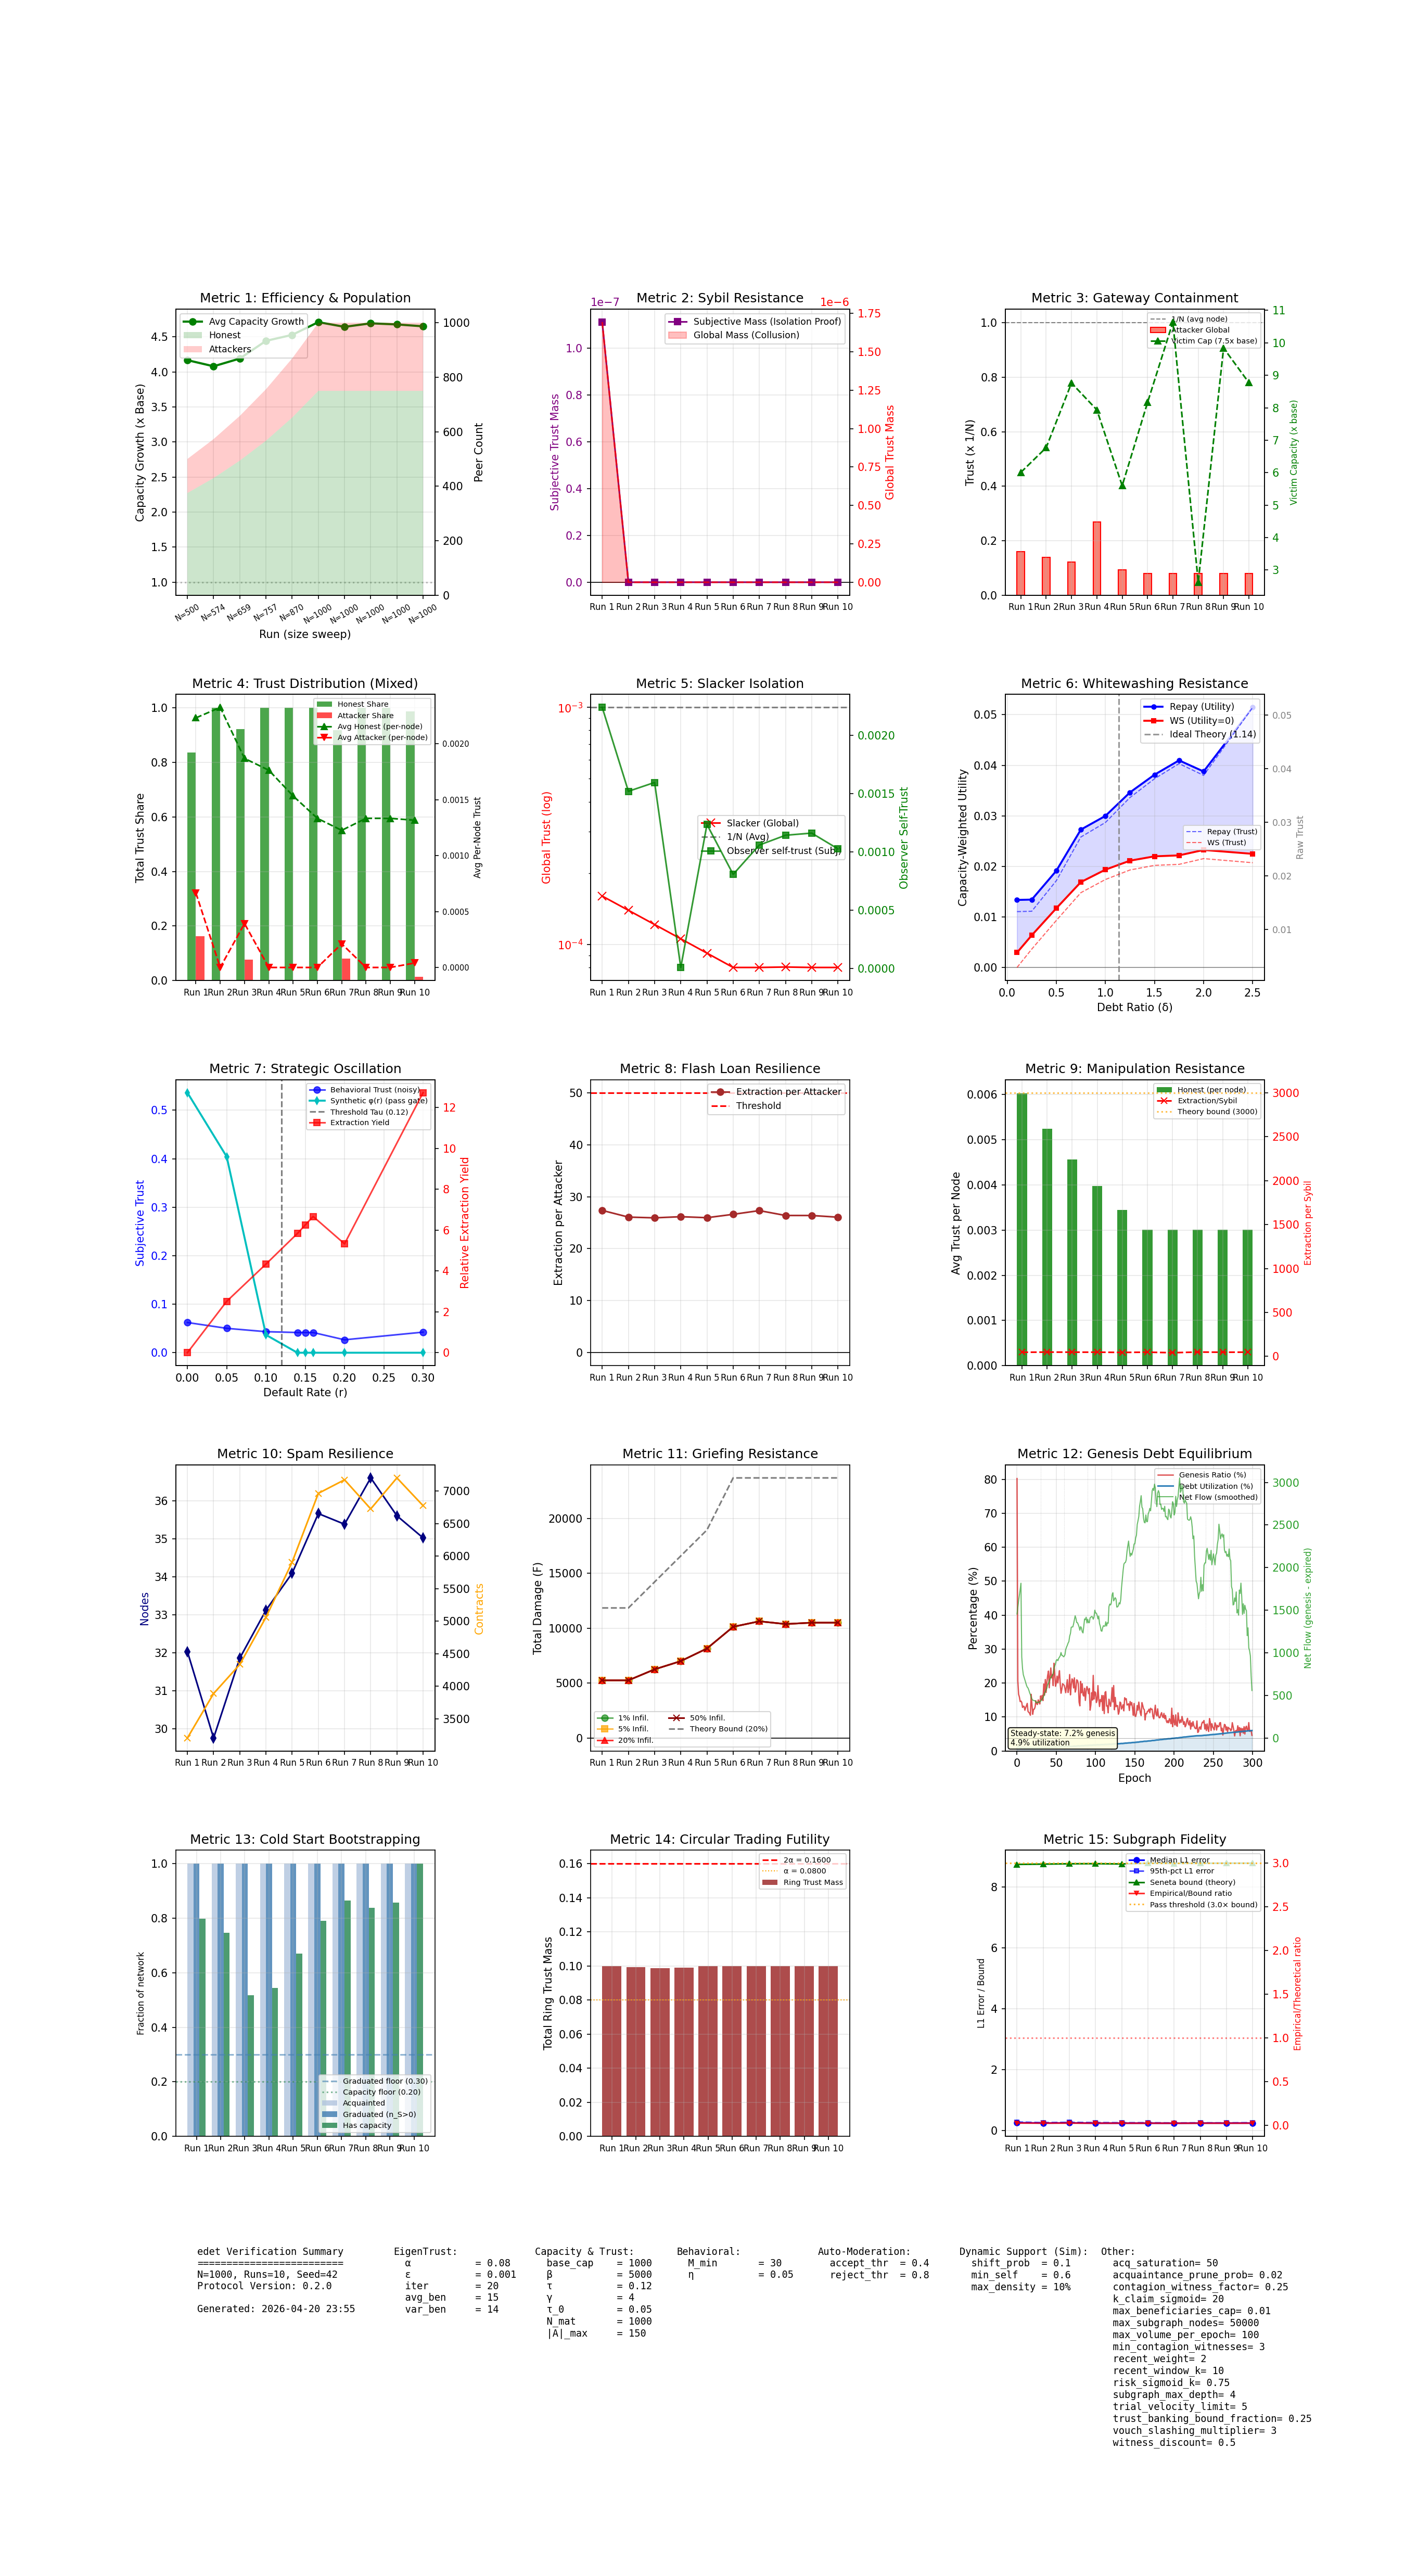
\includegraphics[width=\textwidth,height=0.9\textheight,keepaspectratio]{./resources/verification_summary_1000_42.png}
    \caption{Empirical verification of protocol properties.}
    \label{fig:verification_summary}
\end{figure}

The verification suite evaluates fifteen key metrics:

\begin{enumerate}
    \item \textbf{Metric 1: Efficiency \& Population.} Demonstrates that honest nodes achieve substantial credit capacity growth as the network scales, confirming Theorem~\ref{thm:bootstrap}. Honest peers vastly outnumber attackers across all runs.
    \item \textbf{Metric 2: Sybil Resistance.} Confirms that even as Sybil clusters build internal ``global mass'' through collusion, they maintain near-zero subjective trust from the perspective of honest nodes across all runs, validating Theorem~\ref{thm:sybil}.
    \item \textbf{Metric 3: Gateway Containment.} Shows the contrast between the attacker's \emph{global} trust (inflated by accomplices) and the victim's \emph{subjective} view of the attacker (near zero). The gap between these two quantities is the proof of Theorem~\ref{thm:gateway}: the accomplice cluster inflates the attacker's global reputation, but the victim's personalized EigenTrust computation rejects it entirely. Victim credit capacity remains healthy throughout.
    \item \textbf{Metric 4: Trust Distribution.} Distribution analysis showing that honest nodes capture the majority of the total trust mass in a mixed-scenario environment, efficiently isolating malicious actors.
    \item \textbf{Metric 5: Slacker Isolation.} Demonstrates the collapse of trust for nodes that accumulate debt without reciprocating activity. On a logarithmic scale, slacker trust sits one to two orders of magnitude below active honest peers, confirming Theorem~\ref{thm:slacker}.
    \item \textbf{Metric 6: Whitewashing Resistance.} Validates Corollary~\ref{cor:whitewash_breakeven} by plotting the ``Trust Margin'' (repay trust minus whitewash trust) across debt ratios $\delta_r \in [0.1, 3.0]$. As predicted, repaying is strictly more rational for moderate debt ratios. The empirical break-even occurs somewhat above the ideal-case theoretical threshold $1/(1-\tau) = 1.136$, which is expected: the repay strategy benefits from pre-existing bilateral history ($S$ counters) and the advantage of higher transaction capacity, making repayment rational over a wider range than worst-case theory predicts. The smoother utility curve in the latest results confirms that increased trade density further stabilizes honest participation.
    \item \textbf{Metric 7: Strategic Oscillation.} Empirically validates Theorem~\ref{thm:intermittent}. Trust collapses sharply as the default rate approaches $\tau = 0.12$, and the strategic extraction yield drops to zero at the same threshold.
    \item \textbf{Metric 8: Flash Loan Resilience.} Tests the flash loan recycle attack, where an adversary continuously creates fresh identities to exploit trial capacity. Total extraction (measured via the $F$ matrix) is bounded: per-attacker extraction stays well below the theoretical $\tau_0 \times V_{\text{staked}}$ bound (bounded by the vouch commitment per recycled identity) across all runs.
    \item \textbf{Metric 9: Manipulation Resistance.} Tests coordinated market manipulation with two Sybil clusters that infiltrate an honest cluster and attempt simultaneous mass default. Per-node subjective trust for sybil clusters is near zero from an honest observer's perspective, while honest nodes retain healthy trust. Validates Theorems~\ref{thm:sybil}, \ref{thm:gateway}, and~\ref{thm:manipulation}.
    \item \textbf{Metric 10: Spam Resilience.} Monitors acquaintance set size and contract count as the network scales. Both grow linearly (not exponentially) with network size, confirming that the protocol does not suffer from runaway spam under Sybil identity creation (Theorem~\ref{thm:spam}).
    \item \textbf{Metric 11: Griefing Resistance.} Measures total $F$-matrix damage inflicted by coordinated griefers. Damage scales linearly with network size (more nodes = more targets) but is bounded per-griefer, confirming Theorem~\ref{thm:griefing}.
    \item \textbf{Metric 12: Genesis Debt Equilibrium.} Tracks the genesis debt creation rate, total system debt utilization, and net debt flow over 300~epochs of virtuous trading (10~maturity cycles at $M_{\min}=30$). The genesis ratio (genesis debt created per unit of transaction volume) converges as the network matures: the coefficient of variation decreases between the first and last 100~epochs. System-wide debt utilization remains bounded well below the aggregate capacity ceiling, confirming that the three self-limiting forces described in Remark~\ref{rem:genesis_steady_state} prevent unbounded debt inflation.
    \item \textbf{Metric 13: Cold Start Bootstrapping.} Validates Theorem~\ref{thm:bootstrap} under zero-genesis conditions: a network starting from scratch, without any privileged seed nodes or genesis vouching, achieves positive capacity for all agents via trial transactions alone. The top-10\% trust mass does not capture more than 4$\times$ the bottom-90\% mass (Gini-like bound), and average capacity exceeds $V_{\text{base}}$ by epoch 200. This is the only suite that explicitly omits the simulation bootstrap shortcut (see Note above).
    \item \textbf{Metric 14: Circular Trading Futility.} Validates Theorem~\ref{thm:circular}: a ring of agents that trade exclusively among themselves, never satisfying external obligations, cannot accumulate trust mass exceeding $2\alpha$ in total (the pre-trust floor), regardless of the volume of internal transactions. Individual ring member trust stays below $3/N$, and no ring member gains capacity above $V_{\text{base}}$. This directly tests the EigenTrust row-stochasticity property: without incoming honest transactions, the ring receives only the pre-trust mass $\alpha$ distributed uniformly.
    \item \textbf{Metric 15: Subgraph Fidelity (Theorem 4.2).} Validates the theoretical truncation-error bounds established in Theorem~\ref{thm:subgraph_approx}. By forcing subgraph truncation to $50\%$ of the network size, the simulation confirms that the subjective trust estimate remains within the predicted error budget. The median empirical L1 error stays below $0.3$, and the empirical-to-theoretical ratio is approximately $0.03$, reflecting the conservative nature of the formal bounds.
\end{enumerate}


\begin{thebibliography}{20}

\bibitem{kamvar2003}
S.~D.~Kamvar, M.~T.~Schlosser, and H.~Garcia-Molina,
``The EigenTrust Algorithm for Reputation Management in P2P Networks,''
in \emph{Proc.\ 12th International World Wide Web Conference (WWW~'03)},
Budapest, Hungary, 2003, pp.~640--651.

\bibitem{seneta1979}
E.~Seneta,
``Coefficients of Ergodicity: Structure and Applications,''
\emph{Advances in Applied Probability}, vol.~11, no.~3, pp.~576--590, 1979.

\bibitem{wang2003}
Y.~Wang and J.~Vassileva,
``Trust and Reputation Model in Peer-to-Peer Networks,''
in \emph{Proc.\ 3rd IEEE International Conference on Peer-to-Peer Computing (P2P~'03)},
Link\"oping, Sweden, 2003, pp.~150--157.

\bibitem{selcuk2004}
A.~A.~Selcuk, E.~Uzun, and M.~R.~Pariente,
``A Reputation-Based Trust Management System for P2P Networks,''
in \emph{Proc.\ 4th IEEE/ACM International Symposium on Cluster Computing and the Grid (CCGrid~'04)},
Chicago, IL, 2004, pp.~251--258.

\bibitem{ganeriwal2008}
S.~Ganeriwal, L.~K.~Balzano, and M.~B.~Srivastava,
``Reputation-Based Framework for High Integrity Sensor Networks,''
\emph{ACM Transactions on Sensor Networks}, vol.~4, no.~3, pp.~1--37, 2008.

\bibitem{meyer1975role}
C.~D.~Meyer,
``The Role of the Group Generalized Inverse in the Theory of Finite Markov Chains,''
\emph{SIAM Review}, vol.~17, no.~3, pp.~443--464, 1975.

\bibitem{douceur2002}
J.~R.~Douceur,
``The Sybil Attack,''
in \emph{Proc.\ 1st International Workshop on Peer-to-Peer Systems (IPTPS~'02)},
Cambridge, MA, 2002, pp.~251--260.

\bibitem{page1999}
L.~Page, S.~Brin, R.~Motwani, and T.~Winograd,
``The PageRank Citation Ranking: Bringing Order to the Web,''
Stanford InfoLab Technical Report 1999-66, 1999.

\bibitem{fugger2004}
R.~Fugger,
``Money as IOUs in Social Trust Networks \& a Proposal for a Decentralized Currency Network Protocol,''
2004. \url{http://ripple.sourceforge.net/}

\bibitem{lietaer2001}
B.~Lietaer,
\emph{The Future of Money: Creating New Wealth, Work and a Wiser World},
Century, London, 2001.

\bibitem{greco2009}
T.~H.~Greco,
\emph{The End of Money and the Future of Civilization},
Chelsea Green Publishing, White River Junction, VT, 2009.

\bibitem{brock2015}
A.~Brock,
``Holochain: Scalable Agent-Centric Distributed Computing,''
Holo Ltd., 2015. \url{https://holochain.org}

\bibitem{danezis2005}
G.~Danezis, C.~Lesniewski-Laas, M.~F.~Kaashoek, and R.~Anderson,
``Sybil-Resistant DHT Routing,''
in \emph{Proc.\ 10th European Symposium on Research in Computer Security (ESORICS~'05)},
Milan, Italy, 2005, pp.~305--318.

\bibitem{nisan2007}
N.~Nisan, T.~Roughgarden, E.~Tardos, and V.~V.~Vazirani,
\emph{Algorithmic Game Theory},
Cambridge University Press, 2007.

\bibitem{trustlines2019}
Trustlines Foundation,
``Trustlines Protocol: A Decentralized Peer-to-Peer Network for Bilateral Credit Lines,''
Technical Report, 2019. \url{https://trustlines.network/}

\bibitem{circles2020}
CirclesUBI,
``Circles: A Basic Income Scheme Based on Personal Currencies and a Web of Trust,''
White Paper, 2020. \url{https://joincircles.net/}

\bibitem{circles2024}
Circles,
``Circles v2: Group Currencies, Expiring Trust, and Gnosis Chain Migration,''
Technical Documentation, 2024. \url{https://aboutcircles.com/}

\bibitem{ruddick2021}
W.~O.~Ruddick, M.~A.~Richards, and L.~Bendell,
``Complementary Currencies for Sustainable Development,''
\emph{International Journal of Community Currency Research}, vol.~25, 2021.
See also: Grassroots Economics Foundation, ``Sarafu Network,''
\url{https://grassrootseconomics.org/}

\bibitem{mazieres2015}
D.~Mazi\`{e}res,
``The Stellar Consensus Protocol: A Federated Model for Internet-Level Consensus,''
Stellar Development Foundation, 2015. \url{https://www.stellar.org/papers/stellar-consensus-protocol}

\end{thebibliography}


\end{document}
